\chapter{直线形}

在第一章里,我们从日常生活所熟悉的位置、通路、方
向、叠合出发,讨论了空间的几个重要的基本概念:点、直
线、平行、全等、相似,并通过观察、实验,分析归纳出了
空间的一些性质。在第二章中,我们把其中的某些性质作为
基本性质和定理。在本章中,我们将以这些基本性质和定理
为基础,运用第二章所介绍的演绎法去推演空间的其它性
质。演绎法不但是研究几何学的基本有效方法,在其它任何
科学的研究中也都是十分重要的方法。概括地说,对于科学
研究,实验归纳和论证推演是互相配合使用的两种基本科学
方法,它们是探索科学规律的两条腿。从这一章起,我们对
空间性质的探讨,主要用演绎法来进行。
\section{三角形}

\subsection{全等三角形}

\begin{blk}{定义}
    平面上顺次首尾端点相接且不在同一条直线上的
线段组成的封闭图形叫做\textbf{多边形}。这些线段叫做\textbf{多边形的边},
它们的端点叫做\textbf{多边形的顶点},每相邻两边的夹角叫做多边
形的\textbf{内角}。
\end{blk}


三角形是多边形中最简单的图形。有四条边的多边形叫
做四边形,有五条边的多边形叫五边形……等等。表示一个
多边形可用顶点的名称,沿周界顺次列出,如图3.1中的
$\triangle ABC$,四边形$ABCD$……等等。

如果多边形都在每边所在直线的同旁,我们称这种多边
形为\textbf{凸多边形}(图3.1中的三个图形都是凸多边形,图3.2
中的图形则不是)。以后我们说多边形时,都指的是凸多边
形。
\begin{figure}[htp]
    \centering
    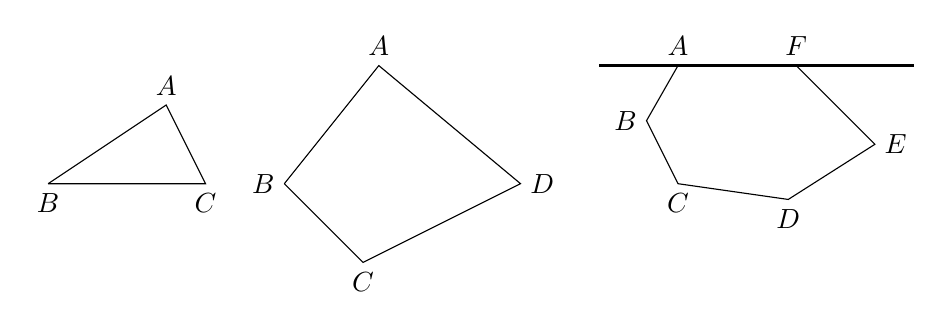
\begin{tikzpicture}
\begin{scope}
\draw(0,0)node[below]{$B$}--(2,0)node[below]{$C$}--(1.5,1)node[above]{$A$}--(0,0);
\end{scope}
\begin{scope}[xshift=3cm]
\draw (0,0)node[left]{$B$}--(1,-1)node[below]{$C$}--(3,0)node[right]{$D$}--(1.2,1.5)node[above]{$A$}--(0,0);
\end{scope}
\begin{scope}[xshift=8cm, yshift=1.5cm]
\draw (0,0)node[above]{$A$}--(1.5,0)node[above]{$F$}--(2.5,-1)node[right]{$E$}--(1.4,-1.7)node[below]{$D$}--(0,-1.5)node[below]{$C$}--(-.4,-.7)node[left]{$B$}--(0,0);
\draw[thick](-1,0)--(3,0);
\end{scope}        
    \end{tikzpicture}
    \caption{}
\end{figure}

\begin{figure}[htp]
    \centering
\begin{tikzpicture}
\draw[dashed](-2,0)--(2,0);
\draw (-.5,0)--(0.2,0)--(.3,-1)--(.7,1.8)--(-.5,0);
\end{tikzpicture}
    \caption{}
\end{figure}

\begin{blk}{定义}
两个能够完全叠合的三角形叫做\textbf{全等三角形}。两
个全等三角形完全叠合时,互相叠合的顶点叫做\textbf{对应点},互
相叠合的边叫做\textbf{对应边},互相叠合的角叫做\textbf{对应角}。因此,
\textbf{全等三角形的对应边相等,对应角相等}。
\end{blk}
 
怎样判定两个三角形全等呢?
\begin{enumerate}
\item 有两边和它们的夹角对应相等的两个三角形全
等。(SAS)
\item 有两角和它们的夹边对应相等的两个三角形全
等。(ASA)
\item 有三边对应相等的两个三角形全等。(SSS)
\end{enumerate}

利用三角形的全等,是判断两条线段或两个角相等的一
种基本方法。

\begin{example}
    在图3.3中,已知$\overline{AB}=\overline{AC}$, $\angle B=\angle C$
    
    求证:$\overline{BD}=\overline{CE}$.
\end{example}



\begin{analyze}
    要证$\overline{BD}=\overline{CE}$, 从图
上看$\overline{BD}$, $\overline{CE}$分别是$\triangle ABD$和
$\triangle ACE$的边,因此只要证明
$\triangle ACE \cong \triangle ABD$就行了,由已
知条件$\overline{AC}=\overline{AB}$, $\angle B=\angle C$而
$\angle A$是公共角,所以$\triangle ABD$与
$\triangle ACE$全等是很显然的。
\end{analyze}

\begin{proof}
在$\triangle ABD$与$\triangle ACE$中,

$\because\quad \overline{AB}=\overline{AC},\quad \angle B=\angle C$(已知)。

而$\angle A=\angle A$(公共角),

$\therefore\quad \triangle ABD\cong \triangle ACE$ (ASA).

$\therefore\quad \overline{BD}=\overline{CE}$ (全等三角形的对应边相等)。
\end{proof}    


\begin{figure}[htp]\centering
    \begin{minipage}[t]{0.48\textwidth}
    \centering
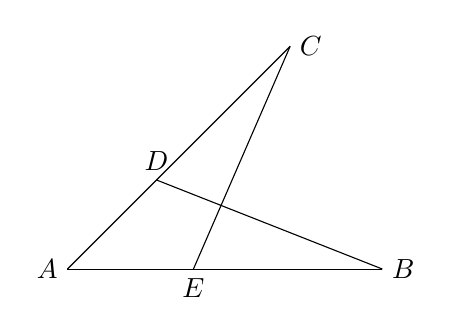
\begin{tikzpicture}[>=latex, scale=.8]
       \draw (0,0)node[left]{$A$}--(5,0)node[right]{$B$};
\draw (0,0)--(45:5)node[right]{$C$};
\draw (2,0)node[below]{$E$}--(45:5);
\draw (45:2)node[above]{$D$}--(5,0);
    \end{tikzpicture}
    \caption{}
    \end{minipage}
    \begin{minipage}[t]{0.48\textwidth}
    \centering
    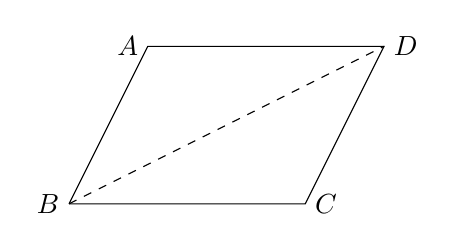
\begin{tikzpicture}[>=latex, scale=1]
        \draw (0,0)node[left]{$B$}--(3,0)node[right]{$C$}--(4,2)node[right]{$D$}--(1,2)node[left]{$A$}--(0,0);
        \draw[dashed](0,0)--(4,2);   
    \end{tikzpicture}
    \caption{}
    \end{minipage}
    \end{figure}


\begin{example}
    已知:在四边形$ABCD$中,$\overline{AD}=\overline{BC}$,
$\overline{AB}=\overline{CD}$(图3.4)。

求证:$\angle A=\angle C$。
\end{example}

\begin{analyze}
    要证明$\angle A=\angle C$, 
需要把四边形$ABCD$分成两个三
角形,为此,连结$B$、$D$. 这叫
做添\textbf{辅助线}。这样只需证
$\triangle ABD\cong \triangle CDB$就行了。
\end{analyze}

\begin{proof}
连结$B$、$D$, 在$\triangle ABD$与$\triangle CDB$中,

$\because\quad \overline{AD}=\overline{BC},\quad \overline{AB}=\overline{CD}$ (已知)

又$\because\quad \overline{BD}=\overline{BD}$ (公共边)

$\therefore\quad \triangle ABD\cong \triangle CDB$ (SSS)

$\therefore\quad \angle A=\angle C$(全等三角形的对应角相等)。
\end{proof}    

\begin{example}
在图3.5中,已知:$\overline{AB}=\overline{CD}$, $\angle B=\angle CDF$, $\overline{BD}=\overline{EF}$.

求证:$\overline{AE}=\overline{CF}$.
\end{example}

\begin{analyze}
    要证$\overline{AE}=\overline{CF}$, 只需证$\triangle ABE\cong \triangle CDF$. 由已
知,$\overline{AB}=\overline{CD}$, $\angle B=\angle CDF$, $\overline{BD}=\overline{EF}$, 虽然不能马上说
$\triangle ABE$和$\triangle CDF$全等,但只要注意到$\overline{BD}+\overline{DE}=\overline{DE}+\overline{EF}$, 
即$\overline{EB}=\overline{DF}$就行了。
\end{analyze}

\begin{proof}
    在图3-5中,$\because\quad \overline{BD}=\overline{EF}$ 已知

$\therefore\quad \overline{BD}+\overline{DE}=\overline{DE}+\overline{EF}$ (等量加等量和相等)。即:
\[\overline{BE}=\overline{DF}\]
又$\because\quad \overline{AB}=\overline{CD},\; \angle B =\angle CDF$ 已知

$\therefore\quad \triangle ABE\cong \triangle CDF$ (SAS).

$\therefore\quad \overline{AE}=\overline{CF}$ (全等三角形的对应边相等)。
\end{proof}

\begin{figure}[htp]\centering
    \begin{minipage}[t]{0.48\textwidth}
    \centering
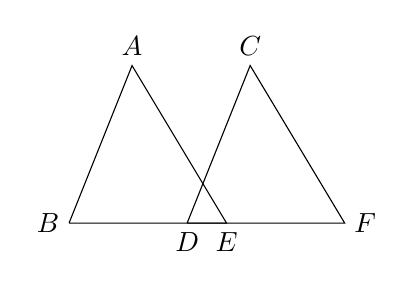
\begin{tikzpicture}[>=latex, scale=1]
       \draw(0,0)node[left]{$B$}--(2,0)node[below]{$E$}--(.8,2)node[above]{$A$}--(0,0);
\draw(1.5,0)node[below]{$D$}--(3.5,0)node[right]{$F$}--(2.3,2)node[above]{$C$}--(1.5,0);
    \end{tikzpicture}
    \caption{ }
    \end{minipage}
    \begin{minipage}[t]{0.48\textwidth}
    \centering
    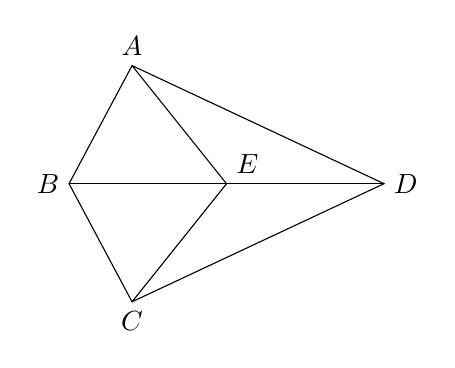
\begin{tikzpicture}[>=latex, xscale=.8]
      \draw(0,0)node[left]{$B$}--(5,0)node[right]{$D$};
      \draw(1,1.5)node[above]{$A$}--(2.5,0)node[above right]{$E$}--(1,-1.5)node[below]{$C$}--(0,0)--(1,1.5)--(5,0)--(1,-1.5);
    \end{tikzpicture}
    \caption{ }
    \end{minipage}
    \end{figure}

\begin{example}
    在图3.6中,已知:$\overline{AB}=\overline{BC}$, $\overline{AD}=\overline{CD}$, $E$点在$BD$上。

求证:$\overline{AE}=\overline{CE}$.
\end{example}

\begin{analyze}
    要证$\overline{AE}=\overline{CE}$, 只需证明$\triangle ABE\cong \triangle CBE$, 或者证明$\triangle ADE\cong \triangle CDE$, 假定我们证明$\triangle ABE\cong \triangle CBE$,
    已知$\overline{AB}=\overline{BC}$, $\overline{BE}=\overline{BE}$, 因此只需证明$\angle ABD=\angle CBD$;
    要证$\angle ABD=\angle CBD$, 只需证明$\triangle ABD\cong\triangle CBD$.
\end{analyze}

\begin{proof}
    在$\triangle ABD$与$\triangle CBD$中,

    $\because\quad \overline{AB}=\overline{CB},\quad \overline{AD}=\overline{CD}$ (已知)   $\overline{BD}=\overline{BD}$(公共边)

    $\therefore\quad \triangle ABD\cong \triangle CBD$ (SSS).

    $\therefore\quad \angle ABD=\angle CBD$ (全等三角形的对应角相等)

$\because\quad     \overline{AB}=\overline{BC}$ (已知) 
    $\overline{BE}=\overline{BE}$ (公共边)

$\therefore\quad \triangle ABE\cong \triangle CBE$ (SAS).

$\therefore\quad \overline{AE}=\overline{CE}$ (全等三角形的对应边相等)。
\end{proof}

    利用三角形全等,来证明两条线段或两个角相等,关键
    在于找出能够全等的三角形,并且使要证明的线段和角恰好
    成为它们的对应边和对应角。为了找出全等的三角形,必要
    时需要添加辅助线。  

\begin{ex}
\begin{enumerate}
    \item 已知:在四边形$ABCD$中,$AC$平分$\angle BAD$, $\overline{AB}=\overline{AD}$.
    
    求证:$\angle ACB=\angle ACD$.
    \item 已知:如图,$\overline{AC}$、$\overline{BD}$交于$O$点,    且$\overline{AO}=\overline{OC}$、$\overline{BO}=\overline{OD}$.
    
    求证:$\overline{AB}=\overline{CD}$.


\item 已知:如图,$\angle 1=\angle 4$, $\angle 2=\angle 3$.
求证:$\overline{AB}=\overline{CD}$.
\item 已知:如图,$\angle 1=\angle 2$, $\angle 3=\angle 4$, $\overline{AB}=\overline{AD}$. 

求证:$\overline{AE}=\overline{AC}$, $\angle E=\angle C$.

\item 已知:如图,$\angle 1=\angle 2$, $\angle 3=\angle 4$,
求证:$\overline{AC}=\overline{BD}$.
\item 已知:如图,在四边形$ABCD$中,$\overline{AB}=\overline{BC}$, $\overline{AD}=\overline{CD}$.

求证:$\angle A=\angle C$.
\item 已知:如图,$\overline{AD}=\overline{BE}$, $\overline{AE}=\overline{BD}$, AC、BC是直线。

求证:$\angle CDB=\angle CEA$.
\item 已知:如图,$\overline{AB}=\overline{CD}$, E、F分别是$\overline{AB}$、$\overline{CD}$的中点,
并且$\overline{BF}=\overline{CE}$.

求证:$\angle EBC=\angle FCB$, $\angle FBC=\angle ECB$.

\item 已知:如图,在四边形$ABCD$中,$\overline{AB}=\overline{CD}$, $\overline{AD}=\overline{BC}$, $\overline{EF}$过$\overline{BD}$的中点$O$. 

求证:$\overline{OE}=\overline{OF}$.
\end{enumerate}
\end{ex}

\begin{figure}[htp]\centering
    \begin{minipage}[t]{0.48\textwidth}
    \centering
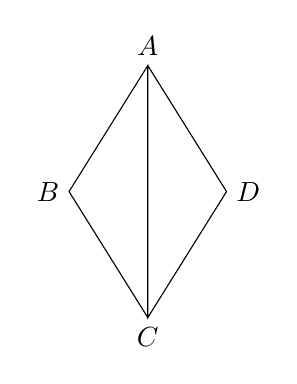
\begin{tikzpicture}[>=latex, yscale=.8]
       \draw(0,2)node[above]{$A$}--(1,0)node[right]{$D$}--(0,-2)node[below]{$C$}--(0,2)--(-1,0)node[left]{$B$}--(0,-2);
    \end{tikzpicture}
    \caption*{第1题}
    \end{minipage}
    \begin{minipage}[t]{0.48\textwidth}
    \centering
    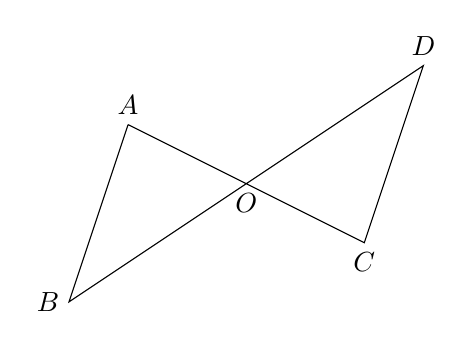
\begin{tikzpicture}[>=latex, scale=1.5]
      \draw(-1,.5)node[above]{$A$}--(1,-.5)node[below]{$C$}--(1.5,1)node[above]{$D$}--(-1.5,-1)node[left]{$B$}--(-1,.5);
      \node at (0,0)[below]{$O$};
    \end{tikzpicture}
    \caption*{第2题}
    \end{minipage}
    \end{figure}

\begin{figure}[htp]\centering
    \begin{minipage}[t]{0.48\textwidth}
    \centering
\begin{tikzpicture}[>=latex, scale=1.3]
\tkzDefPoints{1/2/A, 0/0/B, 3/0/C, 4/2/D}
\tkzDrawPolygon(A,B,C)
\tkzDrawPolygon(A,D,C)
\tkzMarkAngle[mark=none, size=.35](B,A,C)  
\tkzLabelAngle[pos=.5](B,A,C) {2}
\tkzMarkAngle[mark=none, size=.5](C,A,D)  
\tkzLabelAngle[pos=.7](C,A,D) {1}
 \tkzLabelAngle[pos=.75](A,C,B) {4}
\tkzMarkAngle[mark=none, size=.5](D,C,A)  
\tkzLabelAngle[pos=.25](D,C,A) {3}
\tkzMarkAngle[mark=none, size=.6](A,C,B) 
\tkzLabelPoints[left](A,B)
\tkzLabelPoints[right](C,D)
    \end{tikzpicture}
    \caption*{第3题}
    \end{minipage}
    \begin{minipage}[t]{0.48\textwidth}
    \centering
    \begin{tikzpicture}[>=latex, scale=1.3]
        \tkzDefPoint(0,0){A}
        \tkzDefPoint(-90:2){B}
        \tkzDefPoint(-60:2){D}
        \tkzDefPoint(0:2.75){E}
        \tkzDefPoint(-30:2.75){C}
        \tkzLabelPoints[left](A,B)
        \tkzDrawPolygon(A,B,D)
\tkzDrawLines[add=0 and 1.38](B,D) %\tkzGetPoint{C}
\draw (D)--(E)--(A)--(C);
\tkzLabelPoints[right](C,E)
\tkzLabelPoints[below](D)
\tkzMarkAngles[mark=none, size=.44](C,A,E B,A,D C,B,A E,D,A)  
\tkzLabelAngle[pos=.65](C,A,E) {2}
\tkzLabelAngle[pos=.65](B,A,D) {1}
\tkzLabelAngle[pos=.6](C,B,A) {3}
\tkzLabelAngle[pos=.6](E,D,A) {4}


    \end{tikzpicture}
    \caption*{第4题}
    \end{minipage}
    \end{figure}



\begin{figure}[htp]\centering
    \begin{minipage}[t]{0.48\textwidth}
    \centering
\begin{tikzpicture}[>=latex, scale=1]
\tkzDefPoints{-1/2/A, 1/2/D, -2/-1/B, 2/-1/C}
\tkzDrawPolygon(A,C,D) \tkzDrawPolygon(A,B,D)
\tkzLabelPoints[left](A,B)
\tkzLabelPoints[right](C,D)
\tkzMarkAngles[mark=none, size=.6](C,A,D A,D,B) 
\tkzMarkAngles[mark=none, size=.5](B,A,C B,D,C) 
\tkzLabelAngle[pos=.7](C,A,D) {1}
\tkzLabelAngle[pos=.7](A,D,B) {2}
\tkzLabelAngle[pos=.65](B,A,C) {3}
\tkzLabelAngle[pos=.65](B,D,C) {4}



    \end{tikzpicture}
    \caption*{第5题}
    \end{minipage}
    \begin{minipage}[t]{0.48\textwidth}
    \centering
    \begin{tikzpicture}[>=latex, scale=1.3]
        \tkzDefPoints{-1/0/B, 2/0/D, 1/1/A, 1/-1/C, 0/0/O} 
        \tkzDrawPolygon(A,B,C,D)
        \tkzAutoLabelPoints[center=O](A,B,C,D)

    \end{tikzpicture}
    \caption*{第6题}
    \end{minipage}
    \end{figure}




\begin{figure}[htp]\centering
    \begin{minipage}[t]{0.48\textwidth}
    \centering
\begin{tikzpicture}[>=latex, scale=1]
    \tkzDefPoints{-1.5/0/A, 1.5/0/B, 0/3/C, 0/1.5/O}  
    \tkzDefMidPoint(A,C)\tkzGetPoint{D}
    \tkzDefMidPoint(B,C)\tkzGetPoint{E}    
    \tkzDrawPolygon(A,B,C)
    \draw(B)--(D)node[left]{$D$};
    \draw (A)--(E)node[right]{$E$};
    \tkzAutoLabelPoints[center=O](A,B,C)
    \end{tikzpicture}
    \caption*{第7题}
    \end{minipage}
    \begin{minipage}[t]{0.48\textwidth}
    \centering
    \begin{tikzpicture}[>=latex, scale=.8]
        \tkzDefPoints{-2.5/0/B, 2.5/0/C, -1.5/3/A, 1.5/3/D,  0/1.5/O}  
        \tkzDefMidPoint(A,B)\tkzGetPoint{E}
        \tkzDefMidPoint(D,C)\tkzGetPoint{F}    
        \tkzDrawPolygon(A,B,C,D)
        \draw(B)--(F)node[right]{$F$};
        \draw (C)--(E)node[left]{$E$};
        \tkzAutoLabelPoints[center=O](A,B,C,D)
    \end{tikzpicture}
    \caption*{第8题}
    \end{minipage}
    \end{figure}


\begin{figure}[htp]\centering
    \begin{minipage}[t]{0.48\textwidth}
    \centering
\begin{tikzpicture}[>=latex, scale=.8]
    \tkzDefPoints{-2.5/0/B, 2.5/0/C, -1.5/3/A, 3.5/3/D}  
    \tkzDefMidPoint(D,B)\tkzGetPoint{O}
    \tkzDrawPolygon(A,B,C,D)
\draw (0,3)node[above]{$E$}--(1,0)node[below]{$F$};
\tkzAutoLabelPoints[center=O](A,B,C,D)
\draw(B)--(D);
\node at (O)[right]{$O$};

    \end{tikzpicture}
    \caption*{第9题}
    \end{minipage}
    \begin{minipage}[t]{0.48\textwidth}
    \centering
    \begin{tikzpicture}[>=latex, scale=1]
\tkzDefPoints{-1.5/0/B, 1.5/0/C, 0/3/A, 0/1.5/O}
\tkzDrawPolygon(A,B,C)
\tkzAutoLabelPoints[center=O](A,B,C)
\tkzMarkAngles[mark=none, size=.5](C,B,A A,C,B B,A,C) 
\node at (0,-.25){底};\node at (0,2.25){顶角};
\node at (-1,1.5){腰};\node at (1,1.5){腰};
\node(A) at (0,.25){底角};
\draw[<-](-1,.25)--(A);
\draw[<-](1,.25)--(A);
    \end{tikzpicture}
    \caption{}
    \end{minipage}
    \end{figure}

\subsection{等腰三角形}

\begin{blk}{定义}
    有两条边相等的三角形叫做\textbf{等腰三角形}。相等的两边
叫做\textbf{腰},另外的一边叫做\textbf{底},腰和底的夹角叫做\textbf{底角},两腰的夹
角叫\textbf{顶角},如图3.7所示。
\end{blk}

\begin{blk}{定义}
    三角形的一个角的平分线与对边相交,这个角的
    顶点和交点之间的线段叫做\textbf{三角形的角的平分线}。在图
    3.8(1)中,$\overline{AF}$平分$\angle A$, 交对边于$F$点,$\overline{AF}$就是$\triangle ABC$
    的$\angle A$的平分线。  

    连结三角形一个顶点和它的对边中点的线段叫做\textbf{三角形
的中线}。在图3.8(2)中,$E$点是$\overline{BC}$的中点,$\overline{AF}$就是$\triangle ABC$的$\overline{BC}$边上的中线。

从三角形一个顶点到它的对边所在直线作垂线,顶点和
垂足之间的线段叫做\textbf{三角形的高线}(简称\textbf{高})。在图3.8(3)
中,$\overline{AD}\bot$直线$BC$, $D$是垂足,$\overline{AD}$就是$\triangle ABC$的$\overline{BC}$边上
的高线。
\end{blk}

\begin{figure}[htp]
    \centering
\begin{tikzpicture}[scale=.8]
\begin{scope}
\tkzDefPoints{0/0/B, 3.6/0/F, 5.5/0/C, 4.5/3/A}
\tkzDrawPolygon(A,B,C)
\draw(A)--(F);
\tkzMarkAngles[mark=none, size=.5](B,A,F) 
\tkzMarkAngles[mark=none, size=.6](F,A,C)
\tkzLabelAngle[pos=.7](B,A,F) {1}
\tkzLabelAngle[pos=.75](F,A,C) {2}

\tkzLabelPoints[below](C, F, B)
\tkzLabelPoint(A){$A$}
\node at (2.7,-1){(1)};
\end{scope}
\begin{scope}[xshift=7cm]
    \tkzDefPoints{0/0/B, 2/0/E, 4/0/C, 4.5/3/A}
    \tkzDrawPolygon(A,B,C)
    \tkzLabelPoints[below](C, E, B)
    \tkzLabelPoint(A){$A$}
    \draw(E)--(A);
    \node at (2.2,-1){(2)};
\end{scope}    
\begin{scope}[yshift=-5cm]
\draw (0,0)node[below]{$B$}--(5.5,0)node[below]{$C$}--(4.5,3)node[above]{$A$}--(0,0);
\tkzDefPoints{4.5/3/A1, 4.5/0/D1, 5.5/0/C1}
\tkzMarkRightAngle(A1,D1,C1)
\draw(4.5,3)--(4.5,0)node[below]{$D$};
\draw(11,3)--(11,0)node[below]{$D$};
\draw[dashed](9,0)--(12,0);
\draw (7,0)node[below]{$B$}--(9.5,0)node[below]{$C$}--(11,3)node[above]{$A$}--(7,0);
\tkzDefPoints{11/3/A2, 11/0/D2, 9.5/0/C2}
\tkzMarkRightAngle(A2,D2,C2)
\node at (6,-1){(3)};
\end{scope}
\end{tikzpicture}
    \caption{}
\end{figure}

三角形的高线、中线、角平分线,一般是指一条线段,
但有时当我们不考虑其长度时,也把它们分别所在的直线叫
做三角形的高线、中线、角的平分线。


\begin{blk}
    {等腰三角形性质定理} 等腰三角形底角相等。
\end{blk}

已知:在$\triangle ABC$中;$AB=AC$.
求证:$\angle B=\angle C$.

\begin{figure}[htp]
    \centering
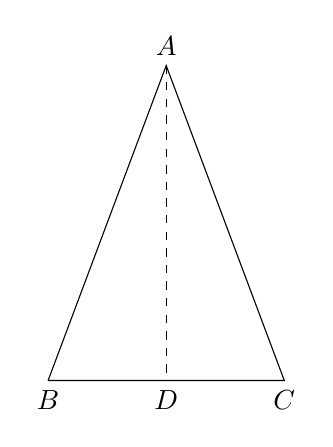
\begin{tikzpicture}
\draw (0,0)node[below]{$B$}--(3,0)node[below]{$C$}--(1.5,4)node[above]{$A$}--(0,0);
\draw[dashed](1.5,4)--(1.5,0)node[below]{$D$};
\end{tikzpicture}
    \caption{}
\end{figure}
\begin{proof}
    作$\angle BAC$的平分线$\overline{AD}$
(图3.9),在$\triangle ABD$和$\triangle ACD$
中

$\because\quad AB=AC$ (已知),$\overline{AD}=\overline{AD}$(公共边),$\angle BAD=\angle CAD$(角平分线定义)

$\therefore\quad \triangle ABD≤\triangle ACD$(SAS)

$\therefore\quad \angle B=\angle C$(全等三角形的对应角相等)。
\end{proof}


由于 $\overline{BD}=\overline{DC},\; \angle BDA=\angle CDA=90^{\circ}$

因此 $AD$平分$\overline{BC}$, 且$AD\bot BC$.

\begin{blk}{推论 }
    等腰三角形顶角的平分线垂直、平分底边。
\end{blk}

也就是说,等腰三角形的顶角平分线也是底边上的高线
和中线。(\textbf{三线合一})

\begin{blk}
    {等腰三角形的判定定理} 有两个角相等的三角形是等腰
三角形。
\end{blk}

已知:在$\triangle ABC$中,$\angle B=\angle C$(图3.10)。
求证:$\overline{AB}=\overline{AC}$.

\begin{figure}[htp]
    \centering
\begin{tikzpicture}
\draw(0,0)node[left]{$B$}--(2,0)node[right]{$C$}--(1,2)node[above]{$A$}--(0,0);
\draw(4,2)node[left]{$B'$}--(6,2)node[right]{$C'$}--(5,0)node[below]{$A'$}--(4,2);
\end{tikzpicture}
    \caption{}
\end{figure}


\begin{proof}
    根据翻转公理,我们可以把$\triangle ABC$翻转过来,
    设顶点$A$、$B$、$C$成为$A'$、$B'$、$C'$.
    
    $\because\quad \angle B=\angle C=\angle C',\quad \angle C=\angle B=\angle B'$

    又:$\because\quad \overline{BC}=\overline{C'B'}$

    $\therefore\quad \triangle ABC\cong \triangle A'C'B'$(ASA)

    $\therefore\quad \overline{AB}=\overline{A'C'}$(全等三角形的对应边相等)。

由于$\overline{AC}=\overline{A'C'}$,$\therefore\quad \overline{AB}=\overline{AC}$(等量代换)
\end{proof}

用逻辑语句说:等腰三角形的判定定理是其性质定理的
逆定理。这两个定理我们用“充要”条件可合写成一个定理:

\begin{blk}{}
   一个三角形是等腰三角形的充要条件是这个三角形有两
个角相等。
\end{blk}


\begin{blk}{定义}
    三条边都相等的三角形叫做\textbf{等边三角形},也叫做
    \textbf{正三角形}。
\end{blk}


同学们自己证明下面等边三角形的性质定理和判定定
理。

\begin{blk}{}
    \begin{itemize}
        \item 等边三角形的三内角相等。
        \item   三内角相等的三角形是等边三角形。
    \end{itemize}
\end{blk}

由等腰三角形及等边三角形的性质定理和判定定理可
知,在一个三角形中,由边的相等可以推知角的相等,反过
来由角的相等也可推知边的相等。下面举例说明它们在证题
中的应用。

\begin{example}
已知:在图3.11中,$\overline{AB}=\overline{EB}$, 
$\overline{AC}=\overline{DC}$, 
ADB、AEC是直线。

求证:$\angle ADC=\angle AEB$.
\end{example}

\begin{analyze}
    要证$\angle ADC=\angle AEB$,
只需证明$\angle ADC=\angle A$, $\angle AEB=\angle A$; 要证明
$\angle ADC=\angle A$, $\angle AEB=\angle A$, 只要知道$\overline{AC}=\overline{DC}$, 
$\overline{AB}=\overline{BE}$就行了。
\end{analyze}

\begin{proof}
    在$\triangle BAE$中,
$\because\quad \overline{AB}=\overline{EB}$(已知),

$\therefore\quad \angle AEB=\angle A$(等腰三角形的底角相等)。

在$\triangle CAD$中,
$\because\quad \overline{AD}=\overline{DC}$(已知),

$\therefore\quad \angle ADC=\angle A$(等腰三角形的底角相等)。

$\therefore\quad \angle ADC=\angle AEB$ (等量代换)。
\end{proof}

\begin{figure}[htp]\centering
    \begin{minipage}[t]{0.48\textwidth}
    \centering
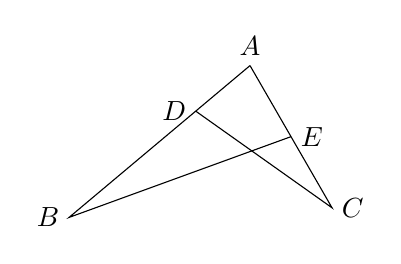
\begin{tikzpicture}[>=latex, scale=1]
\draw(40:3)node[above]{$A$}--(0,0)node[left]{$B$}--(20:3)node[right]{$E$};
\draw(40:3)--(3.34,0.122)node[right]{$C$}--(40:2.1)node[left]{$D$};
    \end{tikzpicture}
    \caption{}
    \end{minipage}
    \begin{minipage}[t]{0.48\textwidth}
    \centering
    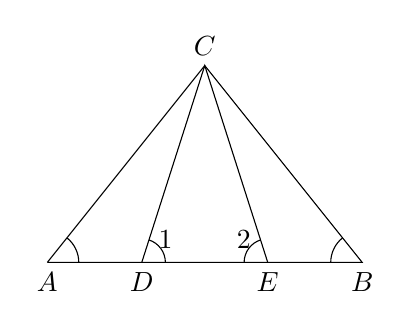
\begin{tikzpicture}[>=latex, scale=1]
\draw(-2,0)node[below]{$A$}--(0,2.5)node[above]{$C$}--(2,0)node[below]{$B$}--(-2,0);
\draw(.8,0)node[below]{$E$}--(0,2.5)--(-.8,0)node[below]{$D$};
\draw (-2+.4,0) arc (0:51.34:.4);
\draw (2-.4,0) arc (180:180-51.34:.4);
\draw (-.8+.3,0) arc (0:72.3:.3)node[right]{1};
\draw (.8-.3,0) arc (180:180-72.3:.3)node[left]{2};
    \end{tikzpicture}
    \caption{}
    \end{minipage}
    \end{figure}


\begin{example}
    如图3.12, 
己知:$\overline{AC}=\overline{BC}$, $\overline{AE}=\overline{DB}$. 

求证:$\overline{CD}=\overline{CE}$.
\end{example}

\begin{analyze}
    在$\triangle CDE$中,若要证$\overline{CD}=\overline{CE}$,
   只要证$\angle 1=\angle 2$即可, $\angle 1$和$\angle 2$分别在$\triangle BCD$与$\triangle ACE$中,如能证明$\triangle BCD\cong \triangle ACE$, 即可证明$\angle 1=\angle 2$.
\end{analyze}

\begin{solution}
在$\triangle ACE$与$\triangle BCD$中,

$\because\quad \overline{AC}=\overline{BC},\quad \overline{AE}=\overline{BD}$ (已知)

$\therefore\quad \angle A=\angle B$(等腰三角形两底角相等),

$\therefore\quad \triangle ACE\cong \triangle BCD$(SAS)

$\therefore\quad \angle 2=\angle 1$(全等三角形的对应角相等),

$\therefore\quad \triangle CDE$ 是等腰三角形(有两角相等的三角形是等腰三角形)。

$\therefore\quad \overline{CD}=\overline{CE}$
\end{solution}

\begin{ex}
\begin{enumerate}
    \item 画出$\triangle ABC$和$\triangle DEF$的三条边上的高线。
    \item 画一个三角形$ABC$, 然后画出$\triangle ABC$三个内角的平分线。
    \item 画一个三角形$DEF$, 然后画出$\triangle DEF$三边上的中线。
    \item 证明:全等三角形的对应角的平分线相等。
    \item 证明:全等三角形对应边上的中线相等。
    \item 已知:$A=\{\text{等腰三角形}\}$,$B=\{\text{两内角相等的三角
    形}\}$,指出集合$A$与集合$B$的关系。
    \item 若$\overline{AC}=\overline{BC},\quad \angle DCA=\angle ECB$, 则$\overline{CD}=\overline{CE}$.
    \item 若$\overline{AC}=\overline{BC},\quad \angle 1=\angle 2$, 则$\overline{AE}=\overline{BD}$.
    \item 若$\overline{AC}=\overline{BC}$, $\overline{AD}$、$\overline{BE}$分别是$\angle A$和$\angle B$的平分线,
    则$\overline{AD}=\overline{BE}$.
    \item 若$\overline{AC}=\overline{BC},\quad \overline{AD}=\overline{BE}$, $DE$是直线,则$\triangle DEC$是等腰
三角形。
\item 若$\overline{AC}=\overline{BC},\quad \angle ACD=\angle BCE$, $DE$是直线,则$\triangle DEC$
是等腰三角形。
\item 在等边$\triangle ABC$的三边上,分别取$D$、$E$、$F$(如图),
使$\overline{AD}=\overline{BE}=\overline{CF}$, 则$\triangle DEF$是等边三角形。
\item 设$\overline{DE}=\overline{EF}=\overline{FD}$, $\angle AFD=\angle BDE=\angle CEF$, 
则$\triangle ABC$是等边三角形。
\end{enumerate}
\end{ex}

\begin{figure}[htp]
    \centering
\begin{tikzpicture}
\begin{scope}
    \draw(0,0)node[below]{$B$}--(1.5,.2)node[below]{$C$}--(2,2)node[above]{$A$}--(0,0);
\end{scope}
\begin{scope}[xshift=5cm]
    \draw(0,0)node[below]{$E$}--(2,0)node[below]{$F$}--(.7,1.5)node[above]{$D$}--(0,0);
\end{scope}
\end{tikzpicture}
    \caption*{第1题}
\end{figure}

\begin{figure}[htp]\centering
    \begin{minipage}[t]{0.48\textwidth}
    \centering
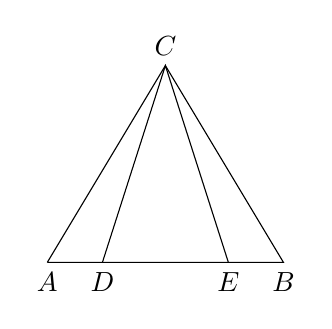
\begin{tikzpicture}[>=latex, scale=1]
\draw(-1.5,0)node[below]{$A$}--(0,2.5)node[above]{$C$}--(1.5,0)node[below]{$B$}--(-1.5,0);
\draw(.8,0)node[below]{$E$}--(0,2.5)--(-.8,0)node[below]{$D$};
    \end{tikzpicture}
    \caption*{第7题}
    \end{minipage}
    \begin{minipage}[t]{0.48\textwidth}
    \centering
    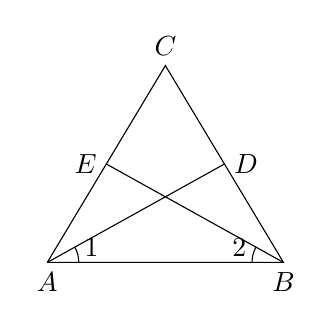
\begin{tikzpicture}[>=latex, scale=1]
\draw(-1.5,0)node[below]{$A$}--(0,2.5)node[above]{$C$}--(1.5,0)node[below]{$B$}--(-1.5,0);
\draw(-.75,1.25)node[left]{$E$}--(1.5,0);
\draw(.75,1.25)node[right]{$D$}--(-1.5,0);
\draw(-1.5+.4,0) arc (0:29:.4)node[right]{1};
\draw(1.5-.4,0) arc (180:180-29:.4)node[left]{2};
    \end{tikzpicture}
    \caption*{第8--9题}
    \end{minipage}
    \end{figure}

\begin{figure}[htp]\centering
    \begin{minipage}[t]{0.48\textwidth}
    \centering
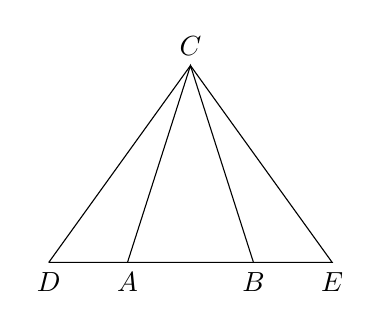
\begin{tikzpicture}[>=latex, scale=1]
    \draw(-1.8,0)node[below]{$D$}--(0,2.5)node[above]{$C$}--(1.8,0)node[below]{$E$}--(-1.8,0);
    \draw(.8,0)node[below]{$B$}--(0,2.5)--(-.8,0)node[below]{$A$};
    \end{tikzpicture}
    \caption*{第10--11题}
    \end{minipage}
    \begin{minipage}[t]{0.48\textwidth}
    \centering
    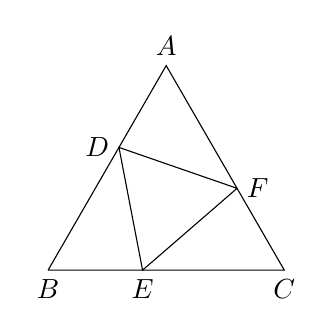
\begin{tikzpicture}[>=latex, scale=1]
\draw(-120:3)node[below]{$B$} --(0,0)node[above]{$A$}--(-60:3)node[below]{$C$}-- (-120:3) ;
\draw(-60:1.8)node[right]{$F$}--(-120:1.2)node[left]{$D$}--(-.3,-1.5*1.732)node[below]{$E$}--(-60:1.8);
    \end{tikzpicture}
    \caption*{第12--13题}
    \end{minipage}
    \end{figure}

\subsection{轴对称图形}
\begin{blk}{定义}
    在平面上有两个图形$F$和$F'$, 如果平面沿着某
条直线$\ell$折叠起来,$F$和$F'$叠合,就称$F$和$F'$关于$\ell$成\textbf{轴对
称}。(也称$F$和$F'$是以$\ell$为轴的\textbf{对称形})。$F$和$F'$上互相叠合
的点叫做\textbf{对称点},$\ell$叫做\textbf{对称轴}。
\end{blk}

在图3.13(1)中,平面上的$\triangle ABC$和$\triangle A'B'C'$关于直
线$\ell$成轴对称;$A$与$A'$、$B$与$B'$、$C$与$C'$都是对称点。

\begin{figure}[htp]
    \centering
\begin{tikzpicture}
\begin{scope}
    \draw(0,-.5)--(0,4)node[above]{$\ell$};
    \node at (0,-1){(1)};

\draw(-1.8,2)node[above]{$B$}--(-.4,3)node[above]{$A$}--(-1.4,0.5)node[below]{$C$}--(-1.8,2);
\draw(1.8,2)node[above]{$B'$}--(.4,3)node[above]{$A'$}--(1.4,0.5)node[below]{$C'$}--(1.8,2);

\end{scope}
\begin{scope}[xshift=6.5cm]
    \draw(0,-.5)--(0,4)node[above]{$\ell$};
\draw(-2,0)node[below]{$B$}--(2,0)node[below]{$C$}--(0,3)node[right]{$A$}--(-2,0);
\draw (0,0) rectangle (.2,.2);
\node at (0,-1){(2)};
\end{scope}
\end{tikzpicture}
    \caption{}
\end{figure}

\begin{blk}{推论}
     两个图形如果关于某直线成轴对称,那么这两个
图形是全等形。
\end{blk}

\begin{blk}{定义}
    如果一个图形可以分成两部分,这两部分关于某
一直线成轴对称,就把这个图形称为\textbf{轴对称形}。
\end{blk}

显然,等腰三角形关于它的顶角平分线成轴对称图形
(图3.13(2))。轴对称形在实际中应用非常广泛,图3.14中
的图形,都是轴对称形。
\begin{figure}[htp]
    \centering
\includegraphics[scale=.6]{fig/3-14.png}
    \caption{}
\end{figure}

轴对称图形有什么性质呢?这就要研究一下对称轴和对
称点的关系。

在图3.15中,设$A$与$A'$是关于直线$\ell$的轴对称点,因为
$A$、$A'$和$\ell$在同一平面内,并且$A$和$A'$在$\ell$的两侧,所以线段
$\overline{AA'}$与$\ell$必相交,设交点为$O$, 在$\ell$上取异于$O$的另一点$P$, 连
结$\overline{AP}$,$\overline{A'P}$.

由于$A$点所在的半平面沿直线$\ell$折叠过来,$A$和$A'$重合,
而$\ell$上的$P$和$O$重合于自身,所以$\overline{AP}=\overline{A'P}$, $\angle APO=\angle A'PO$, $\triangle PAA'$是等腰三角形,直线$\ell$是顶角的平分线,
所以$\ell$垂直平分底边$\overline{AA'}$.

由此得出轴对称图形的重要性质:
\begin{enumerate}
\item 对称轴上的任一点,与每一双对称点的距离相等。
\item 对称轴是每一双对称点所连线段的垂直平分线。
\end{enumerate}

在上述性质的证明中,我们所取$P$点异于$O$, 如果$P$点就
是$O$点,结论仍然一样。

由于一条线段的垂直平分线是唯一的,由性质2可知,
如果$\overline{AA'}$的垂直平分线是$\ell$, 那么$A$与$A'$是以$\ell$为轴的对称
点。

由此,我们就可以作出已知图形以某直线为轴的对称
形。

\begin{figure}[htp]\centering
    \begin{minipage}[t]{0.48\textwidth}
    \centering
\begin{tikzpicture}[>=latex, scale=.8]
    \draw(0,-.5)--(0,4)node[above]{$\ell$};
\draw(-2,0)node[below]{$A$}--(2,0)node[below]{$A'$}--(0,3)node[right]{$P$}--(-2,0);
\draw (0,0)node[below right]{$O$} rectangle (.2,.2);
    \end{tikzpicture}
    \caption{}
    \end{minipage}
    \begin{minipage}[t]{0.48\textwidth}
    \centering
    \begin{tikzpicture}[>=latex, scale=1]
\draw(0,-.5)--(0,4)node[above]{$\ell$};     
\tkzDefPoints{-1/3/A, 1/3/A', -2.5/2/B,2.5/2/B',-1.5/0/C,1.5/0/C',-.5/.8/D, .5/.8/D'}
\tkzDrawPolygon(A,B,C,D)\tkzDrawPolygon(A',B',C',D')
\foreach \x in {A,B,C,D}
{
    \draw(\x)--(\x');
}
\tkzDefPoints{0/2.1/O}
\tkzAutoLabelPoints[center=O](A,B,C,D,A',B',C',D')
\node at (0,3)[below right]{$O$};
\draw(0,3) rectangle (-.2,3+.2);
    \end{tikzpicture}
    \caption{}
    \end{minipage}
    \end{figure}



\begin{example}
已知:四边形$ABCD$及直线$\ell$. (图3.16)

求作:四边形$ABCD$以$\ell$为轴的轴对称形。

作法:
\begin{enumerate}
\item 由$A$点引$\ell$的垂线交$\ell$于$O$点,在射线$AO$上
取$OA'=AO$, 则$A'$是$A$点关于轴$\ell$的对称点。
\item 用同样的方法作点$B$、$C$、$D$关于$\ell$的对称点$B'$、
$C'$、$D'$.
\item 连结$\overline{A'B'}$, $\overline{B'C'}$, $\overline{C'D'}$, $\overline{D'A'}$, 则四边形
$A'B'C'D'$就是四边形$ABCD$以$\ell$为轴的轴对称图形。
\end{enumerate}

为什么呢?因为根据作法,如果把四边形$ABCD$和 四边
形$A'B'C'D'$所在平面,沿直线$\ell$折叠起来,则$A$与$A'$、
$B$与$B'$、$C$与$C'$、$D$与$D'$分别重合,所以四边形$ABCD$与
四边形$A'B'C'D'$完全重合,所以这两个四边形是以$\ell$为轴
的对称图形。
\end{example}

\begin{example}
    有公共底的两个等腰三角形,通过底所对的两个
顶点的直线是它们所组成图形的对称轴。

已知:在图3.17中,$BC$是等腰$\triangle ABC$与等腰$\triangle A'BC$
的公共底边。

求证:直线$AA'$是这个图形的对称轴。
\end{example}

\begin{figure}[htp]
    \centering
\begin{tikzpicture}[scale=.8]
\begin{scope}
\draw(0,-1.5)--(0,4);
\draw(-1.5,0)node[left]{$B$}--(1.5,0)node[right]{$C$}--(0,3)node[right]{$A$}--(-1.5,0)--(0,-1)node[right]{$A'$}--(1.5,0);

\end{scope}
\begin{scope}[xshift=7cm]
    \draw(0,-1)--(0,4);
\draw(-1.5,0)node[left]{$B$}--(1.5,0)node[right]{$C$}--(0,3)node[right]{$A$}--(-1.5,0)--(0,1.8)node[right]{$A'$}--(1.5,0);

\end{scope}
\end{tikzpicture}
    \caption{}
\end{figure}

\begin{proof}
$\because\quad \overline{AB}=\overline{AC},\quad \overline{A'B}=\overline{A'C}$(已知)

$\therefore\quad \angle ABC=\angle ACB,\quad 
\angle A'BC=\angle A'CB$(等腰三角形的两底角相等)。

两式相加(或相减)得:
$\angle ABA'=\angle ACA'$(等量加(或减)等量其和(或差)
相等)。

$\therefore\quad \triangle ABA'\cong \triangle ACA'$(SAS)

以$AA'$为轴折叠起来,$\triangle ABA'$与$\triangle ACA'$能够重
合,所以$AA'$是这个图形的对称轴。
\end{proof}

\begin{example}
    证明四条边相等的四边形的两条对角线互相垂直
平分,并且平分一双对角。

已知:在四边形$ABCD$中,$\overline{AB}=\overline{BC}=\overline{CD}=\overline{DA}$.
(图3.18)
\begin{figure}[htp]
    \centering
    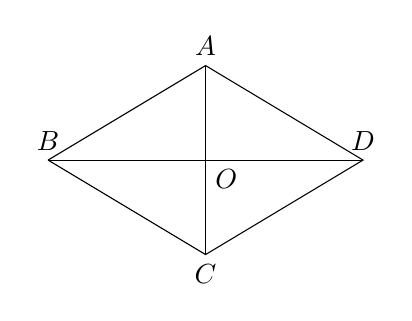
\begin{tikzpicture}
    \draw(-2,0)--(0,1.2)--(2,0)--(0,-1.2)--(-2,0);
    \draw(-2,0)node[above]{$B$}--(2,0)node[above]{$D$};
    \draw(0,1.2)node[above]{$A$}--(0,-1.2)node[below]{$C$};
    \node at (0,0)[below right]{$O$};        
    \end{tikzpicture}
    \caption{}
\end{figure}

求证:$AC$、$BD$互相垂直平分,且$AC$平分$\angle A$和$\angle C$,
$BD$平分$\angle B$和$\angle D$.
\end{example}

\begin{proof}
在四边形$ABCD$中,
因为$\overline{AB}=\overline{BC}=\overline{CD}=\overline{DA}$, 所
以四边形$ABCD$可看成由两个
等腰三角形所拼成:等腰$\triangle ABD$
与等腰$\triangle CBD$, 或等腰$\triangle ABC$
与等腰$\triangle ADC$. 由例3.8可知,
对角线$\overline{AC}$、$\overline{BD}$所在的直线都是四边形$ABCD$的对称
轴。所以,$\overline{AC}$、$\overline{BD}$互相垂直平分,并且$\overline{AC}$平分$\angle A$和
$\angle C$, $\overline{BD}$平分$\angle B$和$\angle D$.
\end{proof}

\begin{ex}
\begin{enumerate}
    \item 下列各图形有多少个对称轴?对称轴是什么?
    \begin{multicols}{3}
        \begin{enumerate}
            \item 线段;\item 射线;\item 直线。
        \end{enumerate}
    \end{multicols}
    \item 已知直线$\ell$和$\ell$外面一点$A$, 只用圆规和直尺求作点$A$以
    直线$\ell$为对称轴的对称点$A'$.
    \item 求作两个已知点的对称轴。
    \item 已知$\triangle ABC$和直线$\ell$, 作$\triangle ABC$以$\ell$为对称轴的对称形。
    \item 求作与已知等边三角形$ABC$分别以$AB$、$AC$、$BC$为对称
    轴的对称图形。
    \item 作图。(只要求作出图形)
    \begin{enumerate}
    \item 画已知线段$\overline{AB}$的对称轴。
    \item 画已知$\angle A$的对称轴。
    \end{enumerate}
    \item 等腰三角形有几个对称轴?等边三角形有几个对称轴?任
    画一个等边三角形把它的对称轴都画出来。
\end{enumerate}
\end{ex}

\subsection{三角形中的不等关系}
\begin{blk}{定义}
    和三角形的内角相邻并且和它互补的角叫做三角
形的\textbf{外角}。
\end{blk}
 
如图3.19中的$\angle ACD$
就是$\triangle ABC$的一外个角。
这时$\angle ACB$称为$\angle ACD$
相邻的内角,$\angle A$和$\angle B$
分别称为$\angle ACD$不相邻的内角。

\begin{blk}{定理}
 三角形的外角大于和它不相邻的任一内角。
\end{blk}

\begin{figure}[htp]\centering
    \begin{minipage}[t]{0.48\textwidth}
    \centering
\begin{tikzpicture}[>=latex, scale=1]
\draw(0,0)node[left]{$B$}--(4.5,0)node[right]{$D$};
\draw(3,0)node[below]{$C$}--(1.7,2)node[above]{$A$}--(0,0);
\draw(3.4,0) arc (0:120:.4);
    \end{tikzpicture}
    \caption{}
    \end{minipage}
    \begin{minipage}[t]{0.48\textwidth}
    \centering
    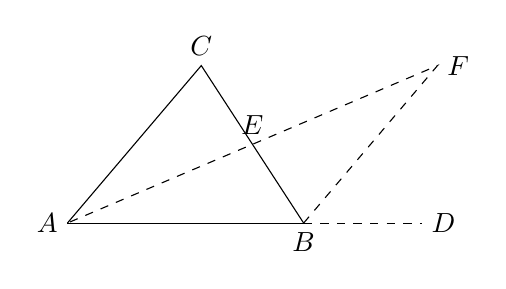
\begin{tikzpicture}[>=latex, scale=1]
\draw(0,0)node[left]{$A$}--(3,0)node[below]{$B$};
\draw[dashed](3,0)--(4.5,0)node[right]{$D$};
\draw(3,0)--(1.7,2)node[above]{$C$}--(0,0);
\draw[dashed](3,0)--(4.7,2)node[right]{$F$}--(0,0); 
\node at (2.35,1)[above]{$E$};
    \end{tikzpicture}
    \caption{}
    \end{minipage}
    \end{figure}

已知:$\triangle ABC$和外角
$\angle CBD$(图3.20)。

求证:$\angle CBD>\angle C$
或$\angle A$.

\begin{proof}
    假定$E$是$\overline{BC}$
中点,引$AE$并延长到$F$, 
使$\overline{EF}=\overline{AE}$, 作$\overline{BF}$.

在$\triangle ACE$和$\triangle FBE$中,

$\because\quad \overline{AE}=\overline{EF}$ (作图),

$\because\quad E$是$\overline{BC}$中点(假定),

$\therefore\quad \overline{CE}=\overline{EB}$(线段中点定义),

$\because\quad \angle CEA=\angle BEF$(对顶角相等),

$\therefore\quad \triangle ACE\cong \triangle FBE$ (SAS),

$\therefore\quad \angle EBF=\angle C$(全等三角形的对应角相等)。

由于$\angle CBD>\angle EBF$ (全量大于它的任何一部分)。

$\therefore\quad \angle CBD>\angle C$ (等量代换)。

同理可证 $\angle CBD> \angle A$.
\end{proof}

\begin{blk}{定理}
 在一个三角形中,如果两条边不等,那么它们所
对的角也不等,大边所对的角较大;反之,如果在一个三角
形中两个角不等,那么它们所对的边也不等。大角所对的边
较大。
\end{blk}

已知:$\triangle ABC$(图3.21)

\begin{figure}[htp]\centering
    \begin{minipage}[t]{0.48\textwidth}
    \centering
\begin{tikzpicture}[>=latex, scale=1.3]
\tkzDefPoint(0,0){A}
\tkzDefPoint(-50:2){C}
\tkzDefPoint(-120:2){D}
\tkzDefPoint(-120:3){B}
\tkzDefPoint(0,-1.5){O}
\tkzDrawPolygon(A,C,B)
\draw[dashed](D)--(C);
\tkzMarkAngles[mark=none, size=.3](C,D,A A,C,D)
\tkzLabelAngle[pos=.6](C,D,A){2}
\tkzLabelAngle[pos=.6](A,C,D){1}
\tkzAutoLabelPoints[center=O](A,C,B,D)       
    \end{tikzpicture}
    \caption{}
    \end{minipage}
    \begin{minipage}[t]{0.48\textwidth}
    \centering
    \begin{tikzpicture}[>=latex, scale=1.3]
\tkzDefPoint(0,0){A}
\tkzDefPoint(30:1.5){D}
\tkzDefPoint(-150:2){B}
\tkzDefPoint(-30:1.5){C}
\tkzDrawPolygon(A,C,B)
\draw[dashed](A)--(D)--(C);
\tkzMarkAngles[mark=none, size=.2](D,C,A A,D,C)
\tkzLabelAngle[pos=.4](A,D,C){2}
\tkzLabelAngle[pos=.4](D,C,A){1}
\tkzAutoLabelPoints[center=A](C,B,D)  
\node at (0,0)[above left]{$A$};
    \end{tikzpicture}
    \caption{}
    \end{minipage}
    \end{figure}

求证:
\begin{enumerate}
    \item $\overline{AB}>\overline{AC}\quad \Rightarrow\quad \angle C>\angle B$
    \item $\angle C>\angle B\quad \Rightarrow\quad \overline{AB}>\overline{AC}$
\end{enumerate}

\begin{proof}
    先证$\overline{AB}>\overline{AC}\quad\Rightarrow\quad \angle C>\angle B$.

在$AB$上截$\overline{AD}=\overline{AC}$,
则$\triangle ADC$为等腰三角形。

$\therefore\quad \angle 1=\angle 2$.

由于$\angle ACB>\angle 1$ (不等量基本性质6)

$\therefore\quad \angle ACB>\angle 2$(等量代换)。

但$\angle 2>\angle B$ (三角形的外角大于和它不相邻的任一内
角),

$\therefore\quad \angle ACB>\angle B$(不等量基本性质5)

即:$\angle C>\angle B$.

我们再证$\angle C>\angle B\quad \Rightarrow\quad \overline{AB}>\overline{AC}$

如果$\overline{AB}$不大于$\overline{AC}$, 那么$\overline{AB}=\overline{AC}$或$\overline{AB}<\overline{AC}$. 
若$\overline{AB}=\overline{AC}$, 则$\angle B=\angle C$, 若$\overline{AB}<\overline{AC}$,则$\angle C<\angle B$, 这两
种结果都和$\angle C>\angle B$矛盾。

$\therefore\quad \angle C>\angle B\quad \Rightarrow\quad \overline{AB}>\overline{AC}$
\end{proof}

\begin{blk}{定理}
    三角形任意两边之和大于第三边。
\end{blk}
 
已知:$\triangle ABC$(图3.23)。

求证:$\overline{AB}+\overline{AC}>\overline{BC}$.

\begin{proof}
    在$BA$的延长线上取一点$D$, 使$AD=AC$. 则
    $\triangle ACD$为等腰三角形。
  
    $\therefore\quad \angle 1=\angle 2$

    $\because\quad \angle BCD>\angle 1$(不等量
    基本性质6)

$\therefore\quad \angle BCD>\angle 2$(等量代
    换)。

    在$\triangle BCD$中,由前面的定理可知:
    $\overline{BD}>\overline{BC}$, 但$\overline{BD}=\overline{AB}+\overline{AD}=\overline{AB}+\overline{AC}$, 
 
   $\therefore\quad  \overline{AB}+\overline{AC}>\overline{BC}$
\end{proof}

\begin{blk}{推论}
三角形任一边大于其他两边之差。
\end{blk}

下面我们举例说明上述定理的一些应用。


\begin{example}
    已知:$\triangle ABC$中$\overline{AB}=\overline{AC}$, $D$点在$\overline{BC}$上,$E$点
在$\overline{BC}$的延长线上(图3.23)。

求证:$\overline{AD}<\overline{AB}<\overline{AE}$
\end{example}

\begin{figure}[htp]\centering
    \begin{minipage}[t]{0.48\textwidth}
    \centering
\begin{tikzpicture}[>=latex, scale=1]
    \tkzDefPoints{0/1.5/A, -1.5/-1/B, -.25/-1/D, 1.5/-1/C, 2.5/-1/E}
\tkzDrawPolygon(A,C,B)
    \draw(D)node[below]{$D$}--(A)node[above]{$A$}--(E)node[below]{$E$};
\draw[dashed](C)--(3.5,-1);
\node at (B)[below]{$B$};
\node at (C)[below]{$C$};
\tkzMarkAngles[mark=none, size=.3](D,B,A  A,D,B  A,C,B)
\tkzLabelAngle[pos=.5](D,B,A){1}
\tkzLabelAngle[pos=.5](A,D,B){3}
\tkzLabelAngle[pos=.5](A,C,B){2}
    \end{tikzpicture}
    \caption{}
    \end{minipage}
    \begin{minipage}[t]{0.48\textwidth}
    \centering
    \begin{tikzpicture}[>=latex, scale=1.2]
\tkzDefPoint(0,0){D}
\tkzDefPoint(-60:2){C}
\tkzDefPoint(180-60:1){A}
\tkzDefPoint(-140:1.2){E}
\tkzDefPoint(-140:2.8){B}
\tkzDrawPolygon(A,C,B)
\draw(B)--(E)--(C);
\draw[dashed](E)--(D);
\foreach \x in {A,D,C}
{
    \node at (\x) [right]{$\x$};
}
\foreach \x in {B,E}
{
    \node at (\x) [left]{$\x$};
}
\tkzMarkAngles[mark=none, size=.2](E,D,C)
\tkzLabelAngle[pos=.4](E,D,C){1}
    \end{tikzpicture}
    \caption{}
    \end{minipage}
    \end{figure}

\begin{proof}
$\because\quad \overline{AB}=\overline{AC}$

$\therefore\quad \angle 1=\angle 2$

又$\because\quad \angle 3>\angle 2$

$\therefore\quad \angle 3>\angle 1$

$\therefore\quad \overline{AB}>\overline{AD}$(在一个三角形中,大角对大边。)

又:$\because\quad \angle 2>\angle E$

$\therefore\quad \angle 1>\angle E$

$\therefore\quad \overline{AE}>\overline{AB}$(在一个三角形中,大角对大边。)

因此有:$\overline{AD}<\overline{AB}<\overline{AE}$
\end{proof}


\begin{example}
    已知:$E$点在$\triangle ABC$内(图3.24)。

求证: \begin{enumerate}
    \item $\angle BEC>\angle A$
    \item $\overline{BE}+\overline{EC}<\overline{AB}+\overline{AC}$
\end{enumerate} 
\end{example}

\begin{proof}
    延长$\overline{BE}$交$\overline{AC}$于$D$点,
则$\angle BEC>\angle 1$,$\angle BEC>\angle 1$

$\therefore\quad \angle BEC>\angle A$(不等量基
本性质5)。

又$\because\quad \overline{BE}+\overline{ED}<\overline{AD}+\overline{AB}$,$\overline{EC}<\overline{ED}+\overline{DC}$(三角形两边之和大于第三边)。

$\therefore\quad \overline{BE}+\overline{ED}+\overline{EC}<\overline{AD}+\overline{AB}+\overline{ED}+\overline{DC}$(不等量基本性质3)。

$\therefore\quad \overline{BE}+\overline{EC}<\overline{AB}+\overline{AC}$(不等量基本性质1)。
\end{proof}

\begin{example}
如图3.25所示,$A$、$B$是平面上直线$\ell$同侧的两点,
试在直线$\ell$上求一点$P$, 使$\overline{AP}+\overline{PB}$最短。

在没有作这题前,让我们想一想该怎样着手,我们要求
$\overline{AP}+\overline{PB}$最短,但怎样才能最短呢?

我们知道两点间的直线段最短,但是我们却要在$\ell$上求
一点,使$\overline{AP}+\overline{PB}$最短。如果$A,B$两点在$\ell$的两侧,那么问
题要简单得多(作$\overline{AB}$与$\ell$交于$P$, $P$点就是所求的点)。但
我们曾学过,如果两点是轴对称点,那么它们的对称轴就是
两点间线段的垂直平分线,并且对称轴上的点到两对称点的
距离相等。我们只要作出$A$点关于轴$\ell$的对称点$A'$, 我们求
$\overline{AP}+\overline{PB}$的最小值,就可转化为求$\overline{A'P}+\overline{PB}$的最小值了。
而$A'$、$B$两点在$\ell$的异侧,这是很容易的。

\begin{figure}[htp]
    \centering
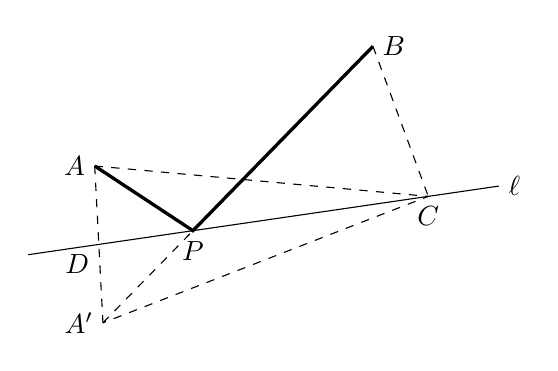
\begin{tikzpicture}[xscale=.6, rotate=5]
\draw (-2,0)--(8,0)node[right]{$\ell$};
\draw[dashed](-.5,1)node[left]{$A$}--(-.5,-1)node[left]{$A'$};
\draw[dashed](-.5,-1)--(5.5,2)node[right]{$B$};
\draw[very thick](-.5,1)--(1.5,0)node[below]{$P$}--(5.5,2);
\node at (-.5,0)[below left]{$D$};
\draw[dashed](-.5,1)  -- (6.5,0) node[below]{$C$}--(-.5,-1);
\draw[dashed](5.5,2)  -- (6.5,0);
\end{tikzpicture}
    \caption{}
\end{figure}
\end{example}


\begin{solution}
    作$A$点关于轴$\ell$的对称点$A'$, 作$\overline{A'B}$与$\ell$相交于$P$, 
    则$P$点使$\overline{AP}+\overline{PB}$最短。因为,如果在$\ell$上任找另外一点$C$, 
    在$\triangle A'BC$中,
    $\overline{A'B}<\overline{A'C}+\overline{CB}$(三角形两边之和大于第三边),
    但$\overline{A'B}=\overline{A'P}+\overline{PB}$

将    $\overline{A'P}=\overline{AP},\quad \overline{A'C}=\overline{AC}$ 代入上式,
    则得:$\overline{AP}+\overline{PB}<\overline{AC}+\overline{CB}$.

    这就证明了$P$点使$\overline{AP}+\overline{PB}$最短。
\end{solution}

\begin{rmk}
    如果$\ell$是镜子的话,那么从$A$点发出的光线,若反
射到$B$点,那么$\overline{AP}$、$\overline{PB}$就是光所走的路线。因为光线总是
走最近的路,在光学中就有:“入射角等于反射角”这条定
律。即$\angle APD=\angle BPC$. 在光学中由观测得到的结果和我
们用数学定理得出的结果一致。在自然界中我们有能力观测
到的结论是有限的,如何由这些有限的可观测的结论,得到
更进一步的结论,甚至有些是观测不到的结论,我们需要数
学这样有力的工具。
\end{rmk}
    
\begin{ex}
\begin{enumerate}
    \item 已知:如图,$\triangle ABC$内有一点$P$, 
    求证:$\angle BPC>\angle BAC$.
    \item 已知:如图,$\triangle ABC$内有一点P,
    求证:$\overline{AB}+\overline{AC}>\overline{PB}+\overline{PC}$.
    \item 将金属丝弯成三角形,如果要求一边长是25cm, 那么
    金属丝至少大于多少cm才能作成三角形?
    \item 证明四边形两条对角线之和小于周长而大于半周长。
 \item 证明三角形的一边小于它的周长的一半。
 \item  用整数表示三角形的各边,一边是3米,另一边是2米,第
    三边可以是多少米?
\item  在平面上$\overline{AB}$
    的垂直平分线的$A$点的一侧取一点$P$, 那
    么$\overline{PA}$和$\overline{PB}$哪一条线段长?
\item 已知:如图,$\triangle ABC$中,
$\angle A>\angle C$, $D$、$E$分别在$\overline{AB}$、
    $\overline{AC}$上并且$\overline{AD}>\overline{AE}$.
    求证:
    \begin{enumerate}
        \item $\angle BDE> \angle CED$
        \item $\overline{BC}>\overline{BE}$
    \end{enumerate}
\end{enumerate}
\end{ex}
    
\begin{figure}[htp]\centering
    \begin{minipage}[t]{0.48\textwidth}
    \centering
\begin{tikzpicture}[>=latex, scale=1]
    \tkzDefPoint(-60:2){C}
    \tkzDefPoint(180-60:1){A}
    \tkzDefPoint(-140:2.8){B}
    \tkzDefPoint(-.25,-.5){P}
    \tkzDrawPolygon(A,C,B)
    \draw(B)--(P)--(C);
\tkzAutoLabelPoints[center=P](A,B,C)
\node at (P)[above]{$P$};
    \end{tikzpicture}
    \caption*{第1--2题}
    \end{minipage}
    \begin{minipage}[t]{0.48\textwidth}
    \centering
    \begin{tikzpicture}[>=latex, scale=1.3]
        \tkzDefPoint(0,0){A}
        \tkzDefPoint(-45:2){C}
        \tkzDefPoint(-45:1){E}
        \tkzDefPoint(-140:2.8){B}
        \tkzDefPoint(-140:2){D}
        \tkzDrawPolygon(A,C,B)
        \tkzDrawPolygon(D,B,E)
        \tkzDefPoint(.1,-1){O}
        \tkzAutoLabelPoints[center=O](A,B,C,D,E)

    \end{tikzpicture}
    \caption*{第8题}
    \end{minipage}
    \end{figure}

\subsection*{习题3.1}

\begin{enumerate}
    \item 已知:如图,$\overline{AD}=\overline{AE}$, $\overline{BD}=\overline{EC}$, 
    求证:$\overline{DO}=\overline{EO}$.
    \item 已知:如图,$\overline{AB}=\overline{AD}$, $AC$平分$\angle BAD$, $E$是$\overline{AC}$上一点。
    求证:$\angle EBC=\angle EDC$.
    \item 求证:等腰三角形两腰上的中线相等。
    \item 已知:如图,$\angle B=\angle C$, $\overline{BD}=\overline{EC}$. 
    求证:$\angle 1=\angle 2$.

\begin{figure}[htp]\centering
    \begin{minipage}[t]{0.31\textwidth}
    \centering
\begin{tikzpicture}[>=latex, scale=1]
\tkzDefPoints{-1.5/0/B, 1.5/0/C, -.5/2/D, .5/2/E, 0/3/A}
\tkzDrawPolygon(A,B,C)
\tkzDrawSegments(B,E C,D)
\tkzInterLL(C,D)(B,E)  \tkzGetPoint{O}
\tkzLabelPoints[left](B,D)
\tkzLabelPoints[right](C,E)
\tkzLabelPoints[above](A)
\tkzLabelPoints[below](O)


    \end{tikzpicture}
    \caption*{第1题}
    \end{minipage}
    \begin{minipage}[t]{0.31\textwidth}
    \centering
    \begin{tikzpicture}[>=latex, scale=1]
\tkzDefPoints{-1.5/0/B, 1.5/0/D, 0/1.5/A, 0/-2/C, 0/.8/E}
\tkzDrawPolygon(A,B,C,D)
\tkzDrawSegments(B,E A,C E,D)
\tkzLabelPoints[left](B)
\tkzLabelPoints[right](D)
\tkzLabelPoints[above](A)
\tkzLabelPoints[below](C)
\tkzLabelPoints[below right](E)
    \end{tikzpicture}
    \caption*{第2题}
    \end{minipage}
        \begin{minipage}[t]{0.31\textwidth}
    \centering
    \begin{tikzpicture}[>=latex, scale=1]
\tkzDefPoints{-1.5/0/B, 1.5/0/C, -.75/0/D, .75/0/E, 0/3/A}
\tkzDrawPolygon(A,B,C)
\tkzDrawSegments(A,E A,D)
\tkzLabelPoints[left](B)
\tkzLabelPoints[right](C)
\tkzLabelPoints[above](A)
\tkzLabelPoints[below](D,E)
\tkzMarkAngles[mark=none, size=.3](C,D,A A,E,B)
\tkzLabelAngle[pos=.5](C,D,A){1}
\tkzLabelAngle[pos=.5](A,E,B){2}
    \end{tikzpicture}
    \caption*{第4题}
    \end{minipage}
    \end{figure}

    \item 已知:如图,在四边形$ABCD$中,
    $\overline{AD}=\overline{AB}$, $\overline{CD}=\overline{BC}$
    
    求证:$\angle 1=\angle 2$;$\angle 3=\angle 4$;$AC\bot DB$
  
    \item 如图,已知:$\angle 1=\angle 2$, $\angle 3=\angle 4$, 
求证:$\overline{AB}=\overline{AC}$.
\item 如图,已知:$\overline{BE}=\overline{ED}$, $\angle 1=\angle 2$.
求证:$\overline{AB}=\overline{CD}$.

\begin{figure}[htp]\centering
    \begin{minipage}[t]{0.48\textwidth}
    \centering
\begin{tikzpicture}[>=latex, scale=1]
    \tkzDefPoints{-2/0/A, 2/0/C, -1/1.5/D, -1/-1.5/B, -1/0/E}
    \tkzDrawPolygon(A,B,C,D)
    \tkzLabelPoints[left](A)
    \tkzLabelPoints[right](C)
    \tkzLabelPoints[above](D)
    \tkzLabelPoints[below](B)
    \tkzLabelPoints[above right](E)
    \tkzDrawSegments(A,C D,B)
    \tkzMarkAngles[mark=none, size=.4](C,A,D D,C,A)
    \tkzMarkAngles[mark=none, size=.5](B,A,C A,C,B)
    \tkzLabelAngle[pos=.7](C,A,D){1}
    \tkzLabelAngle[pos=.7](B,A,C){2}
    \tkzLabelAngle[pos=.7](D,C,A){3}
    \tkzLabelAngle[pos=.7](A,C,B){4}

    \end{tikzpicture}
    \caption*{第5题}
    \end{minipage}
    \begin{minipage}[t]{0.48\textwidth}
    \centering
    \begin{tikzpicture}[>=latex, scale=1]
        \tkzDefPoints{-1.5/0/B, 1.5/0/C, 0/3.5/A, 0/1/O}
        \tkzDrawPolygon(A,B,C)
        \tkzLabelPoints[left](B)
        \tkzLabelPoints[right](C)
        \tkzLabelPoints[above](A)
        \tkzLabelPoints[below](O)
        \tkzDrawSegments(A,O B,O C,O)        
        \tkzMarkAngles[mark=none, size=.4](C,B,O O,C,B)
        \tkzMarkAngles[mark=none, size=.3](A,O,B)
        \tkzLabelAngle[pos=.6](C,B,O){1}
        \tkzLabelAngle[pos=.6](O,C,B){2}
        \tkzLabelAngle[pos=.5](A,O,B){3}
        \tkzMarkAngles[mark=none, size=.35](C,O,A)
        \tkzLabelAngle[pos=.5](C,O,A){4}

    \end{tikzpicture}
    \caption*{第6题}
    \end{minipage}
    \end{figure}

\item 在$\triangle ABC$中,$\overline{AB}=\overline{AC}$, $D$、$E$
两点分别在$\overline{AB}$和$\overline{AC}$上,且$\overline{BE}$
和$\overline{CD}$交于$O$点,$\overline{BD}=\overline{CE}$. 求证:$AO$平分$\angle BAC$.
\item 在$\triangle ABC$中,$D$为$\overline{BC}$延长线上一点,且$\overline{CD}=\overline{AC}$, $F$
是
$\overline{AD}$中点,$\overline{CE}$是$\angle ACB$的平分线。求证$CE\bot CF$.

\item 在$\triangle ABC$中,$\angle B=2\angle C$, $AD$平分$\angle A$, 交$\overline{BC}$于$D$点,
求证:$\overline{AB}+\overline{BD}=\overline{AC}$.

\begin{figure}[htp]\centering
    \begin{minipage}[t]{0.48\textwidth}
    \centering
\begin{tikzpicture}[>=latex, scale=1]
    \tkzDefPoints{-1.5/0/A, 1.5/0/C, -1/2/B, 1/2/D}
    \tkzDrawPolygon(A,B,C)
    \tkzDrawPolygon(A,D,C)
    \tkzInterLL(B,C)(A,D) \tkzGetPoint{E}
    \tkzLabelPoints[left](A)
    \tkzLabelPoints[right](C)
    \tkzLabelPoints[above](B,D,E)
 
    \tkzMarkAngles[mark=none, size=.4](B,C,A C,A,D)
    \tkzLabelAngle[pos=.6](C,A,D){1}
    \tkzLabelAngle[pos=.6](B,C,A){2}

    \end{tikzpicture}
    \caption*{第7题}
    \end{minipage}
    \begin{minipage}[t]{0.48\textwidth}
    \centering
    \begin{tikzpicture}[>=latex, scale=1]
\tkzDefPoints{0/0/B, 3/0/C, 3/1.5/D}
\tkzDefPoint(70:3){A}
\tkzDrawPolygon(A,B,C,D)
\tkzLabelPoints[below](B,C)
\tkzLabelPoints[above](A,D)
    \end{tikzpicture}
    \caption*{第11题}
    \end{minipage}
    \end{figure}

\item 如图,已知四边形$ABCD$中,
$\overline{AB}=\overline{BC}$, $\overline{AD}>\overline{CD}$. 

求证:$\angle BCD>\angle BAD$.
\item 已知:$\triangle ABC$中,$D$是$\overline{AC}$上
一点,且$\overline{BD}>\overline{BC}$. 

求证:$\overline{AB}>\overline{AC}$.
\item 三角形的一边等于2米,另一边等于8米,如果已知第三
边能用被3整除的整数表示,求第三边。
\item 已知:$\triangle ABC$在平面$\alpha$上,点$P\in\alpha$, 并且$P$在$\triangle ABC$
的外部

求证:$\overline{PA}+\overline{PB}+\overline{PC}>\frac{1}{2}(\overline{AB}+\overline{BC}+\overline{AC})$
\item 已知:$\triangle ABC$在平面$\alpha$上,点$P\in\alpha$, 并且$P$在$\triangle ABC$
的内部

求证:$\overline{PA}+\overline{PB}+\overline{PC}<\overline{AB}+\overline{BC}+\overline{AC}$.
\item 求证:三角形一边上的中线小于其他两边和的一半。
\item 在两条公路$OX$和$OY$上,分别设邮筒$A$和$B$, 邮递员每
天由邮局$P$到邮筒$A$、$B$取信,然后返回邮局。问$A$、$B$的
位置确定在哪儿,才能使邮递员走的路程最短?

\begin{figure}[htbp]
    \centering
\begin{tikzpicture}
\tkzDefPoints{-2/0/X, 2/0/Y, .5/3/X1, -.5/3/Y1, 0/0/P}
\tkzDefPointWith[linear, K=.5](X,X1) \tkzGetPoint{A}
\tkzDefPointWith[linear, K=.3](Y,Y1) \tkzGetPoint{B}
\tkzDrawPolygon(A,B,P)
\tkzInterLL(X,X1)(Y,Y1)  \tkzGetPoint{O}
\tkzDrawSegments(X,X1 Y,Y1)
\tkzLabelPoints[below](X,Y,P)
\tkzLabelPoints[left](A)
\tkzLabelPoints[right](B,O)
\end{tikzpicture}
    \caption*{第17题}
\end{figure}
\end{enumerate}

\section{平行线与内角和定理}

\subsection{平行线}
\begin{blk}
    {定义}
平面上两条直线被第三条直线所截,截得八个
角,如图3.26, 其中的$\angle 1$和$\angle 5$, $\angle 4$和$\angle 8$, $\angle 2$和$\angle 6$, 
$\angle 3$和$\angle 7$, 都叫做\textbf{同位角},$\angle 4$和$\angle 6$, $\angle 3$和$\angle 5$都叫\textbf{内错
角},$\angle 4$和$\angle 5$, $\angle 3$和$\angle 6$都叫做\textbf{同旁内角}。
\end{blk}

\begin{figure}[htp]\centering
    \begin{minipage}[t]{0.48\textwidth}
    \centering
\begin{tikzpicture}[>=latex, scale=1]
\tkzDefPoints{-2/2/A, 2/2.5/B, -2/0/C, 2/1.5/D, 0/-.5/F, 0/4/E}
\tkzDrawSegments(A,B C,D E,F)
\tkzInterLL(A,B)(E,F)  \tkzGetPoint{P}
\tkzInterLL(C,D)(E,F)  \tkzGetPoint{Q}
\tkzMarkAngles[mark=none, size=.4](B,P,E A,P,F D,Q,E C,Q,F)
\tkzLabelAngle[pos=.6](B,P,E){1}
\tkzLabelAngle[pos=.6](A,P,F){3}
\tkzLabelAngle[pos=.6](D,Q,E){5}
\tkzLabelAngle[pos=.6](C,Q,F){7}
\tkzMarkAngles[mark=none, size=.3](E,P,A F,P,B E,Q,C F,Q,D)
\tkzLabelAngle[pos=.5](E,P,A){2}
\tkzLabelAngle[pos=.5](F,P,B){4}
\tkzLabelAngle[pos=.5](E,Q,C){6}
\tkzLabelAngle[pos=.5](F,Q,D){8}
    \end{tikzpicture}
    \caption{}
    \end{minipage}
    \begin{minipage}[t]{0.48\textwidth}
    \centering
    \begin{tikzpicture}[>=latex, scale=1]
\tkzDefPoints{-2/2/A, 2/2/B, -2/0/C, 2/0/D, -1/-1/F, 1/3/E}
\tkzDrawSegments(A,B C,D E,F)
\tkzInterLL(A,B)(E,F)  \tkzGetPoint{P}
\tkzInterLL(C,D)(E,F)  \tkzGetPoint{Q}
\tkzMarkAngles[mark=none, size=.4](B,P,E A,P,F)
\tkzLabelAngle[pos=.6](B,P,E){4}
\tkzLabelAngle[pos=.6](A,P,F){3}
\tkzLabelAngle[pos=.6](D,Q,E){2}
\tkzMarkAngles[mark=none, size=.3](F,P,B D,Q,E)
\tkzLabelAngle[pos=.5](F,P,B){1}
\tkzLabelPoints[above](A,B,C,D)
\tkzLabelPoints[below](Q)
\tkzLabelPoints[above left](P)
    \end{tikzpicture}
    \caption{}
    \end{minipage}
    \end{figure}


由平行线定义可知,两条直线平行的充要条件是这两条
直线被第三条直线所截出的同位角相等。这就是说:
\begin{enumerate}
\item 如
果同位角相等,则两条直线平行;   
\item 如果已知两条直线平
行,则同位角相等。 
\end{enumerate}
这就是平行线的判定方法和平行线的性
质。以此为根据又可推知以下定理:

\begin{blk}{定理}
两条直线被第三条直所线截,如果
内错角相等,或同旁内角互补,那么这两条
直线平行。
\end{blk}

\begin{proof}
   在图3.27中,设直线$AB$、$CD$被直线$PQ$所截。
$\angle 2$、$\angle 3$是内错角,$\angle 1$、$\angle 2$是同旁内角。
\begin{enumerate}
    \item 如果已知$\angle 2=\angle 3$. 

$\because\quad \angle 3=\angle 4$    (对顶角相等),

$\therefore\quad \angle 2=\angle 4$(等量代换)。

$\therefore\quad AB\parallel CD$(同位角相等,则两条直线平行)。

\item 如果已知$\angle 1+\angle 2=180^{\circ}$, 
则$\angle 2=180^{\circ}-\angle 1$(等量减等量差相等)。

$\because\quad PQ$是直线(已知)

$\therefore\quad \angle 4+\angle 1=180^{\circ}$.

$\therefore\quad \angle 4=180^{\circ}-\angle 1$.

$\therefore\quad \angle 2=\angle 4$(等量代换)。

$\therefore\quad AB\parallel CD$(同位角相等,则两条直线平行)。  
\end{enumerate}
\end{proof}

\begin{blk}{定理} 
    平面上两条不相交的直线是这两条直线互相平行
的充要条件。
\end{blk}


但是这个定理的证明比较麻烦,我们在这里就不证了,
有兴趣的同学可以自己去证明它。

\begin{blk}
   {推论1} 平行于同一直线的两条直线平行。 
\end{blk}

已知:直线$a\parallel$直线$c$, 直线$b\parallel$直线$c$ (图3.28).
 求证:$a\parallel b$.

\begin{proof}
    若$a$不平行$b$, $a$与$b$一定相交,设交点为$P$, 那么
过$P$点就有两条直线$a$、$b$平行于直线$c$, 但根据平行公理,
这是不可能的,所以$a\parallel b$.
\end{proof}

\begin{figure}[htp]
    \centering
\begin{tikzpicture}
\begin{scope}
    \foreach \x/\xtext in {0/c,1/b,2/a}
    {
        \draw(0,\x)--node[above]{$\xtext$}(3,\x);
    }
\end{scope}
\begin{scope}[xshift=5cm]
    \foreach \x/\xtext in {0/c,1/b,2/a}
    {
        \draw(0,\x)--node[above]{$\xtext$}(3,\x);
    }
\draw[dashed](3,1)--(4.5,1.5)node[right]{$P$}--(3,2);
\end{scope}
\end{tikzpicture}
    \caption{}
\end{figure}


上面这种证明方法,叫做反证法。我们先否定要证明的
结论,然后引出不合理的结果,从而说明结论非成立不可。
请同学们回想一下,我们在第二章讲基本逻辑语句的命题
时,若原命题是“若$\alpha$, 则$\beta$”,那么它的逆否命题是“若
非$\beta$, 则非$\alpha$.”我们知道这两个互为逆否的命题是同义
的,上面的反证法就是当我们证明原命题有困难时,我们可
去证它的逆否命题。

\begin{blk}
 {推论2} 过已知直线外一点,只可以引一条直线和已知
直线垂直。   
\end{blk}

请同学们用反证法证明这个推论。

\begin{example}
已知:在图3.29中,$\angle BED=\angle B+\angle D$.

求证:$AB\parallel CD$.
\end{example}

\begin{analyze}
    若能证明$AB$、$CD$都
与第三条直线平行,则$AB\parallel CD$.
\end{analyze}

\begin{proof}
    引直线$EF$, 使得$\angle 1=\angle B$, 则$AB\parallel EF$(内错角相等,则两条直线平行)。

又:$\because\quad \angle BED=\angle B+\angle D$(已知),

$\therefore\quad \angle BED-\angle 1=\angle D$(等量减等量差相等)。
即:$\angle FED=\angle D$.

$\therefore\quad CD\parallel EF$ (内错角相等,则两条直线平行)。

$\therefore\quad AB\parallel CD$ (平行于第三条直线的两条直线平
行)。
\end{proof}

\begin{figure}[htp]\centering
    \begin{minipage}[t]{0.48\textwidth}
    \centering
\begin{tikzpicture}[>=latex, scale=1]
\tkzDefPoints{0/0/C, 3/0/D, 2/1/E, 3/2/B, 0/2/A, 4/1/F}
\tkzDrawSegments(C,D D,E E,B A,B)
\tkzDrawSegments[dashed](E,F)
\tkzLabelPoints[below](C,D)
\tkzLabelPoints[above](A,B)
\tkzLabelPoints[left](E)
\tkzLabelPoints[right](F)
\tkzMarkAngles[mark=none, size=.4](F,E,B)
\tkzLabelAngle[pos=.6](F,E,B){1}

    \end{tikzpicture}
    \caption{}
    \end{minipage}
    \begin{minipage}[t]{0.48\textwidth}
    \centering
    \begin{tikzpicture}[>=latex, scale=1]
\tkzDefPoints{-.25/-.25/B, .25/.25/C, 1/-.25/F, -1/.25/E, 1.5/1.5/D, -1.5/-1.5/A}
\tkzDrawPolygon(A,E,C)
\tkzDrawPolygon(B,F,D)
\tkzLabelPoints[below](A,B,F)
\tkzLabelPoints[above](E,D,C)
\tkzMarkAngles[mark=none, size=.4](F,B,D E,C,A)
\tkzLabelAngle[pos=.6](F,B,D){2}
\tkzLabelAngle[pos=.6](E,C,A){1}

    \end{tikzpicture}
    \caption{}
    \end{minipage}
    \end{figure}

\begin{example}
    在图3.30中,已知$\overline{CD}=\overline{AB}$, $AD$是直线。
$\angle A=\angle D$, 并且$\overline{AE}=\overline{DE}$.

求证:$EC\parallel BF$.

\end{example}

\begin{analyze}
要证$EC\parallel BF$, 只需证明$\angle 1=\angle 2$即可,要证明
$\angle 1=\angle 2$, 只需证明$\triangle AEC\cong \triangle DFB$即可。
\end{analyze}

\begin{proof}
    $\because\quad \overline{AB}=\overline{CD}$(已知)
    $\therefore\quad \overline{AB}+\overline{BC}=\overline{BC}+\overline{CD}$(等量加等量和相等)。即:$\overline{AC}=\overline{BD}$.

又:$\because\quad \angle A=\angle D,\quad \overline{AE}=\overline{DF}$(已知),

$\therefore\quad \triangle AEC\cong \triangle DFB$ (SAS).

$\therefore\quad \angle 1=\angle 2$(全等三角形的对应角相等)。

$\therefore\quad CE\parallel BF$(内错角相等,则两条直线平行)。
\end{proof}

\begin{blk}
  {定理} 如果两条平行直线被一条直线所截,那么截出的
内错角相等;同旁内角互补。  
\end{blk}

这个定理同学们可以根据“两条直线平行则同位角相
等”这一性质推出。

\begin{example}
     在图3.31中,
已知:$OA\parallel O'A'$, $OB\parallel O'B'$.

求证:$\angle AOB=\angle A'O'B'$.   
\end{example}

\begin{proof}
    反向延长$O'A'$交$OB$于$C$点,

$\because\quad OB\parallel O'B'$(已知),

$\therefore\quad\angle A'O'B'=\angle A'CB$(两条直线平行,同位角相等)。

又$\because\quad OA\parallel O'A'$(已知),

$\therefore\quad \angle A'CB=\angle AOB$(两条直线平行,同位角相等)。

$\therefore\quad \angle AOB=\angle A'O'B'$(等量代换)。
\end{proof}

\begin{figure}[htp]\centering
    \begin{minipage}[t]{0.48\textwidth}
    \centering
\begin{tikzpicture}[>=latex, scale=1, rotate=-20]
\tkzDefPoints{0/0/O, 4/0/A, 2.5/1.5/O', 4.5/1.5/A', 0/1.5/C', 2.5+1.414/1.5+1.414/B', 2.5/2.5/B, 1.5/1.5/C}
\tkzDrawSegments(A,O A',O' B,O B',O')
\tkzDrawSegments[dashed](O',C')
\tkzLabelPoints[below](O,A,O',A')
\tkzLabelPoints[above](C,B,B')

    \end{tikzpicture}
    \caption{}
    \end{minipage}
    \begin{minipage}[t]{0.48\textwidth}
    \centering
    \begin{tikzpicture}[>=latex, scale=1]
\tkzDefPoints{0/0/B, 3/0/C, 1/2/A, 4/2/D}
\tkzDrawPolygon(A,B,C,D)
\tkzDrawSegments(A,C)
\tkzLabelPoints[left](A,B)\tkzLabelPoints[right](C,D)

\tkzMarkAngles[mark=none, size=.4](A,C,B C,A,D)
\tkzMarkAngles[mark=none, size=.3](B,A,C D,C,A)
\tkzLabelAngle[pos=.6](A,C,B){2}
\tkzLabelAngle[pos=.6](C,A,D){1}
\tkzLabelAngle[pos=.5](B,A,C){3}
\tkzLabelAngle[pos=.5](D,C,A){4}
    \end{tikzpicture}
    \caption{}
    \end{minipage}
    \end{figure}

上面的例子我们可以写成下面的定理:

\begin{blk}
    {定理} 如果一个角的两条边和另一个角的两条边分别同
向平行,那么这两个角相等。
\end{blk}

\begin{example}
    图3.32中,
    已知:$AD\parallel BC$, $\overline{AD}=\overline{BC}$.

    求证:$AB\parallel CD$.
\end{example}

\begin{analyze}
    要证明$AB\parallel CD$, 只要证明$\angle 3=\angle 4$就行
了,为此需要证明$\triangle ABC\cong \triangle CDA$.
\end{analyze}

\begin{proof}
$\because\quad AD\parallel BC$(已知),

$\therefore\quad \angle 1=\angle 2$(两条直线平行,则
内错角相等)。

又:$\because\quad \overline{AD}=\overline{BC}$(已知)
$\overline{AC}=\overline{AC}$(公共边)

$\therefore\quad \triangle ABC\cong \triangle CDA$ (SAS)

$\therefore\quad \angle  3=\angle 4$(全等三角形的对应角相等)。

$\therefore\quad AB\parallel CD$(内错角相等,则两条直线平行)。
\end{proof}

\begin{ex}
\begin{enumerate}
    \item 指出图中用数字标出的角中哪些是同位角?
    \item 如图,说出下列各对角的名称。
    $\angle 1$与$\angle 2$, $\angle 2$与$\angle 3$, $\angle 3$与$\angle 4$, $\angle 4$与$\angle 5$, $\angle 3$与
    $\angle 5$,$\angle 1$与$\angle 6$
    \item 试指出判定两条直线平行有哪些方法?并指出平行线
    有什么性质?
    \item 如图,已知:$\angle 1=60^{\circ}$, $\angle 2=60^{\circ}$. 
    求证:$AB\parallel CD$.

    \item 如图,已知:$\angle 1=\angle 2$, 求证:$AB\parallel CD$.
    \item 知图,已知$\angle 1=69^{\circ}$, $\angle 2=69^{\circ}$.
    求证:$AB\parallel CD$.
    \item 如图,已知:$\angle 1+\angle 2=180^{\circ}$, 求证:$AB\parallel CD$.
    \item 如图,已知:$\overline{AB}$、$\overline{CD}$相交于$E$点,且$\overline{EA}=\overline{EB}$, $\overline{EC}=\overline{ED}$
    
求证:$AC\parallel DB$.

\item 如图,已知:$\overline{AB}=\overline{DC}$, $\overline{AD}=\overline{BC}$. 求证:$AB\parallel CD$.
\item 已知:$\overline{AE}=\overline{DF}$, $\overline{AB}=\overline{CD}$, $\overline{EC}=\overline{BF}$. 
求证:$EC\parallel BF$.
\item 已知:$DE\parallel BC$, $\angle 1=\angle 2$. 求证:$\angle 3=\angle 4$.
\item 已知:$AB\parallel CD$, 求证:$\angle 1=\angle 2$.
\item 如图,已如:$\angle 1=\angle 2$. 求证:$\angle 3=\angle 4$.
\item 如图,已知:$AB\parallel CD$, 
求证:$\angle B+\angle D+\angle E=360^{\circ}$.

\item 在四边形$ABCD$中,$AD\parallel BC$, $AB\parallel CD$且$\overline{BE}=\overline{DF}$, 则$\overline{AE}\parallel \overline{FC}$.
\end{enumerate}
\end{ex}

\begin{figure}[htp]\centering
    \begin{minipage}[t]{0.48\textwidth}
    \centering
\begin{tikzpicture}[>=latex, scale=1]
\tkzDefPoints{0/0/A, 4/1/B, 0/1.5/C, 4/2.5/D, 2/-.5/F, 2/3.5/E}
\tkzDrawSegments(A,B C,D E,F)
\tkzInterLL(A,B)(E,F)  \tkzGetPoint{X1}
\tkzInterLL(C,D)(E,F)  \tkzGetPoint{X2}
\tkzDefPoints{3.5/2/Y1, 3.5/3.5/Y2}
\tkzDrawSegments(X1,Y1 X2,Y2)
\tkzMarkAngles[mark=none, size=.45](B,X1,Y1 D,X2,Y2)
\tkzLabelAngle[pos=.6](B,X1,Y1){4}  \tkzLabelAngle[pos=.6](D,X2,Y2){3}
\tkzMarkAngles[mark=none, size=.35](Y1,X1,E Y2,X2,E)
\tkzLabelAngle[pos=.6](Y1,X1,E){2}  \tkzLabelAngle[pos=.6](Y2,X2,E){1}
    \end{tikzpicture}
    \caption*{第1题}
    \end{minipage}
    \begin{minipage}[t]{0.48\textwidth}
    \centering
    \begin{tikzpicture}[>=latex, scale=1]
 \tkzDefPoints{0/0/A, 4/.8/B, 1.5/-1/C, 4/-.5/D, 0/2.5/E, 1.5/2.5/F}
 \tkzDrawSegments(A,B C,D A,E C,F)
 \tkzInterLL(A,B)(C,F)  \tkzGetPoint{G}     
 \tkzMarkAngles[mark=none, size=.3](B,A,E D,C,F B,G,F A,G,C)
 \tkzLabelAngle[pos=.5](B,A,E){1}  \tkzLabelAngle[pos=.5](D,C,F){4}
 \tkzLabelAngle[pos=.5](B,G,F){2} \tkzLabelAngle[pos=.5](A,G,C){3}
 \tkzMarkAngles[mark=none, size=.25](C,G,B F,G,A)
 \tkzLabelAngle[pos=.4](C,G,B){5}  \tkzLabelAngle[pos=.4](F,G,A){6}
    \end{tikzpicture}
    \caption*{第2题}
    \end{minipage}
    \end{figure}



\begin{figure}[htp]\centering
    \begin{minipage}[t]{0.32\textwidth}
    \centering
\begin{tikzpicture}[>=latex, scale=1]
    \tkzDefPoints{0/0/C, 2.5/0/D, 0/1/A, 2.5/1/B, .5/-1/E, 2.25/2.25/F}
\tkzInterLL(A,B)(E,F) \tkzGetPoint{X1}
\tkzInterLL(C,D)(E,F) \tkzGetPoint{X2}
\tkzLabelPoints[left](A,C)\tkzLabelPoints[right](B,D)
\tkzDrawSegments(A,B C,D E,F)
\tkzMarkAngles[mark=none, size=.4](A,X1,E C,X2,E)
\tkzLabelAngle[pos=.6](A,X1,E){1}  \tkzLabelAngle[pos=.6](C,X2,E){2}
    \end{tikzpicture}
    \caption*{第4题}
    \end{minipage}
    \begin{minipage}[t]{0.32\textwidth}
    \centering
    \begin{tikzpicture}[>=latex, scale=1]
\tkzDefPoints{0/0/C, 2.5/0/D, 0/1/A, 2.5/1/B, .5/-1/E, 2.25/2.25/F}
\tkzInterLL(A,B)(E,F) \tkzGetPoint{X1}
\tkzInterLL(C,D)(E,F) \tkzGetPoint{X2}
\tkzLabelPoints[left](A,C)\tkzLabelPoints[right](B,D)
\tkzDrawSegments(A,B C,D E,F)
\tkzMarkAngles[mark=none, size=.4](B,X1,F C,X2,E)
\tkzLabelAngle[pos=.6](B,X1,F){1}  \tkzLabelAngle[pos=.6](C,X2,E){2}
    \end{tikzpicture}
    \caption*{第5、7、12题}
    \end{minipage}
    \begin{minipage}[t]{0.32\textwidth}
    \centering
    \begin{tikzpicture}[>=latex, scale=1]
 \tkzDefPoints{0/0/C, 2.5/0/D, 0/1/A, 2.5/1/B, .5/-1/E, 2.25/2.25/F}
\tkzInterLL(A,B)(E,F) \tkzGetPoint{X1}
\tkzInterLL(C,D)(E,F) \tkzGetPoint{X2}
\tkzLabelPoints[left](A,C)\tkzLabelPoints[right](B,D)
\tkzDrawSegments(A,B C,D E,F)
\tkzMarkAngles[mark=none, size=.4](B,X1,F E,X2,D)
\tkzLabelAngle[pos=.6](B,X1,F){1}  \tkzLabelAngle[pos=.6](E,X2,D){2}
    \end{tikzpicture}
    \caption*{第6题}
    \end{minipage}
    \end{figure}

\begin{figure}[htp]\centering
    \begin{minipage}[t]{0.32\textwidth}
    \centering
\begin{tikzpicture}[>=latex, scale=1]
\tkzDefPoints{0/0/D, 2.5/0/B, -.5/1.5/A, 2/1.5/C}
\tkzInterLL(A,B)(C,D) \tkzGetPoint{E}
\tkzDrawPolygon(A,C,E)
\tkzDrawPolygon(B,D,E)
\tkzLabelPoints[above](A,C)
\tkzLabelPoints[below](B,D,E)
    \end{tikzpicture}
    \caption*{第8题}
    \end{minipage}
    \begin{minipage}[t]{0.32\textwidth}
    \centering
    \begin{tikzpicture}[>=latex, scale=1]
\tkzDefPoints{0/0/B, 2.5/0/C, .75/1.5/A, 3.25/1.5/D}
\tkzDrawPolygon(A,B,C,D)
\tkzLabelPoints[above](A,D)
\tkzLabelPoints[below](B,C)
    \end{tikzpicture}
    \caption*{第9题}
    \end{minipage}
    \begin{minipage}[t]{0.32\textwidth}
        \centering
        \begin{tikzpicture}[>=latex, scale=1]
\tkzDefPoints{0/0/A, 1/0/B,2/0/C,3/0/D, .5/1/E, 2.5/-1/F}
\tkzDrawPolygon(A,C,E)
\tkzDrawPolygon(B,D,F)
\tkzLabelPoints[above](E,D)
\tkzLabelPoints[below](A,B,C,F)
        \end{tikzpicture}
        \caption*{第10题}
        \end{minipage}
    \end{figure}



    \begin{figure}[htp]\centering
        \begin{minipage}[t]{0.46\textwidth}
        \centering
    \begin{tikzpicture}[>=latex, scale=.8]
\tkzDefPoints{0/0/B, 4/0/C, 2.2/4/A}
\tkzDefPointWith[linear, K=.6](A,B) \tkzGetPoint{D}
\tkzDefPointWith[linear, K=.6](A,C) \tkzGetPoint{E}
\tkzDrawPolygon(A,B,C)
\tkzDrawSegments(D,E)
\tkzLabelPoints[left](B,D)
\tkzLabelPoints[right](C,E)
\tkzLabelPoints[above](A)
\tkzMarkAngles[mark=none, size=.4](E,D,A C,B,A A,C,B A,E,D)
\tkzLabelAngle[pos=.6](E,D,A){3}  \tkzLabelAngle[pos=.6](C,B,A){1}
\tkzLabelAngle[pos=.6](A,C,B){2}  \tkzLabelAngle[pos=.6](A,E,D){4}
        \end{tikzpicture}
        \caption*{第11题}
        \end{minipage}
        \begin{minipage}[t]{0.46\textwidth}
        \centering
        \begin{tikzpicture}[>=latex, scale=1]
 \tkzDefPoints{0/0/C, 3/0/D, 0/1/A, 3/1/B, .5/-1/E, 1.5/2/F, 2.5/-1/G, 2/2/H}
 \tkzDrawSegments(A,B C,D E,F G,H)
\tkzLabelPoints[left](A,C)\tkzLabelPoints[right](B,D)
\tkzInterLL(A,B)(E,F) \tkzGetPoint{X1}
\tkzInterLL(C,D)(E,F) \tkzGetPoint{X2}
\tkzInterLL(A,B)(G,H) \tkzGetPoint{Y1}
\tkzInterLL(C,D)(G,H) \tkzGetPoint{Y2}

\tkzMarkAngles[mark=none, size=.25](A,X1,E D,X2,F G,Y1,B G,Y2,D)
\tkzLabelAngle[pos=.4](G,Y1,B){3}  \tkzLabelAngle[pos=.4](A,X1,E){1}
\tkzLabelAngle[pos=.4](D,X2,F){2}  \tkzLabelAngle[pos=.4](G,Y2,D){4}


        \end{tikzpicture}
        \caption*{第13题}
        \end{minipage}

        \end{figure}

    \begin{figure}[htp]\centering
        \begin{minipage}[t]{0.46\textwidth}
        \centering
    \begin{tikzpicture}[>=latex, scale=1]
\tkzDefPoints{0/0/C, 2.5/0/D, 0/1.5/A, 3/1.5/B, 4/1/E}
\tkzLabelPoints[above](A,B)
\tkzLabelPoints[below](C,D)
\tkzLabelPoints[right](E)
\tkzDrawSegments(A,B C,D D,E B,E)
        \end{tikzpicture}
        \caption*{第14题}
        \end{minipage}
        \begin{minipage}[t]{0.46\textwidth}
            \centering
            \begin{tikzpicture}[>=latex, scale=1]
\tkzDefPoints{0/0/D, 3/0/A, 0.75/2/C, 3.75/2/B}
\tkzLabelPoints[right](A,B)
\tkzLabelPoints[left](C,D)
\tkzDrawSegments(B,D)
\tkzDrawPolygon(A,B,C,D)
\tkzDefPointWith[linear, K=.3](B,D) \tkzGetPoint{E}
\tkzDefPointWith[linear, K=.7](B,D) \tkzGetPoint{F}
\tkzDrawSegments(A,E C,F)
\tkzLabelPoints[below](F)
\tkzLabelPoints[above](E)
            \end{tikzpicture}
            \caption*{第15题}
            \end{minipage}
        \end{figure}



\subsection{内角和定理}

\begin{blk}
  {三角形内角和定理} 三角形三内角和等于$180^{\circ}$.  
\end{blk}

这个定理在第一章用实验的办法验证过,现在我们应用
平行线的性质来证明它。

已知:任一$\triangle ABC$(图3.33). 求证:$\angle A+\angle B+
\angle C=180^{\circ}$.

\begin{figure}[htp]
    \centering
\begin{tikzpicture}
\tkzDefPoints{0/0/B, 4/0/C, 1/2.5/A, 0/2.5/D, 4/2.5/E}
\tkzDrawPolygon(A,C,B)
\tkzDrawSegments[dashed](D,E)
\tkzLabelPoints[left](B,D)\tkzLabelPoints[right](C,E)
\tkzLabelPoints[above](A)
\end{tikzpicture}
    \caption{}
\end{figure}

\begin{proof}
    过$A$点引直线
$DE\parallel BC$(平行公理)
则$\angle DAB=\angle B$, $\angle EAC=\angle C$(两条直线平行,
则内错角相等)。

$\because\quad DE$是过$A$点的直线(作图),

$\therefore\quad \angle DAB+\angle BAC+\angle CAE=180^{\circ}$(平角定义)。

$\therefore\quad \angle A+\angle B+\angle C=180^{\circ}$(等量代换)。
\end{proof}

由三角形内角和定理可以得到下列推论。

\begin{blk}
    {推论1} 一个三角形的两角若分别等于另一个三角形的
两角,则第三个角也相等。
\end{blk}


\begin{blk}
    {推论2} 两个三角形如果有两个角和其中一个角所对的
边分别相等,那么它们就全等。(AAS)
\end{blk}


\begin{blk}
    {推论3} 三角形的一个外角等于和它不相邻的两个内角
的和。
\end{blk}

\begin{blk}
    {推论4} 正三角形的各内角是$60^{\circ}$.
\end{blk}

\begin{blk}
    {推论5 }三角形中,至多有一个直角或一个钝角。
\end{blk}

\begin{blk}
   {定义} 每个内角都是锐角的三角形,叫做\textbf{锐角三角形};
有一个内角是直角的三角形叫做\textbf{直角三角形},夹直角的两边
叫做\textbf{直角边},直角的对边叫做\textbf{斜边};有一个内角是钝角的三
角形叫做\textbf{钝角三形角}(图3.34)。
\end{blk}

\begin{figure}[htp]
    \centering
\begin{tikzpicture}
\begin{scope}
    \tkzDefPoints{0/0/A, 3/0/B, 1.6/3/C}
    \tkzDrawPolygon(A,B,C)
\tkzMarkAngles[mark=none, size=.4](B,A,C C,B,A A,C,B)
\node at (1.5,-.5){锐角三角形};
\end{scope}
\begin{scope}[xshift=4cm]
        \tkzDefPoints{0/0/A, 2/0/B, 2/3/C}
    \tkzDrawPolygon(A,B,C)
    \node at (1,-.5){直角三角形};
    \tkzMarkRightAngles(C,B,A)
\end{scope}
\begin{scope}[xshift=7cm]
    \tkzDefPoints{0/0/A, 2/0/B, 3.6/2.8/C}
    \tkzDrawPolygon(A,B,C)
    \tkzMarkAngles[mark=none, size=.3](C,B,A)
    \node at (1.8,-.5){钝角三角形};
\end{scope}
\end{tikzpicture}
    \caption{}
\end{figure}

这样,三角形可以根据它的内角的大小分为三类:锐角
三角形、直角三角形和钝角三角形。

\begin{blk}
{推论6} 直角三角形中,非直角的两个角都是锐角,并
且这两个锐角互余。
\end{blk}

\begin{blk}
{定义}
三边都不相等的三角形叫做\textbf{不等边三角形}。
\end{blk}

这样三角形又可以按边长分成三类:等边三角形,底边
和腰不等的等腰三角形和不等边三角形。


\begin{example}
    已知:$O$是$\triangle ABC$内任一点(图3.35)。

求证:$\angle BOC=\angle A+\angle ABO+\angle ACO$.
\end{example}

\begin{proof}
 引$AO$交$\overline{BC}$于$D$点,
则$\angle DOB=\angle ABO+\angle BAO$, 
$\angle DOC=\angle ACO+\angle CAO$(三
角形外角等于不相邻内角和)

$\therefore\quad \angle DOB+\angle DOC=\angle ABO+\angle ACO+
\angle BAO+\angle CAO$(等量加等量和相等)。

$\therefore\quad \angle BOC=\angle A+\angle ABO+\angle ACO$
\end{proof}

\begin{figure}[htp]\centering
    \begin{minipage}[t]{0.48\textwidth}
    \centering
\begin{tikzpicture}[>=latex, scale=1]
\tkzDefPoints{0/0/B, 3/0/C, 2.5/3/A, 2/1.2/O}
\tkzDrawPolygon(A,B,C)
\tkzDrawSegments(B,O O,C)
\tkzInterLL(A,O)(B,C) \tkzGetPoint{D}
\tkzDrawSegments[dashed](A,D)
\tkzLabelPoints[below](B,D,C)
\tkzLabelPoints[above](A,O)
    \end{tikzpicture}
    \caption{}
    \end{minipage}
    \begin{minipage}[t]{0.48\textwidth}
    \centering
    \begin{tikzpicture}[>=latex, scale=1]
\tkzDefPoints{-1.5/0/B, 1.5/0/C, 0/3.2/A}
\tkzDrawPolygon(A,B,C)
\tkzDefPointBy[projection = onto A--B](C) \tkzGetPoint{D}
\tkzDefPointBy[projection = onto A--C](B) \tkzGetPoint{E}
\tkzDrawSegments(B,E C,D)
\tkzLabelPoints[left](D,B)
\tkzLabelPoints[right](E,C)
\tkzLabelPoints[above](A)
\tkzMarkRightAngles[size=.2](B,D,C C,E,B)


    \end{tikzpicture}
    \caption{}
    \end{minipage}
    \end{figure}


\begin{example}
    在图3.36中。
    已知:$\overline{CD}\bot\overline{AB}$于$D$, $\overline{BE}\bot\overline{AC}$于$E$, 且$\overline{BE}=\overline{CD}$.

    求证:$\angle ABC=\angle ACB$
\end{example}

\begin{proof}
    在$\triangle ABE$与$\triangle ACD$中,

$\because\quad  \overline{BE}\bot\overline{AC}$于$E$. $\overline{CD}\bot\overline{AB}$于$D$(已知)

$\therefore\quad \angle ADC=90^{\circ},\quad \angle AEB=90^{\circ}$
(垂直定义)。

$\therefore\quad \angle ADC=\angle AEB$(等量代换)。

又$\because\quad \angle A=\angle A$(公共角),$\overline{BE}=\overline{CD}$(已知)

$\therefore\quad \triangle ABE\cong \triangle ACD$ (AAS).

$\therefore\quad \overline{AB}=\overline{AC}$(全等三角形的对应边相等)。

$\therefore\quad \angle ABC=\angle ACB$. (等腰三角形的两底角相等)。
\end{proof}

\begin{example}
    试证明定理:角平分线上的点与角的两边距离
相等。

已知:$BD$是$\angle ABC$的平分线,$P\in BD$, $\overline{PE}\bot BA$于
$E$, $\overline{PF}\bot BC$于$F$ (图3.37). 
求证:$\overline{PE}=\overline{PF}$.
\end{example}

\begin{figure}[htp]
    \centering
\begin{tikzpicture}
\tkzDefPoints{0/0/B, 4/0/D, 3/0/P}
\tkzDefPoint(25:3.8){A}  \tkzDefPoint(-25:3.8){C}
\tkzDefPointBy[projection = onto A--B](P) \tkzGetPoint{E}
\tkzDefPointBy[projection = onto B--C](P) \tkzGetPoint{F}
\tkzMarkRightAngles[size=.2](B,E,P B,F,P)
\tkzDrawSegments(A,B B,C B,D E,P F,P)
\tkzLabelPoints[below](F,C,P) \tkzLabelPoints[above](E,A)
\tkzLabelPoints[left](B)\tkzLabelPoints[right](D)
\end{tikzpicture}
    \caption{}
\end{figure}

\begin{proof}
在$\triangle PEB$和$\triangle PFB$中,

$\because\quad BD$平分$\angle ABC$(已知),

$\therefore\quad \angle EBP=\angle FBP$(角平分线定义)。

又$\because\quad \overline{PE}\bot BA$于$E$, 
$\overline{PF}\bot BC$于$F$(已知),

$\therefore\quad \angle PEB=90^{\circ}$, $\angle PFB=90^{\circ}$(垂直定义),

$\therefore\quad \angle PEB=\angle PFB$(等量代换)。

又$\because\quad \overline{BP}=\overline{BP}$(公共边),

$\therefore\quad \triangle PEB\cong \triangle PFB$ (AAS)

$\therefore\quad \overline{PE}=\overline{PF}$(全等三角形的对应边相等)。
\end{proof}

\begin{blk}
    {定义} 连结多边形的不相邻两个顶点的线段叫做这个多
    边形的\textbf{对角线}。如图3.38中的四边形$ABCD$中就有两条对
    角线$\overline{AC}$、$\overline{BD}$.
\end{blk}

\begin{figure}[htp]\centering
    \begin{minipage}[t]{0.48\textwidth}
    \centering
\begin{tikzpicture}[>=latex, scale=1]
\tkzDefPoints{0/0/B, 3/.5/C, 2.8/1.8/D, 1.3/2.5/A}
\tkzDrawPolygon(A,B,C,D)
\tkzDrawSegments(A,C B,D)
\tkzLabelPoints[below](B,C)
\tkzLabelPoints[above](A,D)
    \end{tikzpicture}
    \caption{}
    \end{minipage}
    \begin{minipage}[t]{0.48\textwidth}
    \centering
    \begin{tikzpicture}[>=latex, scale=1]
        \tkzDefPoints{0/0/C, 1.7/.5/D, 2.5/1.5/E, 1/2.5/A, -.75/1.3/B}
        \tkzDrawPolygon(A,B,C,D,E)
        \tkzDrawSegments(A,C A,D)
        \tkzLabelPoints[left](B,C) \tkzLabelPoints[right](E,D)
        \tkzLabelPoints[above](A)
    \end{tikzpicture}
    \caption{}
    \end{minipage}
    \end{figure}

\begin{blk}
    {推论}
从$n$边形的一个顶点引对角线,可把这个$n$边形分
成$n-2$个三角形,如图3.39中的五边形$ABCDE$,从$A$点
引对角线$\overline{AC}$、$\overline{AD}$,则分成了三个三角形。
\end{blk}

由此推论不难得出多边形内角和定理:

\begin{blk}{多边形内角和定理}
    任意$n$边形的内角和等于$(n-2)\x180^{\circ}$.  
\end{blk}

这个定理请同学们参看图3.40或图3.41自己证明。

\begin{figure}[htp]\centering
    \begin{minipage}[t]{0.48\textwidth}
    \centering
\begin{tikzpicture}[>=latex, scale=1]
\tkzDefPoint(-20:1.5){A_4}
\tkzDefPoint(40:1.5){A}
\tkzDefPoint(80:1.5){B}
\tkzDefPoint(-60:1.5){A_3}
\tkzDefPoint(-130:1.5){A_2}
\tkzDefPoint(180:1.5){A_1}
\tkzDefPoint(130:1.5){A_n}
\tkzDrawSegments(A_1,A A_1,A_4 A_1,A_3)
\tkzDrawPolygon(A_1,A_2,A_3,A_4,A,B,A_n)
\tkzDefPoint(0,0){O}
\tkzAutoLabelPoints[center=O](A_1,A_2,A_3,A_4,A_n)


    \end{tikzpicture}
    \caption{}
    \end{minipage}
    \begin{minipage}[t]{0.48\textwidth}
    \centering
    \begin{tikzpicture}[>=latex, scale=1]
\tkzDefPoint(-20:1.5){A}
\tkzDefPoint(80:1.5){A_4}
\tkzDefPoint(-60:1.75){A_n}
\tkzDefPoint(-130:1.4){A_1}
\tkzDefPoint(170:1.5){A_2}
\tkzDefPoint(130:1.25){A_3}
\tkzDrawSegments(O,A_1 O,A_2 O,A_3 O,A_4 O,A_n O,A)
\tkzDrawPolygon(A_1,A_2,A_3,A_4,A,A_n)
\tkzDefPoint(0,0){O}
\tkzAutoLabelPoints[center=O](A_1,A_2,A_3,A_4,A_n)
\draw(0,0) circle(.5);
\tkzLabelPoints[below](O)

    \end{tikzpicture}
    \caption{}
    \end{minipage}
    \end{figure}

\begin{blk}{定义}
    多边形内角的一边和另一边的反向延长线所组
成的角叫做多边形的\textbf{外角}。
\end{blk}

对于任一个$n$边形每一内角取一个相应的外角,如图3.42中的$\alpha'_1, \alpha'_2,\ldots,\alpha'_n$, 很显然,一个内角与它相应的一个外角和为一个平角,因此:
\[\begin{split}
  (n-2)  \text{个平角外角和}+\text{外角和}&=\text{内角和}+\text{外角和}\\
  &=(\alpha_1+\alpha_2+\cdots+\alpha_n)+(\alpha'_1+\alpha'_2+\cdots+\alpha_n')\\
  &=n\text{个平角}
\end{split}\]
$\therefore\quad \text{外角和}=\text{2个平角}=360^{\circ}$

因而有多边形外角和定
理:

\begin{blk}{多边形外角和定理}
  任意多边形外角和都等
于$360^{\circ}$  
\end{blk}


\begin{blk}
  {定义} 各边都相等,各
角都相等的多边形叫做\textbf{正多
边形}。  
\end{blk}

\begin{figure}[htp]\centering
    \begin{minipage}[t]{0.48\textwidth}
    \centering
\begin{tikzpicture}[>=latex, scale=1]
\tkzDefPoint(20:1.5){B}
\tkzDefPoint(20+60:1.5){C}
\tkzDefPoint(20+120:1.5){D}
\tkzDefPoint(20+180:1.5){E}
\tkzDefPoint(20+240:1.5){F}
\tkzDefPoint(-40:1.5){A}
\tkzDrawPolygon(A,B,C,D,E,F)
\tkzDefPointWith[linear, K=1.75](A,B)  \tkzGetPoint{B1}
\tkzDefPointWith[linear, K=1.75](B,C)\tkzGetPoint{C1}
\tkzDefPointWith[linear, K=1.75](C,D)\tkzGetPoint{D1}
\tkzDefPointWith[linear, K=1.75](D,E)\tkzGetPoint{E1}
\tkzDefPointWith[linear, K=1.75](E,F)\tkzGetPoint{F1}
\tkzDefPointWith[linear, K=1.75](F,A)\tkzGetPoint{A1}

\tkzDrawSegments(A,A1 B,B1 C,C1 D,D1 E,E1 F,F1)
\tkzMarkAngles[mark=none, size=.4](B1,B,C1 C1,C,D1 D1,D,E1 E1,E,F1 F1,F,A A1,A,B1)
\tkzMarkAngles[mark=none, size=.25](F,E,D E,D,C D,C,B C,B,A B,A,F A,F,E)

\tkzLabelAngle[pos=.5](F,E,D){$\alpha_1$}
\tkzLabelAngle[pos=.5](A,F,E){$\alpha_2$}
\tkzLabelAngle[pos=.5](B,A,F){$\alpha_3$}
\tkzLabelAngle[pos=.5](C,B,A){$\alpha_4$}
\tkzLabelAngle[pos=.5](E,D,C){$\alpha_n$}
\tkzLabelAngle[pos=.7](E1,E,F1){$\alpha_1'$}
\tkzLabelAngle[pos=.7](F1,F,A){$\alpha_2'$}
\tkzLabelAngle[pos=.7](A1,A,B1){$\alpha_3'$}
\tkzLabelAngle[pos=.7](B1,B,C1){$\alpha_4'$}
\tkzLabelAngle[pos=.7](D1,D,E1){$\alpha_n'$}
    \end{tikzpicture}
    \caption{}
    \end{minipage}
    \begin{minipage}[t]{0.48\textwidth}
    \centering
    \begin{tikzpicture}[>=latex, scale=1]
\tkzDefPoint(180-18:2){B}
\tkzDefPoint(-126:2){C}
\tkzDefPoint(-54:2){D}
\tkzDefPoint(18:2){E}
\tkzDefPoint(90:2){A}
\tkzDrawPolygon(A,B,C,D,E)
\tkzDefPoint(0,0){O}
\tkzAutoLabelPoints[center=O](A,B,C,D,E)
\tkzDrawSegments(A,D C,E)
\tkzInterLL(A,D)(C,E)  \tkzGetPoint{F}
\tkzLabelPoints[left](F)
\tkzMarkAngles[mark=none, size=.4](F,A,E  E,D,F F,E,D)
\tkzMarkAngles[mark=none, size=.3](E,F,A A,E,F)
\tkzLabelAngle[pos=.7](E,D,F){$36^{\circ}$}
\tkzLabelAngle[pos=.7](F,E,D){$36^{\circ}$}
\tkzLabelAngle[pos=.6](A,E,F){$72^{\circ}$}
\tkzLabelAngle[pos=.7](F,A,E){$36^{\circ}$}
\node at (54:1.8){$a$};
    \end{tikzpicture}
    \caption{}
    \end{minipage}
    \end{figure}


\begin{example}
    在图3.43中,已知:$ABCDE$是正五边形,对角
    线$\overline{AD}$、$\overline{CE}$相交于$F$.

    求证:$\triangle AEF$、$\triangle DEF$、$\triangle CDF$都是等腰三角形。
\end{example}

\begin{proof}
由多边形内角和公式可知:正五边形的各内角
和
\[(5-2)\x180^{\circ}=540^{\circ}\]
由于正五边形各内角相等,

$\therefore\quad \angle AED=540^{\circ}\x\frac{1}{5}=108^{\circ}$

$\because\quad \triangle EAD$是等腰三角形,

$\therefore\quad \angle EAD=\angle EDA=(180^{\circ}-108^{\circ})\x\frac{1}{2}=36^{\circ}$

$\because\quad \triangle DCE$也是等腰三角形,
$\angle D=108^{\circ}$,

$\therefore\quad \angle DEF=36^{\circ}$.

$\therefore\quad \angle AEF=108^{\circ}-36^{\circ}=72^{\circ}$

$\angle AFE=180^{\circ}-36^{\circ}-72^{\circ}=72^{\circ}$, $\overline{AE}=\overline{AF}$.

$\therefore\quad \triangle AEF$是等腰三角形。

同理可证$\triangle CDF$也是等腰三角形,腰长等于正五边形的
边长;$\triangle DEF$也是等腰三角形。

请同学们用量角器和直尺,
划一个正五边形。
\end{proof}
    
\begin{example}
    已知:正六边形
    $ABCDEF$ (图3.44)。

    求证:对角线$\overline{AD}$、$\overline{BE}$
    $\overline{CF}$相交于一点,且把正六
    边形$ABCDEF$分割成六个
    正三角形。
\end{example}

\begin{figure}[htp]
    \centering
\begin{tikzpicture}
\tkzDefPoint(20:2){E}
\tkzDefPoint(80:2){F}
\tkzDefPoint(140:2){A}
\tkzDefPoint(200:2){B}
\tkzDefPoint(260:2){C}
\tkzDefPoint(320:2){D}
\tkzDefPoint(0,0){O}
\tkzAutoLabelPoints[center=O](A,B,C,D,E,F)
\tkzDrawSegments(A,D B,E C,F)
\tkzDrawPolygon(A,B,C,D,E,F)
\tkzLabelPoints[above right](O)
\end{tikzpicture}
    \caption{}
\end{figure}

\begin{proof}
    已知$ABCDEF$是正六边形,所以它的每一
    个内角
    \[(6-2)\x180^{\circ} \x\frac{1}{6}=120^{\circ}\]
    
    以$\overline{AB}$为边作正三角形$ABO$, 顶点$O$在正六边形$ABCD
    EF$内,连结$\overline{OC}$、$\overline{OD}$、$\overline{OE}$、$\overline{OF}$.

$\because\quad \angle B=120^{\circ},\quad \angle ABO=60^{\circ}$,
 
$\therefore\quad \angle OBC=60^{\circ}$.

又$\because\quad \overline{OB}=\overline{BC}$,

$\therefore\quad \angle BCO=\angle BOC=60^{\circ}$.

$\therefore\quad \triangle OBC$也是正三角形。

    同理可证:
$\triangle OCD$、$\triangle ODE$、$\triangle OEF$、$\triangle OFA$都是正三角形。
    由于$\angle AOB+\angle BOC+\angle COD=180^{\circ}$, 所以$A$、$O$、$D$
    在同一条直线上,同理,$B$、$O$、$E$,$C$、$O$、$F$也都分别在
    同一条直线上,所以对角线$\overline{AD}$、$\overline{BE}$、$\overline{CF}$相交于一点$O$, 
    且把正六边形分隔成六个全等的正三角形。
\end{proof}


    根据例3.21得出的正六边形的性质,请同学们想想,若已知
    正六边形的边长,如何用圆规和直尺画一个正六边形。
    


\begin{example}
    测量斜面的倾斜角,常用测倾仪(图3.45(1))。
测倾仪悬垂的指针所指的度数,就是倾角的度数,为什么?
\begin{figure}[htp]
    \centering
\includegraphics[scale=.6]{fig/3-45.png}
    \caption{}
\end{figure}
\end{example}


\begin{analyze}
    为了便于说明,我们将测倾仪指针所指倾角和斜面
    的斜角位置关系用图3.45(2)来表示,问题便转化为:

    已知:$AC\bot BC$, $AD\bot BD$. 求证:$\angle A=\angle B$.
\end{analyze}

\begin{proof}
    设$BC$、$AD$相交于$E$点。

$\because\quad AC\bot BC$  (已知),

$\therefore\quad \angle ECA=90^{\circ}$ (垂直定义)。

$\therefore\quad$ 在$\triangle ACE$中,$\angle A+\angle AEC=90^{\circ}$(直角三角形两锐角互余)。

同理:$\angle B+\angle BED=90^{\circ}$

又$\because\quad \angle AEC=\angle BED$(对顶角相等),

$\therefore\quad \angle A=\angle B$(等角的余角相等)。
\end{proof}
这个例题可以写成下面的定理:

\begin{blk}
   {定理} 如果一个锐角的两边分别垂直于另一个锐角的两
边,那么这两个锐角相等。 
\end{blk}

根据这个定理很容易证明下面的例题。

\begin{example}
已知:在图3.46中,
$\angle BAC=90^{\circ}$, $AD\bot BC$于
$D$点。

求证:$\angle B=\angle CAD$, $\angle C=\angle BAD$.
\end{example}


\begin{proof}
$\because\quad $在$\triangle ABC$中,
$\angle BAC=90^{\circ}$(已知),

$\therefore\quad \angle B$、$\angle C$都是锐角(直角三角形中,非直角的两
个角都是锐角)。

又$\because\quad AD$在$\angle BAC$的内部,

$\therefore\quad \angle CAD$也是锐角(全量大于它的任何一部分)。

由于,$AB\bot AC$, $AD\bot BC$, 

$\therefore\quad \angle B=\angle CAD$.

同理:$\angle C=\angle BAD$.(两边分别互相垂直的两个锐角相
等)
\end{proof}

\begin{figure}[htp]\centering
    \begin{minipage}[t]{0.48\textwidth}
    \centering
\begin{tikzpicture}[>=latex, scale=1]
\tkzDefPoints{0/0/B, 3.2/0/D, 5/0/C, 3.2/2.4/A}
\tkzDrawPolygon(A,B,C)
\tkzDrawSegments(A,D)
\tkzLabelPoints[below](B,C,D)
\tkzLabelPoints[above](A)
\tkzMarkAngles[mark=none, size=.3](C,B,A)
\tkzMarkRightAngles(A,D,C B,A,C)

    \end{tikzpicture}
    \caption{}
    \end{minipage}
    \begin{minipage}[t]{0.48\textwidth}
    \centering
    \begin{tikzpicture}[>=latex, scale=1]
\tkzDefPoints{-1.5/0/B, 1.5/0/B', 0/0/C, 0/2.5/A}
\tkzDrawPolygon(A,B,B')
\tkzDrawSegments(A,C)
\tkzMarkRightAngles(A,C,B)
\tkzLabelPoints[below](B,B')
\node at (C)[below]{$C(C')$};
\node at (A)[above]{$A(A')$};
    \end{tikzpicture}
    \caption{}
    \end{minipage}
    \end{figure}


\begin{example}
    已知:$\triangle ABC$和$\triangle A'B'C'$中,
$\angle ACB=\angle A'C'B'=90^{\circ}$, $\overline{AB}=\overline{A'B'}$,
$\overline{AC}=\overline{A'C'}$ (图3.47).

求证:$\triangle ABC\cong \triangle A'B'C'$
\end{example}

\begin{proof}
    根据移形公理,移动
$\triangle A'B'C'$, 因$\overline{AC}=\overline{A'C'}$,
所以可使$\overline{A'C'}$与$\overline{AC}$重合,
并使$B$、$B'$落于$\overline{AC}$的两侧。

由于$\angle ACB=\angle ACB'=90^{\circ}$.

$\therefore\quad \angle  BCB'=180^{\circ}$.

$\therefore\quad B$、$C$、$B'$在一条直线上。

在$\triangle ABB'$中,

$\because\quad \overline{AB}=\overline{A'B}=\overline{AB'}$,

$\therefore\quad \angle B=\angle B'$(等腰三角形的两底角相等)。

在$\triangle ABC$和$\triangle A'B'C'$中,

$\because\quad \angle ACB=\angle A'C'B'$, $\angle B=\angle B'$, $\overline{AB}=\overline{A'B'}$.

$\therefore\quad \triangle ABC\cong \triangle A'B'C'$ (AAS)    
\end{proof}

由上例可得如下定理:

\begin{blk}
  {定理} 斜边和一直角边对应相等的两个直角三角形全
等。  
\end{blk}

\begin{ex}
\begin{enumerate}
    \item 求下列各图中的$\angle x$、$\angle y$的度数。
    \item 如果等腰$\triangle ABC$的顶角是$\angle C$, 
\begin{enumerate}
\item 当$\angle C=40^{\circ}$ 时,求$\angle A$;
\item 当$\angle C=m^{\circ}$ 时,求$\angle B$;
\item 当$\angle A=40^{\circ}$ 时,求$\angle C$;
\item 当$\angle B=n^{\circ}$ 时,求$\angle C$.
\end{enumerate}

\item 已知$\triangle ABC$中,$\overline{AB}=\overline{AC}$, $AD$是$\angle BAC$的外角平分
    线,求证$AD\parallel BC$.
    \item 求证:三角形的两个外角的和减去第三个内角等于二个
    直角。
    \item 试证:若三角形的二外角和等于三个直角,此三角形必
    是直角三角形。
    \item 如果等腰三角形的顶角是$60^{\circ}$, 则此三角形为正三角
    形。
    \item 在$\triangle ABC$中,$\angle A=25^{\circ}$, $\angle B=68^{\circ}$, 经过这个三角
    形的顶点,作对边的平行线,求这些直线组成的三角形的
    三内角的度数。
    \item 三角形的两个角分别等于$62^{\circ}$ 和$72^{\circ}$, 从这两个角的顶
    点作
    对边的高线,求这两条高线的夹角。
    \item 如果一个三角形的任意两个角的和大于$90^{\circ}$, 这个三角
    形是怎样的三角形?
\item 已知六边形$ABCDEF$中,
$\angle A=a^{\circ}$, $\angle B=b^{\circ}$, 
$AF\parallel CD$, $AB\parallel DE$, 试
求图中$x$、$y$的度数。
\item 求七边形与十边形的内
角和。
\item 如果多边形的所有内角和等于:
\[1080^{\circ} ,\quad 1620^{\circ}  ,\quad 3960^{\circ}  ,\quad 1840^{\circ}\]那
么这些多边形各有几条边?
\item 如果多边形的每一个内角都等于:
\[144^{\circ} ,\quad 150^{\circ}  ,\quad 170^{\circ}  ,\quad 111^{\circ} 
,\quad 190^{\circ}\] 
那么这些多边形各有几条边?
\item 试证:两条平行线被一条直线所截时,两同旁内角的平
分线互相垂直。
\item 设$\overline{CD}$和$\overline{AE}$是$\triangle ABC$的高,求证$\angle BCD=\angle BAE$.
\item 试证:等腰三角形两腰上的高线相等。
\item 试证:等腰三角形中,从底的中点到两腰的距离相
等。
\item 试证:与角的两边距离相等的点在该角的平分线上。
\item 试证:与线段两端点距离相等的点在该线段的垂直平分
线上。
\end{enumerate}
\end{ex}

\begin{figure}[htp]
    \centering
\begin{tikzpicture}
\begin{scope}
\tkzDefPoints{0/0/B, 5/0/C, 3.5/3.5/A, 2.5/1.5/D}
\tkzDrawPolygon(A,B,C)
\tkzDrawSegments(B,D C,D)
\tkzMarkAngles[mark=none, size=.4](A,C,D B,A,C B,D,C)
\tkzMarkAngles[mark=none, size=1.2](D,B,A)
\tkzLabelAngle[pos=1.6](D,B,A){$23^{\circ}$}
\tkzLabelAngle[pos=.6](A,C,D){$39^{\circ}$}
\tkzLabelAngle[pos=.6](B,A,C){$70^{\circ}$}
\tkzLabelAngle[pos=.6](B,D,C){$x$}
\tkzLabelPoints[below](B,C)
\tkzLabelPoints[above](A)

\end{scope}
\begin{scope}[xshift=6cm, yshift=1cm]
    \tkzDefPoints{0/0/B, 4/-1/C, 0/1/A, 3/2.5/E, 4.5/1/D}
    \tkzDrawPolygon(A,B,C,D,E)
    \tkzLabelPoints[below](B,C)
    \tkzLabelPoints[above](E)
    \tkzLabelPoints[right](D)
    \tkzLabelPoints[left](A)
    \tkzMarkAngles[mark=none, size=.3](C,B,A B,A,E A,E,D E,D,C)
\tkzMarkRightAngle(D,C,B)
\tkzLabelAngle[pos=.6](C,B,A){$105^{\circ}$}
\tkzLabelAngle[pos=.6](A,E,D){$120^{\circ}$}
\tkzLabelAngle[pos=.6](B,A,E){$x$}
\tkzLabelAngle[pos=.6](E,D,C){$107^{\circ}$}
\tkzDefPointWith[linear, K=1.8](E,D) \tkzGetPoint{F}
\tkzDrawSegments[dashed](D,F)
\tkzMarkAngles[mark=none, size=.45](C,D,F)
\tkzLabelAngle[pos=.6](C,D,F){$y$}
\end{scope}
\end{tikzpicture}
    \caption*{第1题}
\end{figure}

\begin{figure}[htp]
    \centering
\begin{tikzpicture}[scale=.8]
\tkzDefPoints{0/0/C, 2/0/D, 3.5/1.5/E, -1.5/2.5/B, 0/4/A, 2.2/4/F}
\tkzLabelPoints[below](C,D)
\tkzLabelPoints[above](A,F)
\tkzLabelPoints[right](E)
\tkzLabelPoints[left](B)
\tkzDrawPolygon(A,B,C,D,E,F)
\tkzInterLL(A,B)(D,C) \tkzGetPoint{G}
\tkzLabelPoints[left](G)
\tkzDrawSegments[dashed](C,G B,G)
\tkzMarkAngles[mark=none, size=.3](C,B,A B,A,F D,C,B E,D,C)
\tkzLabelAngle[pos=.5](C,B,A){$b^{\circ}$}
\tkzLabelAngle[pos=.5](B,A,F){$a^{\circ}$}
\tkzLabelAngle[pos=.5](D,C,B){$x$}
\tkzLabelAngle[pos=.5](E,D,C){$y$}

\end{tikzpicture}
    \caption*{第10题}
\end{figure}

\subsection*{习题3.2}
\begin{enumerate}
    \item 在钝角三角形中,哪一条边最大?为什么?
    \item 试证明:三角形最小边总对着锐角。
    \item 在$\triangle ABC$中,$\overline{AB}$是最大的边,这个三角形的哪些角可
    能是锐角,可能是$\angle C$吗?

    \item    在等腰三角形中,如果它的腰长小于底边的长,它的顶
    角的大小应当在什么范围内?
    \item 证明:在三角形中最小的锐
    角不大于$60^{\circ}$.
    \item 如图,已知:$\angle B=90^{\circ}$, $D$点
    在$\overline{BC}$延长线上

    求证:$\overline{AD}>\overline{AC}$.

\begin{figure}[htp]
    \centering
\begin{tikzpicture}
\tkzDefPoints{0/0/D, 2/0/C, 3.5/0/B, 3.5/2/A}
\tkzDrawSegments(A,D)
\tkzDrawPolygon(A,B,C)
\tkzLabelPoints[below](B,C,D)
\tkzLabelPoints[above](A)
\tkzMarkRightAngle(A,B,C)
\tkzDrawSegments[dashed](C,D)
\end{tikzpicture}
    \caption*{第6题}
\end{figure}

    \item 证明:直角三角形中斜边比直角边长。
    \item 证明:从直线外一点和直线上各点所连线段中,和直线
    垂直的线段最短。
    \item 设$\triangle ABC$中的两角$\angle B$和$\angle C$的平分线相交于$O$, 过$O$
    作$\overline{BC}$的平行线,与$\overline{AB}$、$\overline{AC}$分别交于$D$、$E$, 则$\overline{DE}=
    \overline{BD}+\overline{CE}$.
    \item 在直角三角形$ABC$的斜边$\overline{AC}$上取两点$D$、$E$, 使$\overline{AD}=\overline{AB}$, $\overline{CE}=\overline{CB}$, 求$\angle DBE$的度数。
    \item 证明:在任一多边形中,锐角不能超过四个。
    \item 已知:$\triangle ABC$中,$AE$是$\angle A$外角的平分线,
    且$AE\parallel BC$. 
    求证:$\overline{AB}=\overline{AC}$.
    \item 已知:$\triangle ABC$中,$\overline{AB}=\overline{AC}$, $\angle A=36^{\circ}$, $\overline{BD}$是$\angle B$
    的平分线,
    求证:$\overline{AD}=\overline{BD}=\overline{BC}$, $\angle BDC=2\angle A$
    \item 过等腰三角形底边$\overline{BC}$上或$\overline{BC}$的延长线上任一点$D$($\overline{BC}$
    的中点除外),作底边$\overline{BC}$的垂线,分别交两腰$\overline{AB}$、$\overline{AC}$
    (或延长线)于$E$、$F$. 

    求证:$\triangle AEF$为等腰三角形。 
\begin{figure}[htp]
    \centering
\begin{tikzpicture}
\begin{scope}
    \tkzDefPoints{-2/0/B, 2/0/C, 0/2/A, .5/0/D, .5/.5/G}
\tkzDrawPolygon(A,B,C)
\tkzDefPointWith[linear, K=1.5](B,A) \tkzGetPoint{H}
\tkzDrawSegments[dashed](A,H)
\tkzInterLL(B,A)(D,G) \tkzGetPoint{E}
\tkzInterLL(A,C)(D,E) \tkzGetPoint{F}
\tkzLabelPoints[below](B,C,D)
\tkzLabelPoints[above](A,E)
\tkzLabelPoints[right](F)
\tkzDrawSegments(D,E)
\end{scope}
\begin{scope}[xshift=5cm, scale=.6]
    \tkzDefPoints{-2/0/B, 2/0/C, 0/2/A, 3/0/D, 3/.5/G}
    \tkzDrawPolygon(A,B,C)
    \tkzDefPointWith[linear, K=3](B,A)  \tkzGetPoint{H}
    \tkzDefPointWith[linear, K=1.5](B,C)  \tkzGetPoint{I}
    \tkzDefPointWith[linear, K=1.5](A,C)  \tkzGetPoint{J}
    \tkzInterLL(B,A)(D,G) \tkzGetPoint{E}
    \tkzInterLL(A,C)(D,E) \tkzGetPoint{F}
    \tkzLabelPoints[below](B,C)
    \tkzLabelPoints[above](A,E)
    \tkzLabelPoints[right](F)
    \tkzLabelPoints[above right](D)
    \tkzDrawSegments[dashed](A,H C,J C,I)
    \tkzDrawSegments(E,F)
\end{scope}
\end{tikzpicture}
    \caption*{第14题}
\end{figure}    
\item 已知:$\triangle ABC$中,$D\in \overline{AB}$, $\overline{DE}\parallel \overline{AC}$交$\overline{BC}$于$E$, 
并且$\overline{DE}$平分$\angle BDC$, 求证:$\overline{DA}=\overline{DC}$.
\item 求图中五角星形的五个角之和。
\begin{figure}[htp]\centering
    \begin{minipage}[t]{0.48\textwidth}
    \centering
\begin{tikzpicture}[>=latex, scale=1]
\tkzDefPoint(90-72:2){C}
\tkzDefPoint(90:2){D}
\tkzDefPoint(90+72:2){E}
\tkzDefPoint(90-144:2){B}
\tkzDefPoint(90+144:2){A}
\tkzDefPoint(0,0){O}
\tkzDrawSegments(B,D A,D E,C A,C E,B)
\tkzAutoLabelPoints[center=O](A,B,C,D,E)


    \end{tikzpicture}
    \caption*{第16题}
    \end{minipage}
    \begin{minipage}[t]{0.48\textwidth}
    \centering
    \begin{tikzpicture}[>=latex, scale=1.2]
\tkzDefPoints{0/0/B, 3/0/C, 1/1.8/A}
\tkzDefEquilateral(B,A)  \tkzGetPoint{D}
\tkzDefEquilateral(A,C)  \tkzGetPoint{E}
\tkzDrawPolygon(A,C,B)
\tkzDrawPolygon(D,A,E,C,B)
\tkzDrawSegments(B,E C,D)
\tkzLabelPoints[below](B,C)
\tkzInterLL(B,E)(C,D) \tkzGetPoint{O}
\tkzLabelPoints[above](D,A,E,O)
    \end{tikzpicture}
    \caption*{第19题}
    \end{minipage}
    \end{figure}

\item 已知$\triangle ABC$中,$\angle B$和$\angle C$的平分线交于$P$, 引$PH\parallel
AB$, $PG\parallel AC$, 设$PH$和$PG$交$\overline{BC}$于$H$、$G$, 则$\triangle PHG$
的周长等于$\overline{BC}$.
\item 试证:全等三角形的对应边上的高线相等。
\item 以$\triangle ABC$的$\overline{AB}$、$\overline{AC}$为一边在形外分别作正三角形
$ABD$和正三角形$ACE$, 设$\overline{DC}$与$\overline{BE}$交于$O$.

求证:$\overline{DC}=\overline{BE}$, $\angle BOC=120^{\circ}$.
\item 在线段$\overline{AB}$上,取一点$C$, 在$\overline{AB}$的同旁作正$\triangle DAC$和正$\triangle ECB$, $\overline{DB}$、$\overline{EA}$分别交$\overline{EC}$、$\overline{DC}$于$G$、$F$.
试证:
\begin{enumerate}
    \item $\angle BDC=\angle EAC$
    \item $\overline{GC}=\overline{FC}$
    \item $\triangle CFG$为正三角形
    \item $FG\parallel AB$
\end{enumerate}
\end{enumerate}

\begin{figure}[htp]\centering
    \begin{minipage}[t]{0.48\textwidth}
    \centering
\begin{tikzpicture}[scale=1.2]
\tkzDefPoints{0/0/A, 1.5/0/C, 4/0/B}
\tkzDefEquilateral(C,B)  \tkzGetPoint{E}
\tkzDefEquilateral(A,C)  \tkzGetPoint{D}
\tkzDrawPolygon(A,C,D)
\tkzDrawPolygon(B,C,E)
\tkzInterLL(C,D)(A,E)\tkzGetPoint{F}
\tkzInterLL(B,D)(C,E)\tkzGetPoint{G}
\tkzDrawSegments(A,E C,E B,D F,G)
\tkzLabelPoints[below](A,B,C,F,G)
\tkzLabelPoints[above](D,E)
\end{tikzpicture}
    \caption*{第20题}
    \end{minipage}
    \begin{minipage}[t]{0.48\textwidth}
    \centering
    \begin{tikzpicture}[>=latex, scale=1]
\tkzDefPoints{0/0/B, 4/0/C, 1/2.5/A}
\tkzDefPointsBy[translation = from B to A](C){D}
\tkzDrawPolygon(A,B,C,D)
\tkzInterLL(B,D)(A,C)  \tkzGetPoint{O}
\tkzDrawSegments(B,D A,C)
\tkzLabelPoints[below](O,B,C)
\tkzLabelPoints[above](A,D)
    \end{tikzpicture}
    \caption{}
    \end{minipage}
    \end{figure}


\section{特殊四边形}
\subsection{平行四边形}
\begin{blk}{定义}
两组对边分别平行的四边形叫做平行四边形。平
行四边形用符号“$\parallelogram$”表示,图3.48中的平行四边形记作
“$\parallelogram ABCD$”。
\end{blk}


我们分析多边形的性质时,基本方法是把它分解为
一些三角形,然后利用三角
形的性质来研究多边形的性质。

$\parallelogram ABCD$ 的每条对角
线都把平行四边形分成一对全等的三角形,并且
\[\triangle AOB\cong \triangle COD,\qquad \triangle BOC\cong \triangle DOA\]

请同学们利用全等三角形来证明下面平行四边形性质定
理:

\begin{blk}
    {平行四边形的性质定理}
平行四边形具有下列性质:
\begin{enumerate}
    \item 对边相等;
    \item 对角相等;
    \item 相邻两角互补;
    \item 对角线互相平分。
\end{enumerate}
\end{blk}

\begin{blk}
    {定义} 同时垂直于两条平行线的直线,叫做这两条平行
线的\textbf{公垂线}。公垂线夹在平行线间的线段叫做\textbf{公垂线段}。
\end{blk}

两条平行线间的公垂线段有无数条,但根据平行四边形
的性质可以证明:
夹在平行线间的公垂线段处处相等。


\begin{blk}
    {定义} 两条平行线间的公垂线
段的长叫做\textbf{这两条平行线间的
距离}(图3.49)。
\end{blk}

\begin{figure}[htp]
    \centering
\begin{tikzpicture}[>=latex]
    \draw[<->](2.5,0)--node[fill=white]{距离}(2.5,2);
\draw[very thick](0,0)--(5,0);
\draw[very thick](0,2)--(5,2);
\draw[thick](3,0)--(3,2);
\draw[thick](4,0)--(4,2);
\draw[](1,-1)--(1,3);
\draw[](2,-1)--(2,3);
\end{tikzpicture}
    \caption{}
\end{figure}



上面讨论了平行四边形的性
质,这些性质都是平行四边形的一
些必要条件。我们怎样判断一个四
边形是平行四边形呢?也就是说一个四边形是平行四边形的
充分条件有哪些呢?

\begin{blk}
    {平行四边形判定定理} 四边形溝足下列任一条件时,就
是平行四边形。
\begin{enumerate}
\item 两组对边分别相等;
\item 两组对角分别相等;
\item 一组对边平行且相等;
\item 对角线互相平分。
\end{enumerate}
\end{blk}

证明时,只要证明两组对边平行即可,我们证明1、2, 请同学们自己证明3、4.

已知:四边形$ABCD$中,
$\overline{AD}=\overline{BC}$, $\overline{AB}=\overline{CD}$ (图3.50).

求证:四边形$ABCD$为平行四
边形。

\begin{proof}
    连$\overline{BD}$, 在$\triangle BAD$与$\triangle DCB$中,

$\because\quad     \overline{AB}=\overline{CD}$、$\overline{AD}=\overline{BC}$(已知),$\overline{BD}=\overline{BD}$ (公共边),

$\therefore\quad \triangle BAD\cong \triangle DCB$ (SSS).

$\therefore\quad \angle 1=\angle 2,\quad \angle 3=\angle 4$(全等三角形的对应角相等)。

$\therefore\quad AD\parallel BC,\quad AB\parallel CD$ (内错角相等,则两条直线
平行)。

$\therefore\quad $四边形$ABCD$为平行四边形(平行四边形定义)。
\end{proof}

\begin{figure}[htp]\centering
    \begin{minipage}[t]{0.48\textwidth}
    \centering
\begin{tikzpicture}[>=latex, scale=1]
\tkzDefPoints{0/0/B, 3/0/C, -.5/1.5/A}
\tkzDefPointsBy[translation = from B to A](C){D}
\tkzDrawPolygon(A,B,C,D)
\tkzDrawSegments(B,D)
\tkzMarkAngles[mark=none, size=.4](D,B,A B,D,C)
\tkzMarkAngles[mark=none, size=.5](A,D,B C,B,D)
\tkzLabelAngle[pos=.6](D,B,A){4}
\tkzLabelAngle[pos=.6](B,D,C){3}
\tkzLabelAngle[pos=.7](A,D,B){1}
\tkzLabelAngle[pos=.7](C,B,D){2}
\tkzLabelPoints[below](B,C)
\tkzLabelPoints[above](A,D)
    \end{tikzpicture}
    \caption{}
    \end{minipage}
    \begin{minipage}[t]{0.48\textwidth}
    \centering
    \begin{tikzpicture}[>=latex, scale=1]
        \tkzDefPoints{0/0/B, 3/0/C, .9/1.5/A}
        \tkzDefPointsBy[translation = from B to A](C){D}
        \tkzDrawPolygon(A,B,C,D)
        \tkzLabelPoints[below](B,C)
\tkzLabelPoints[above](A,D)
    \end{tikzpicture}
    \caption{}
    \end{minipage}
    \end{figure}

已知:四边形$ABCD$中,$\angle A=\angle C$, $\angle B=\angle D$(图3.51)。

求证:四边形$ABCD$为平行四边形。

\begin{proof}
$\because\quad \angle A+\angle B+\angle C +\angle D=360^{\circ}$(多边形内角和定理),

又$\because\quad \angle A=\angle C,\quad\angle B=\angle D$(已知),

$\therefore\quad 2\angle A+2\angle B=360^{\circ}$.

$\therefore\quad \angle A+\angle B=180^{\circ}$.

$\therefore\quad AD\parallel BC$ (同旁内角互补则两条直线平行)。

同理可证,$AB\parallel CD$, 所以四边形$ABCD$为平行四边形。
\end{proof}

由平行四边形的性质定理和判定定理可知,在四边形
中:
\begin{enumerate}
    \item 两组对边分别平行;
    \item 两组对边分别相等;
    \item 两组对角分别相等;
    \item 一组对边平行且相等;
    \item 对角线互相平分。
\end{enumerate}
这些都分别是平行四边形的充分必要条
件。

\begin{example}
     已知:$\parallelogram ABCD$, 且$\angle A$、$\angle B$的平分线相交于
$O$, 直线$BO$和直线$AD$相交于$E$(图3.52).

求证:$\triangle AOB$是直角三角形;$\overline{OB}=\overline{OE}$.
\end{example}

\begin{proof}
四边形$ABCD$是平行四边形,
$\therefore\quad AD\parallel BC$, 即$AE\parallel BC$.

$\therefore\quad \angle 2=\angle AEB$ (两条直线平行,内错角相等)。

又$\because\quad BE$是$\angle ABC$的平分线(已知),

$\therefore\quad \angle 1=\angle 2$(角平分线定义)。

$\therefore\quad \angle 1=\angle AEB$(等量代换)。

$\therefore\quad \triangle ABE$是等腰三角形(两个
角相等的三角形是等腰三角形)。

又$\because\quad AO$是$\angle DAB$的平分线(已知),

$\therefore\quad AO$是$\overline{BE}$的垂直平分线。

$\therefore\quad \triangle AOB$是直角三角形;$\overline{BO}=\overline{OE}$.
\end{proof}

\begin{figure}[htp]\centering
    \begin{minipage}[t]{0.48\textwidth}
    \centering
\begin{tikzpicture}[>=latex, scale=1]
\tkzDefPoints{0/0/A, 3/0/B, 4/2/C}
\tkzDefPointsBy[translation = from B to C](A){D}
\tkzDefLine[bisector,normed](B,A,D) \tkzGetPoint{F}
\tkzDefLine[bisector,normed](C,B,A)  \tkzGetPoint{G}
\tkzInterLL(A,F)(B,G) \tkzGetPoint{O}
\tkzInterLL(A,D)(B,O) \tkzGetPoint{E}
\tkzDrawPolygon(A,B,C,D)
\tkzDrawSegments(D,E B,E A,O)
\tkzLabelPoints[left](A,D,E)
\tkzLabelPoints[right](B,C,O)
\tkzMarkAngles[size=.4, mark=none](C,B,E)
\tkzMarkAngles[size=.3, mark=none](E,B,A)
\tkzLabelAngle[pos=.6](C,B,E){2}
\tkzLabelAngle[pos=.6](E,B,A){1}
    \end{tikzpicture}
    \caption{}
    \end{minipage}
    \begin{minipage}[t]{0.48\textwidth}
    \centering
    \begin{tikzpicture}[>=latex, scale=1]
\tkzDefPoints{0/0/A, 4/0/B, 5/2.4/C}
\tkzDefPointsBy[translation = from B to C](A){D}
\tkzDrawPolygon(A,B,C,D)
\tkzDrawSegments(A,C B,D)
\tkzDefPointBy[projection= onto B--D](A)  \tkzGetPoint{F}
\tkzDefPointBy[projection= onto B--D](C)  \tkzGetPoint{G}
\tkzDefPointBy[projection= onto A--C](B)  \tkzGetPoint{E}
\tkzDefPointBy[projection= onto A--C](D)  \tkzGetPoint{H}
\tkzDrawSegments(D,H E,B A,F C,G E,F G,H)
\tkzDrawSegments[dashed](F,H E,G)
\tkzInterLL(A,C)(B,D)  \tkzGetPoint{O}
\tkzLabelPoints[left](A,D)
\tkzLabelPoints[right](B,C)
\tkzLabelPoints[above](E,F)
\tkzLabelPoints[below](G,H,O)
    \end{tikzpicture}
    \caption{}
    \end{minipage}
    \end{figure}

\begin{example}
    从$\parallelogram ABCD$的各顶点作对角线的垂线$AF$、$BE$、
$CG$、$DH$, $E$、$F$、$G$、$H$是垂足(图3.53)。

求证:$\overline{EF}=\overline{GH}$.
\end{example}

\begin{proof}
    设$\overline{AC}$、$\overline{BD}$交于$O$点,连$\overline{FH}$, $\overline{EG}$.

$\because\quad $四边形$ABCD$是平行四边形(已知),

$\therefore\quad \overline{AD}=\overline{BC}$(平行四边形的对边相等),
$AD\parallel BC$(平行四边形定义)。

$\therefore\quad \angle ADF=\angle CBG$ (两条直线平行,内错角相等),

又$\because\quad AF\bot BD,\quad CG\bot BD$(已知),

$\therefore\quad \triangle AFD\cong \triangle CGB$ (AAS),

$\therefore\quad \overline{DF}=\overline{BG}$

又$\because\quad \overline{BO}=\overline{OD}$(平行四边形的对角线互相平分),

$\therefore\quad \overline{FO}=\overline{GO}$ (等量减等量差相等)。

同理,$\overline{HO}=\overline{OE}$.

$\therefore\quad$ 四边形$FHGE$为平行四边形(对
角线互相平分的四边形是平行四边形)。

$\therefore\quad \overline{FE}=\overline{GH}$(平行四边形的对边相等)。
\end{proof}

\begin{blk}
{定理} 连结三角形任意两边中点的线段平行于第三边,
且等于第三边的一半。    
\end{blk}

已知:$D$、$E$分别为
$\triangle ABC$的$\overline{AB}$和$\overline{AC}$边上
的中点(图3.54)

求证:$\overline{DE}\parallel \overline{BC}$, $\overline{DE}=\frac{1}{2}\overline{BC}$.

\begin{figure}[htp]
    \centering
\begin{tikzpicture}
\tkzDefPoints{0/0/B, 3/0/C, 2/2.5/A}
\tkzDefMidPoint(A,B) \tkzGetPoint{D}
\tkzDefMidPoint(A,C) \tkzGetPoint{E}
\tkzDrawPolygon(A,B,C)
\tkzDrawSegments(D,E)
\tkzDefPointsBy[translation= from D to A](C){F}
\tkzDrawSegments[dashed](A,F E,F C,F C,D)
\tkzLabelPoints[left](A,B,D)
\tkzLabelPoints[right](C,F)
\tkzLabelPoints[above](E)
\end{tikzpicture}
    \caption{}
\end{figure}

\begin{proof}
 在$\overline{DE}$的延长
线上,截取$\overline{EF}=\overline{DE}$, 由
于$\overline{AE}=\overline{EC}$, 

$\therefore\quad $四边形$ADCF$是平行四边形
(对角线互相平分的
四边形是平行四边形)。

$\therefore\quad CF\parallel AD$, 即$CF\parallel BD$.

但,$\overline{CF}=\overline{AD},\quad \overline{AD}=\overline{BD}$,

$\therefore\quad \overline{CF}=\overline{BD}$(等量代换),

$\therefore\quad $四边形$BCFD$是平行四边形(一组对边平行且相
等的四边形是平行四边形)。

$\therefore\quad \overline{DF}\parallel \overline{BC}$, 即$\overline{DE}\parallel \overline{BC}$.

由于$\overline{DE}=\frac{1}{2}\overline{DF}$, $\overline{DF}=\overline{BC}$(平行四边形的对边相等),

$\therefore\quad \overline{DE}=\frac{1}{2}\overline{BC}$.
\end{proof}

\begin{blk}
    {定义}
连结三角形两边中点的线段,叫做\textbf{三角形的中位
线}。
\end{blk}

上面的定理又叫做三角形\textbf{中位线定理}。

\begin{blk}
    {定义} 如果四边形只有一组对边平行,另一组对边不平
行,这个四边形叫做\textbf{梯形}。平行的两边叫做梯形的\textbf{底},不平
行的两边叫做梯形的\textbf{腰},两腰中点的连线,叫做梯形的\textbf{中位
线}。两腰相等的梯形叫做\textbf{等腰梯形}。
\end{blk}

\begin{example}
    梯形中位线平行于两底且等于两底和的一半。
\end{example}

已知:$\overline{EF}$是梯形$ABCD$的中位线(图3.55)。

求证:$EF\parallel AD\parallel BC$,且$\overline{EF}=\frac{1}{2}(\overline{AD}+\overline{BC})$.

\begin{proof}
由同学自己完成(提示:射线$AF$交$\overline{BC}$的延长线
    于$G$, 则$\overline{EF}$转化为$\triangle ABG$的中位线)。
\end{proof}

\begin{figure}[htp]\centering
    \begin{minipage}[t]{0.48\textwidth}
    \centering
\begin{tikzpicture}[>=latex, scale=.8]
\tkzDefPoints{0/0/B, 4/0/C, 1/3/A, 3/3/D}
\tkzDefMidPoint(A,B)  \tkzGetPoint{E}
\tkzDefMidPoint(C,D)  \tkzGetPoint{F}
\tkzInterLL(A,F)(B,C) \tkzGetPoint{G}

\tkzDrawPolygon(A,B,C,D)
\tkzDrawSegments(E,F A,G)
\tkzDrawSegments[dashed](C,G)
\tkzLabelPoints[left](A,E,B)
\tkzLabelPoints[below](C,G)
\tkzLabelPoints[right](D,F)

    \end{tikzpicture}
    \caption{}
    \end{minipage}
    \begin{minipage}[t]{0.48\textwidth}
    \centering
    \begin{tikzpicture}[>=latex, scale=1]
\tkzDefPoints{0/0/B, 4/0/C, 3/3.5/A}
\tkzDefMidPoint(A,B) \tkzGetPoint{P}
\tkzDefMidPoint(A,C) \tkzGetPoint{N}
\tkzDefMidPoint(C,B) \tkzGetPoint{M}
\tkzInterLL(A,M)(B,N)  \tkzGetPoint{G}
\tkzDrawPolygon(A,B,C)
\tkzDrawSegments(A,M B,N C,P)
\tkzLabelPoints[left](P,B)
\tkzLabelPoints[above](A)
\tkzLabelPoints[below](M,C)
\tkzLabelPoints[right](N,G)
\tkzDefMidPoint(G,C) \tkzGetPoint{Q}
\tkzDefMidPoint(G,B) \tkzGetPoint{H}
\tkzDrawPolygon[dashed](P,N,Q,H)
\tkzLabelPoints[below](Q,H)
    \end{tikzpicture}
    \caption{}
    \end{minipage}
    \end{figure}


\begin{example}
    三角形的三条中线相交于一点,这点和各边中点
    的距离等于这边上中线的三分之一。
\end{example}

已知:$\overline{AM}$、$\overline{BN}$、$\overline{CP}$为$\triangle ABC$的三条中线(图3.56)

求证:$\overline{AM}$、$\overline{BN}$、$\overline{CP}$相交于一点$G$, 且$\overline{GM}=\frac{1}{3}\overline{AM}$, $\overline{GN}=\frac{1}{3}\overline{BN}$, $\overline{GP}=\frac{1}{3}\overline{CP}$.

\begin{proof}
设$\overline{BN}$与$\overline{CP}$相交于$G$点,作$\overline{PN}$, 则$\overline{PN}=\frac{1}{2}\overline{BC}$, 
$\overline{PN}\parallel \overline{BC}$(三角形中位线定理)。

设$H$、$Q$分别为$\overline{BG}$、$\overline{CG}$的中点,则
$\overline{HQ}=\frac{1}{2}\overline{BC}$, $\overline{HQ}\parallel\overline{BC}$(三角形中位线定理)。

$\therefore\quad \overline{PN}=\overline{HQ}$(等量代换),
$\overline{PN}\parallel \overline{HQ}$(平行于第三条直线的两条直线平行)。

$\therefore\quad$ 四边形$PHQN$为平行四边形(一组对边平行且相等
的四边形是平行四边形)。

$\therefore\quad \overline{GH}=\overline{GN},\quad \overline{GP}=\overline{GQ}$(平行四边形的对角线相
平分)

但 $\overline{GH}=\overline{HB}$, $\overline{GQ}=\overline{CQ}$

$\therefore\quad \overline{GN}=\overline{GH}=\overline{HB}=\frac{1}{3}\overline{BN}$,$\overline{GP}=\overline{GQ}=\overline{QC}=\frac{1}{3}\overline{CP}$.

这样,中线$\overline{CP}$和中线$\overline{BN}$相交在这两条中线的三分之一
处。用同样的推理又可证明中线$\overline{AM}$和中线$\overline{BN}$也相交在它
们的三分之一处。即点$G$. 

因此,$\overline{AM}$、$\overline{BN}$、$\overline{CP}$相交于$G$, 且$\overline{GM}=\frac{1}{3}\overline{AM}$, $\overline{GN}=\frac{1}{3}\overline{BN}$, $\overline{GP}=\frac{1}{3}\overline{CP}$.
\end{proof}

\begin{blk}
    {定义} 三角形三条中线的交点叫做三角形的\textbf{重心}。
\end{blk}

\begin{example}
    直角三角形的斜边的中点,与三个顶点的距离相等。
\end{example}
    
已知:$\triangle ABC$中,
$\angle ACB=90^{\circ}$, 
$D$是$\overline{AB}$的中点
(图3.57)。

求证:$\overline{CD}=\overline{DA}=\overline{DB}$.

\begin{proof}
    取$\overline{BC}$的中点$E$, 连
    结$\overline{DE}$,

$\because\quad D$是$\overline{AB}$的中点,(已知)

$\therefore\quad  \overline{DE}$是$\triangle ABC$的一条中位线。

$\therefore\quad DE\parallel AC$(三角形中位线定理)。

$\because\quad \angle ACB=90^{\circ}$(已知),

$\therefore\quad \angle DEB=90^{\circ}$. (两条直线平行,则同位角相等),

$\therefore\quad \angle DEB=\angle DEC$
    
又$\because\quad  \overline{DE}=\overline{DE},\quad \overline{BE}=\overline{EC}$

$\therefore\quad \triangle BDE\cong \triangle CDE$ (SAS)

$\therefore\quad \overline{CD}=\overline{DB}$. 但$\overline{DB}=\overline{DA}$,

$\therefore\quad \overline{CD}=\overline{DB}=\overline{DA}$.
\end{proof}

\begin{figure}[htp]\centering
    \begin{minipage}[t]{0.48\textwidth}
    \centering
\begin{tikzpicture}[>=latex, scale=1]
\tkzDefPoints{0/0/B, 3/0/C, 3/4/A}
\tkzDefMidPoint(A,B) \tkzGetPoint{D}
\tkzDrawPolygon(A,C,B)
\tkzDrawSegments(C,D)
\tkzDefPointBy[projection = onto B--C](D)\tkzGetPoint{E}
\tkzDrawSegments[dashed](E,D)
\tkzLabelPoints[below](B,E,C)
\tkzLabelPoints[above](A)
\tkzLabelPoints[left](D)
    \end{tikzpicture}
    \caption{}
    \end{minipage}
    \begin{minipage}[t]{0.48\textwidth}
    \centering
    \begin{tikzpicture}[>=latex, scale=1.2]
\tkzDefPoints{0/0/B, 2/0/C, 2/2*1.732/A}
\tkzDefMidPoint(A,B) \tkzGetPoint{D}
\tkzDrawPolygon(A,C,B)
\tkzDrawSegments[dashed](C,D)

\tkzLabelPoints[below](B,C)
\tkzLabelPoints[above](A)
\tkzLabelPoints[left](D)
\tkzMarkRightAngle[size=.3](A,C,B)
\tkzMarkAngle[size=.5, mark=none](B,A,C)
\tkzLabelAngle[pos=.7](B,A,C){$30^{\circ}$}

    \end{tikzpicture}
    \caption{}
    \end{minipage}
    \end{figure}

\begin{example}
    在直角三角形中,$30^{\circ}$角的对边等于斜边的一
半。
\end{example}

已知:$\triangle ABC$中,$\angle ACB=90^{\circ}$, $\angle A=30^{\circ}$(图3.58)

求证:$\overline{BC}=\frac{1}{2}\overline{AB}$.

\begin{proof}
    取$\overline{AB}$的中点$D$. 连结
    $\overline{CD}$, 则$\overline{CD}=\overline{DA}$(例3.29)

$\because\quad \angle A=30^{\circ}$,

$\therefore\quad \angle ACD=30^{\circ}$ (等腰三角形两底角相等)。

又$\because\quad \angle B=90^{\circ} -30^{\circ} =60^{\circ}$ (直角三角形两锐角互余),

$ \angle BDC=60^{\circ}$ (三角形的外角等于不相邻的两个
    内角的和)。

$\therefore\quad \triangle BCD$是正三角形(三内角相等的三角形是正三
    角形)。

$\therefore\quad  \overline{BC}= \overline{BD}=\frac{1}{3} \overline{AB}$.
 \end{proof}

以上两例的逆命题也是正确的,同学们可自己证明。   
    
\begin{blk}
   {定义} 取两个已知点$A$、$O$, 连结$\overline{AO}$, 并延长$\overline{AO}$使
$\overline{OA'}=\overline{AO}$, 这时我们说$A'$是$A$点关于$O$点的\textbf{中心对称点};
$A$、$A'$关于$O$点成\textbf{中心对称};$O$点叫
做两已知点$A$、$A'$的\textbf{对称中心}
(图3.59)。 
\end{blk}

\begin{figure}[htp]
    \centering
    \begin{tikzpicture}[>=latex, scale=1]
        \draw[|-|](-2,0)node[below]{$A$}--(0,0)node[below]{$O$}--(2,0)node[below]{$A'$};
        \draw(0,0)--(0,.1);
            \end{tikzpicture}
    \caption{}
\end{figure}

对于任何一个已知图形上的一点,
作出它关于某一点$O$的中心对称点,这些对称点的集合,构成
了一个新的图形,这个新的图形叫做已知图形的关于$O$点的
\textbf{中心对称形},$O$点叫做这两个图形的\textbf{对称中心}。

例如,已知$\triangle ABC$, 我们作顶点$A$、$B$、$C$关于$O$点的
中心对称点$A',B',C'$, 容易证明$\triangle A'B'C'$就是
$\triangle ABC$
的关于对称中心$O$的中心对称形(图3.60)。

\begin{figure}[htp]\centering
    \begin{minipage}[t]{0.48\textwidth}
    \centering
    \begin{tikzpicture}
        \tkzDefPoints{0/0/B, 1/1/A, 1/-1.5/C, 2.5/.6/O}
\foreach \x in {A,B,C}
{
    \tkzDefPointWith[linear, K=2](\x,O) \tkzGetPoint{\x'}
}
\tkzLabelPoints[above](A,C')
\tkzLabelPoints[below](C,O,A')
\tkzLabelPoints[left](B)
\tkzLabelPoints[right](B')
\tkzDrawPolygon(A,B,C,O)
\tkzDrawPolygon(A',B',C',O)
\tkzDrawSegments(B,B' A,C A',C')
    \end{tikzpicture}
    \caption{}
    \end{minipage}
    \begin{minipage}[t]{0.48\textwidth}
    \centering
    \begin{tikzpicture}[>=latex, scale=1]
\tkzDefPoints{0/0/B, 4/0/C, 5/2.75/D}
\tkzDefPointsBy[translation = from C to D](B){A}
\tkzDefPointWith[linear, K=.3](B,C) \tkzGetPoint{P'}
\tkzDefPointWith[linear, K=.3](D,A) \tkzGetPoint{P}
\tkzDrawPolygon(A,B,C,D)
\tkzDrawSegments(A,C D,B P,P')
\tkzInterLL(A,C)(B,D)  \tkzGetPoint{O}
\tkzLabelPoints[above](P)
\tkzLabelPoints[below](P')
\tkzLabelPoints[left](A,B)
\tkzLabelPoints[right](C,D,O)
\tkzMarkAngles[mark=none, size=.45](A,P,O P,O,A P',O,C C,P',O)
\tkzLabelAngle[pos=.7](A,P,O){3}
\tkzLabelAngle[pos=.7](P,O,A){1}
\tkzLabelAngle[pos=.7](P',O,C){2}
\tkzLabelAngle[pos=.7](C,P',O){4}
    \end{tikzpicture}
    \caption{}
    \end{minipage}
    \end{figure}

从任意两个中心对称形的定义,我们很容易看出:

\begin{blk}{}
   任意两个中心对称形是全等形。 
\end{blk}

\begin{blk}
   {定义} 如果一个图形上的每一点,关于某一点$O$的中心
对称点都还在这个图形上,我们说这个图形是\textbf{中心对称形},
$O$点叫做图形的\textbf{对称中心}。 
\end{blk}


\begin{blk}
    {定理} 平行四边形是中心对称形,它的对称中心是两条
对角线的交点。
\end{blk}

已知:$\parallelogram ABCD$的对角线$\overline{AC}$、$\overline{BD}$相交于$O$点(图3.61)。

求证:$\parallelogram ABCD$是中心对称形;$O$是对称中心。

\begin{proof}
    在$\parallelogram ABCD$上任取一点$P$, 设$P\in\overline{AD}$, 连结$\overline{PO}$, 
延长交$\overline{BC}$于$P'$, 在$\triangle AOP$和$\triangle COP'$中,

$\because\quad \overline{AO}=\overline{OC}$(平行四边形对角线互相平分),

$\angle 1=\angle 2$(对顶角相等),$\angle 3=\angle 4$(两条直线平行,则内错角相等),

$\therefore\quad \triangle AOP\cong \triangle COP'$ (AAS).

$\therefore\quad \overline{PO}=\overline{OP'}$(全等三角形的对应边相等),

$\therefore\quad P'$是$P$关于$O$点的中心对称点。

由于上述$P$点是任意选取的,$P$点关于$O$的对称点$P'$也在
$\parallelogram ABCD$上,所以$\parallelogram ABCD$是中心对称形。$O$点是对称中心。
\end{proof}

由中心对称形的定义,我们还可看出:

平面上的中心对称形,绕着它的对称中心,在平面上旋
转$180^{\circ}$ 后,它的新位置与原来位置重合。例如,我们把上例
中的$\parallelogram ABCD$绕$O$点旋转$180^{\circ}$后,则$A$与$C$对换位置,$B$与$D$
对换位置,这时$\parallelogram ABCD$与原来位置重合。

\begin{blk}
    {定义} 有一个角是直角的平行四边形叫做\textbf{矩形}或\textbf{长方
形}。

有一组邻边相等的平行四边形叫做\textbf{菱形}。

有一组邻边相等并且有一个角是直角的平行四边形叫做
\textbf{正方形}(图3.62)。
\end{blk}

\begin{figure}[htp]
    \centering
\begin{tikzpicture}
\begin{scope}
\tkzDefPoints{0/0/A, 3/0/B, 3/2/C}
\tkzDefPointsBy[translation = from B to C](A){D}
\tkzDrawPolygon(A,B,C,D)
\tkzDrawSegments(A,C D,B)
\tkzMarkRightAngle[size=.2](A,B,C)
\node at (1.5,-.5){矩形};
\end{scope}
\begin{scope}[xshift=4cm, yshift=1cm]
    \tkzDefPoints{0/0/A, 1.5/-1/B, 3/0/C, 1.5/1/D}
    \tkzDrawPolygon(A,B,C,D)
    \tkzDrawSegments(A,C D,B)
    \node at (1.5,-1.5){菱形};
\end{scope}
\begin{scope}[xshift=8cm]
    \tkzDefPoints{0/0/A, 2/0/B, 2/2/C}
\tkzDefPointsBy[translation = from B to C](A){D}
\tkzDrawPolygon(A,B,C,D)
\tkzDrawSegments(A,C D,B)
\tkzMarkRightAngle[size=.2](A,B,C)
\node at (1,-.5){正方形};
\end{scope}
\end{tikzpicture}
    \caption{}
\end{figure}

根据定义可知;矩形、菱形、正方形都是平行四边形,
所以它们都具有平行四边形的所有性质,另外它们还分别具
有下列特殊性质:

\begin{blk}
    {推论1} 矩形的四个角都是直角,并且两条对角线相等。
\end{blk}

\begin{blk}
{推论2} 菱形的四条边都相等,且对角线互相垂直并平
分每双对角。
\end{blk}

这个推论的后半部分,就是我们在例3.9中所
证的结论。

\begin{blk}
    {推论3} 正方形是矩形又是菱形。即
\[\{\text{矩形}\}\cap \{\text{菱形}\}=\{\text{正方形}\}\]
\end{blk}

以上三个推论,同学们作为练习,自己证明。并思考上
述三个推论的逆命题是否正确,并证明你的结论。

由上面的三个推论,我们还可推知:

矩形、菱形和正方形是中心对称形又是轴对称形。经过
矩形对边中点的两条直线是它的两条对称轴;菱形两条对角
线所在的直线是它的对称轴;正方形两条对角线和经过对边
中点的两条直线是它的对称轴(图3.63)。

\begin{figure}[htp]
    \centering
\begin{tikzpicture}[scale=.8]
\begin{scope}
\tkzDefPoints{0/0/A, 3/0/B, 3/2/C}
\tkzDefPointsBy[translation = from B to C](A){D}
\tkzDrawPolygon(A,B,C,D)
\tkzDefMidPoint(A,B) \tkzGetPoint{A'}
\tkzDefMidPoint(C,B) \tkzGetPoint{B'}
\tkzDefMidPoint(C,D) \tkzGetPoint{C'}
\tkzDefMidPoint(A,D) \tkzGetPoint{D'}

\tkzDrawLines(A',C' D',B')

\end{scope}
\begin{scope}[xshift=5cm, yshift=1cm]
    \tkzDefPoints{0/0/A, 1.5/-1/B, 3/0/C, 1.5/1/D}
    \tkzDrawPolygon(A,B,C,D)
    \tkzDrawLines(A,C D,B)

\end{scope}
\begin{scope}[xshift=10cm]
    \tkzDefPoints{0/0/A, 2/0/B, 2/2/C}
\tkzDefPointsBy[translation = from B to C](A){D}
\tkzDrawPolygon(A,B,C,D)
\tkzDrawLines(A,C D,B)
\tkzDefMidPoint(A,B) \tkzGetPoint{A'}
\tkzDefMidPoint(C,B) \tkzGetPoint{B'}
\tkzDefMidPoint(C,D) \tkzGetPoint{C'}
\tkzDefMidPoint(A,D) \tkzGetPoint{D'}

\tkzDrawLines(A',C' D',B')

\end{scope}
\end{tikzpicture}
    \caption{}
\end{figure}

\begin{example}
    已知:$ABCD$是矩形,设各外角的平分线相交于
    $E$、$F$、$G$、$H$(图3.64). 

    求证:$EFGH$是正方形。
\end{example}

\begin{figure}[htp]
    \centering
\begin{tikzpicture}
\tkzDefPoints{0/0/B, 3/0/C, 3/2/D, 0/2/A}
\tkzDrawPolygon[thick](A,B,C,D)
\tkzDrawLines[add=0 and .5, dashed](B,A A,D D,C C,B)
\tkzDefPointWith[linear, K=1.5](B,A)  \tkzGetPoint{A'}
\tkzDefPointWith[linear, K=1.5](A,D)  \tkzGetPoint{D'}
\tkzDefPointWith[linear, K=1.5](D,C)  \tkzGetPoint{C'}
\tkzDefPointWith[linear, K=1.5](C,B)  \tkzGetPoint{B'}

\tkzDefLine[bisector](D,A,A') \tkzGetPoint{A''}
\tkzDefLine[bisector](C,D,D') \tkzGetPoint{D''}
\tkzDefLine[bisector](B,C,C') \tkzGetPoint{C''}
\tkzDefLine[bisector](A,B,B') \tkzGetPoint{B''}
\tkzInterLL(A,A'')(D,D'')  \tkzGetPoint{H}
\tkzInterLL(D,D'')(C,C'')  \tkzGetPoint{G}
\tkzInterLL(B,B'')(C,C'')  \tkzGetPoint{F}
\tkzInterLL(A,A'')(B,B'')  \tkzGetPoint{E}
\tkzDrawPolygon[thick](E,F,G,H)
\tkzInterLL(A,E)(C,B)  \tkzGetPoint{P}
\tkzDrawSegments[dashed](E,P P,B)

\tkzLabelPoints[above](H,D)
\tkzLabelPoints[below](P,F,B)
\tkzLabelPoints[left](E,A)
\tkzLabelPoints[right](G,C)

\tkzMarkAngles[mark=none, size=.4](E,A,B A,B,E D,A,H B,C,F F,B,C H,D,A B,P,E)
\tkzLabelAngle[pos=.6](E,A,B){1}
\tkzLabelAngle[pos=.6](A,B,E){2}
\tkzLabelAngle[pos=.6](D,A,H){3}
\tkzLabelAngle[pos=.6](B,C,F){4}
\tkzLabelAngle[pos=.6](F,B,C){5}
\tkzLabelAngle[pos=.6](H,D,A){6}
\end{tikzpicture} 
    \caption{}
\end{figure}


\begin{proof}
延长$\overline{AE}$、$\overline{CB}$交于$P$点,

$\because\quad ABCD$是矩形,

$\therefore\quad AD\parallel BC$,

$\therefore\quad \angle P=\angle 3$(两条直线平行同位角相等)。

又$\because\quad \angle 3=\angle 4=45^{\circ}$ (矩形外角的一半是$45^{\circ}$),

$\therefore\quad EH\parallel FG$(内错角相等两条直线平行)。

同理:$EF\parallel HG$

$\therefore\quad $四边形$EFGH$是平行四边形

$\because\quad \angle 1=\angle 2=45^{\circ}$, (矩形外角的一半是$45^{\circ}$),

$\therefore\quad \angle AEB=90^{\circ}$,并且$\overline{AE}=\overline{BE}$(两个角相等的三角形是等腰三角形),

又$\because\quad \angle 3=\angle 5=\angle 4=\angle 6$, $\overline{AD}=\overline{BC}$(矩形的对边相等),

$\therefore\quad \triangle AHD\cong BFC$(ASA).

$\therefore\quad \overline{AH}=\overline{BF}$(全等三角形的对应边相等)。

$\therefore\quad \overline{AE}+\overline{AH}=\overline{BE}+\overline{BF}$(等量加等量和相等)。    

即:$\overline{EH}=\overline{EF}$,因此,四边形$EFGH$是正方形(正方形定
义)
\end{proof}

\begin{ex}
\begin{enumerate}
    \item $E$、$F$是$\parallelogram ABCD$对角线$\overline{BD}$上的两点,且$\overline{BE}=\overline{DF}$,  求证:$\overline{AE}=\overline{CF}$.
    \item 已知$\parallelogram ABCD$中,$E$、$F$是$\overline{BD}$上的两点,且$\angle BAE=\angle DCF$.  求证:$\overline{BE}=\overline{DF}$.
\item 已知:在$\parallelogram ABCD$中,$E$、$F$分别是$\overline{AB}$、$\overline{CD}$上的点,且$\overline{BE}=\overline{DF}$. 求证:$\overline{BF}\parallel\overline{DE}$

\item 已知:$\parallelogram ABCD$中$E$、$F$是$\overline{BD}$上的两点,且$\overline{BE}=\overline{DF}$. 求证:四边形$AECF$是平行四边形.
\item 已知:$E$、$F$是$\parallelogram ABCD$的对边$\overline{AB}$、$\overline{CD}$的中点,$\overline{EF}$
与$\overline{AC}$相交于$O$. 求证:$\overline{AO}=\overline{CO}$.
\item 求证:对角线相等的平行四边形是矩形。
\item 求证:对角线互相垂直的平行四边形是菱形。
\item 已知:$E$、$F$、$G$分别是$\triangle ABC$三边上的中点。
求证:四边形$AEFG$是平行四边形。
\item 已知:等腰$\triangle ABC$, $\overline{AB}=\overline{AC}$, $E$、$F$、$G$是三边上的中点。求证:四边形$AEFG$是菱形。
    
\item 证明:顺次连结任意四边形四边的中点所成的四边形是
平行四边形。
\item 顺次连结平行四边形四边中点所成的四边形是什么图
形?证明你的结论。
\item 顺次连结短形四边中点所成的四边形是什么图形?证明
你的结论。
\item 顺次连结菱形四边中点所成的四边形是什么图形?证明
你的结论。
\item 顺次连结正方形各边中点所成的四边形是什么图形?证
明你的结论。
\item 证明:三角形的三边中点间的线段把三角形分为四个全
等形。
\item 证明:等腰梯形的两底角相等。
\item 证明:等腰梯形的两条对角线相等。
\item 等腰梯形的腰等于中位线,周长为24cm. 求腰长。
\item 已知梯形$ABCD$中,$\overline{AD}\parallel \overline{BC}$, $\overline{BC}=2\overline{AD}$,$AF\parallel CD$交$\overline{BD}$于$O$点,$\overline{CD}=6$cm, 求$\overline{OF}$的长度。

\item 已知:正方形$ABCD$, $E$、$F$、$G$、$H$分别在$\overline{AB}$、$\overline{BC}$、$\overline{CD}$、$\overline{DA}$上,并且$\overline{AE}=\overline{BF}=\overline{CG}=\overline{DH}$, 求证:四边形
$EFGH$是正方形。
\end{enumerate}
\end{ex}



\begin{figure}[htp]\centering
    \begin{minipage}[t]{0.48\textwidth}
    \centering
\begin{tikzpicture}[>=latex, scale=1]
\tkzDefPoints{0/0/B, 3/0/C, 4.5/2/D}
\tkzDefPointsBy[translation=from C to D](B){A}
\tkzDrawPolygon(A,B,C,D)
\tkzDefPointWith[linear, K=.3](B,D) \tkzGetPoint{E}
\tkzDefPointWith[linear, K=.3](D,B) \tkzGetPoint{F}
\tkzDrawSegments(B,D A,E C,F)
\tkzLabelPoints[above](A,D,F)
\tkzLabelPoints[below](B,E,C)
    \end{tikzpicture}
    \caption*{第1、2题}
    \end{minipage}
    \begin{minipage}[t]{0.48\textwidth}
    \centering
    \begin{tikzpicture}[>=latex, scale=1]
  \tkzDefPoints{0/0/A, 3/0/B, 4/2/C}
\tkzDefPointsBy[translation=from B to C](A){D}
\tkzDrawPolygon(A,B,C,D)
\tkzDefPointWith[linear, K=.45](C,D) \tkzGetPoint{F}
\tkzDefPointWith[linear, K=.45](A,B) \tkzGetPoint{E}
\tkzDrawSegments(D,E F,B)
\tkzLabelPoints[above](C,D,F)
\tkzLabelPoints[below](B,E,A)    
    \end{tikzpicture}
    \caption*{第3题}
    \end{minipage}
    \end{figure}

\begin{figure}[htp]\centering
    \begin{minipage}[t]{0.48\textwidth}
    \centering
\begin{tikzpicture}[>=latex, scale=1]
    \tkzDefPoints{0/0/B, 3/0/C, 4/2.5/D}
    \tkzDefPointsBy[translation=from C to D](B){A}
    \tkzDrawPolygon(A,B,C,D)
    \tkzDefPointWith[linear, K=.3](B,D) \tkzGetPoint{E}
    \tkzDefPointWith[linear, K=.3](D,B) \tkzGetPoint{F}
    \tkzDrawSegments(B,D)
    \tkzDrawPolygon(A,F,C,E)
    \tkzLabelPoints[above](A,D,F)
    \tkzLabelPoints[below](B,E,C)
    \end{tikzpicture}
    \caption*{第4题}
    \end{minipage}
    \begin{minipage}[t]{0.48\textwidth}
    \centering
    \begin{tikzpicture}[>=latex, scale=1]
        \tkzDefPoints{0/0/A, 3/0/B, 4/2/C}
        \tkzDefPointsBy[translation=from B to C](A){D}
        \tkzDrawPolygon(A,B,C,D)
        \tkzDefPointWith[linear, K=.5](C,D) \tkzGetPoint{F}
        \tkzDefPointWith[linear, K=.5](A,B) \tkzGetPoint{E}
        \tkzDrawSegments(A,C E,F)
        \tkzLabelPoints[above](C,D,F)
        \tkzLabelPoints[below](B,E,A)   
        \tkzInterLL(A,C)(E,F) \tkzGetPoint{O}
        \tkzLabelPoints[right](O) 
    \end{tikzpicture}
    \caption*{第5题}
    \end{minipage}
    \end{figure}

\begin{figure}[htp]\centering
    \begin{minipage}[t]{0.48\textwidth}
    \centering
\begin{tikzpicture}[>=latex, scale=1]
\tkzDefPoints{0/0/B, 4/0/C, 2.4/2.5/A}
\tkzDefMidPoint(A,B) \tkzGetPoint{E}
\tkzDefMidPoint(A,C) \tkzGetPoint{G}
\tkzDefMidPoint(C,B) \tkzGetPoint{F}
\tkzDrawPolygon(A,B,C)
\tkzDrawSegments(E,F F,G)
\tkzLabelPoints[below](B,F,C)
\tkzLabelPoints[above](A)
\tkzLabelPoints[left](E)
\tkzLabelPoints[right](G)
    \end{tikzpicture}
    \caption*{第8题}
    \end{minipage}
    \begin{minipage}[t]{0.48\textwidth}
    \centering
    \begin{tikzpicture}[>=latex, scale=1]
        \tkzDefPoints{0/0/B, 3/0/C, 1.5/2.5/A}
        \tkzDefMidPoint(A,B) \tkzGetPoint{E}
        \tkzDefMidPoint(A,C) \tkzGetPoint{G}
        \tkzDefMidPoint(C,B) \tkzGetPoint{F}
        \tkzDrawPolygon(A,B,C)
        \tkzDrawSegments(E,F F,G)
        \tkzLabelPoints[below](B,F,C)
        \tkzLabelPoints[above](A)
        \tkzLabelPoints[left](E)
        \tkzLabelPoints[right](G)
    \end{tikzpicture}
    \caption*{第9题}
    \end{minipage}
    \end{figure}


\begin{figure}[htp]\centering
    \begin{minipage}[t]{0.48\textwidth}
    \centering
\begin{tikzpicture}[>=latex, scale=1]
\tkzDefPoints{0/0/B, 4/0/C, 3/2/D, 1/2/A, 2/0/E}
\tkzDrawPolygon(A,B,C,D)
\tkzDrawSegments[dashed](D,E)
\tkzLabelPoints[below](B,C,E)
\tkzLabelPoints[above](A,D)
\tkzMarkAngles[size=.4, mark=none](C,B,A D,C,B)

    \end{tikzpicture}
    \caption*{第16题}
    \end{minipage}
    \begin{minipage}[t]{0.48\textwidth}
    \centering
    \begin{tikzpicture}[>=latex, scale=1]
        \tkzDefPoints{0/0/B, 4/0/C, 3/2/D, 1/2/A}
\tkzDefMidPoint(B,C) \tkzGetPoint{F}
        \tkzDrawPolygon(A,B,C,D)
        \tkzDrawSegments(A,F B,D)
        \tkzInterLL(A,F)(B,D) \tkzGetPoint{O}
        \tkzLabelPoints[below](B,C,F)
        \tkzLabelPoints[above](A,D)     
        \tkzLabelPoints[left](O)     
    \end{tikzpicture}
    \caption*{第19题}
    \end{minipage}
    \end{figure}




\subsection{等分线段}

\begin{blk}
 {平行线等分线段定理} 如果一组平行线在一条直线上截
出一组等长的线段,那么在任一条与这组平行线相交的直线
上也被截为一组等长的线段。   
\end{blk}

已知:$\ell_1\parallel \ell_2\parallel \ell_3$, 直线$m$与$\ell_1$、$\ell_2$、$\ell_3$分别相交于$A_1,A_2,A_3$且$\overline{A_1A_2}=\overline{A_2A_3}$;任一条直线$n$分别与$\ell_1$、$\ell_2$、$\ell_3$相交于$B_1,B_2,B_3$(图3.65)。

求证:$\overline{B_1B_2}=\overline{B_2B_3}$.

\begin{figure}[htp]
    \centering
\begin{tikzpicture}[scale=1.5]
\tkzDefPoints{-2/1/A, 2/1/B, -2/2/A', 2/2/B', -2/3/A'', 2/3/B''}
\tkzDrawLines(A,B A',B' A'',B'')
\tkzDefPoints{-.5/4/m, 1/4/n, -2.5/0/M', 2/0/N'}

\tkzDrawSegments(m,M' n,N')
\tkzInterLL(m,M')(A'',B'')  \tkzGetPoint{A_1}
\tkzInterLL(m,M')(A',B')  \tkzGetPoint{A_2}
\tkzInterLL(m,M')(A,B)  \tkzGetPoint{A_3}
\tkzInterLL(n,N')(A'',B'')  \tkzGetPoint{B_1}
\tkzInterLL(n,N')(A',B')  \tkzGetPoint{B_2}
\tkzInterLL(n,N')(A,B)  \tkzGetPoint{B_3}

\tkzLabelPoints[above left](A_1,A_2,A_3)
\tkzLabelPoints[above right](B_1,B_2,B_3)
\tkzLabelPoints[above](m,n)
\node at (3,1){$\ell_3$};
\node at (3,2){$\ell_2$};
\node at (3,3){$\ell_1$};

\tkzDefPoints{-1.2/1/C_2}
\tkzDefPointsBy[translation= from A_2 to A_1](C_2){C_1}
\tkzLabelPoints[below](C_1,C_2)
\tkzDrawSegments(A_1,C_1 A_2,C_2)
\tkzMarkAngles[mark=none, size=.3](C_2,A_3,A_1 C_1,A_2,A_1 A_3,A_2,C_2  A_3,A_1,C_1)
\tkzLabelAngle[pos=.4](C_2,A_3,A_1){4}
\tkzLabelAngle[pos=.4](C_1,A_2,A_1){3}
\tkzLabelAngle[pos=.4](A_3,A_2,C_2){2}
\tkzLabelAngle[pos=.4](A_3,A_1,C_1){1}
\end{tikzpicture}
    \caption{}
\end{figure}

\begin{proof}
过$A_1$、$A_2$分别作直线$n$的平行线$A_1C_1$、$A_2C_1$,与
$\ell_2$、$\ell_3$分别交于$C_1,C_2$两点。在$\triangle A_1A_2C_1$和$\triangle A_2A_3C_2$中,

$\because\quad \overline{A_1A_2}= \overline{A_2A_4}$(已知),
$\ell_1\parallel \ell_2\parallel \ell_3$(已知)。$A_1C_1\parallel n_1$,  $A_2C_2\parallel n$,

$\therefore\quad A_1C_1\parallel A_2C_2$(平行于第三条直线的两条直线平行)。

$\therefore\quad \angle 1=\angle 2,\quad \angle 3=\angle 4$(两条直线平行同位角相等)。

$\therefore\quad \triangle A_1A_2C_1\cong \triangle A_2A_3C_2$ (ASA).

$\therefore\quad A_1C_1=A_2C_2$ (全等三角形的对应边相等)。
但四边形$A_1C_1B_2B_1$和$A_2C_2B_3B_2$都是平行四边形,由于
平行四边形对边相等,

$\therefore\quad \overline{A_1C_1}=\overline{B_1B2}$, $\overline{A_2C_2}=\overline{B_2B_3}$.

$\therefore\quad \overline{B_1B_2}=\overline{B_2B_3}$ (等量代换)。
\end{proof}    

\begin{blk}
    {推论} 经过三角形一边中点并和另一边平行的直线,平分第三边(图3.66)。
\end{blk}

应用平行线等分线段定理可以用直尺和圆规任意等分一
条线段。

\begin{figure}[htp]\centering
    \begin{minipage}[t]{0.48\textwidth}
    \centering
\begin{tikzpicture}[>=latex, scale=1]
\tkzDefPoints{0/0/B, 3/0/C, 2/3/A, 0/3/D, 3.54/3/E}
\tkzDrawPolygon(A,B,C)
\tkzDrawSegments[dashed](E,D)
\tkzDefMidPoint(A,B) \tkzGetPoint{G}
\tkzDefMidPoint(A,C) \tkzGetPoint{H}
\tkzDrawSegments(G,H)
\tkzLabelPoints[below](B,C)
\tkzLabelPoints[above](A)
    \end{tikzpicture}
    \caption{}
    \end{minipage}
    \begin{minipage}[t]{0.48\textwidth}
    \centering
    \begin{tikzpicture}[>=latex, scale=1]
\tkzDefPoints{0/0/A,5/0/B, 4.5/2.8/C}

\foreach \x/\xtext in {1/D,2/E,3/F,4/G,5/H}
{
    \tkzDefPointWith[linear, K=\x/6](A,C)  \tkzGetPoint{\xtext}
}
\foreach \x/\xtext in {1/D_1,2/E_1,3/F_1,4/G_1}
{
    \tkzDefPointWith[linear, K=\x/5](A,B)  \tkzGetPoint{\xtext}
}
\foreach \x in {D,E,F,G}
{
    \tkzDrawSegments(\x,\x_1)
}
\tkzDrawSegments(B,H A,B A,C)
\tkzLabelPoints[below](A,D_1,E_1,F_1,G_1,B)
\tkzLabelPoints[above](D,E,F,G,H,C)
    \end{tikzpicture}
    \caption{}
    \end{minipage}
    \end{figure}

\begin{example}
    已知:$\overline{AB}$(图3.67)。

求作:$\overline{AB}$上的点$D_1$、$E_1$、$F_1$、$G_1$,使$\overline{AD}_1=\overline{D_1E_1}=\overline{E_1F_1}=\overline{F_1G_1}=\overline{G_1B}$(将$\overline{AB}$五等分)。

作法:
\begin{enumerate}
    \item  作射线$AC$,
    \item  在射线$AC$上截取$\overline{AD}=\overline{DE}=\overline{EF}=\overline{FG}=\overline{GH}$,
    \item  连结$B$、$H$,
    \item  过各分点$D$、$E$、$F$、$G$分别作$BH$的平行线交
$\overline{AB}$于$D_1$、$E_1$、$F_1$、$G_1$, 则$D_1$、$E_1$、$F_1$、$G_1$把$\overline{AB}$五等分。
\end{enumerate}

证明:略。
\end{example}

\begin{ex}
\begin{enumerate}
    \item 任划一条$\overline{AB}$, 把它三等分。
    \item 任划一条$\overline{CD}$, 把它五等分。
\end{enumerate}
\end{ex}

\subsection*{习题3.3}
\begin{enumerate}
    \item 已知:梯形$ABCD$中,$\angle B=90^{\circ}$, $AD\parallel BC$, $\overline{CD}=12$cm, $\angle BCD=30^{\circ}$, 求一腰$\overline{AB}$之长。
\item 已知:矩形$ABCD$中,$\overline{AB}=2\overline{AD}$, $E\in \overline{CD}$, $\angle DAE=60^{\circ}$.

求证:$\angle CBE=15^{\circ}$
\item 已知:四边形$ABCD$中,$E$、$F$、$G$、$H$分别是$\overline{AB}$、$\overline{AC}$、
$\overline{CD}$、$\overline{BD}$的中点。

求证:四边形$EFGH$是平行四边形。
\begin{figure}[htp]\centering
    \begin{minipage}[t]{0.48\textwidth}
    \centering
\begin{tikzpicture}[>=latex, scale=1]
\tkzDefPoints{0/0/B, 4/0/C, 1.6/2.5/A, 3.6/3/D}
\tkzDefMidPoint(A,B)  \tkzGetPoint{E}
\tkzDefMidPoint(A,C)  \tkzGetPoint{F}
\tkzDefMidPoint(C,D)  \tkzGetPoint{G}
\tkzDefMidPoint(D,B)  \tkzGetPoint{H}
\tkzDrawPolygon(A,B,C,D) \tkzDrawPolygon(E,F,G,H)
\tkzDrawSegments(B,D A,C)
\tkzLabelPoints[right](C,D,G)
\tkzLabelPoints[left](E,B)
\tkzLabelPoints[above](H,A)
\tkzLabelPoints[below](F)
    \end{tikzpicture}
    \caption*{第3题}
    \end{minipage}
    \begin{minipage}[t]{0.48\textwidth}
    \centering
    \begin{tikzpicture}[>=latex, scale=1.4]
\tkzDefPoints{0/0/B, 2/0/C, 2/2/D, 0/2/A}
\tkzDefPointWith[linear, K=1.4](B,C)  \tkzGetPoint{E}
\tkzDefPointWith[linear, K=.4](C,D) \tkzGetPoint{F}
\tkzDrawPolygon(A,B,C,D)
\tkzDrawSegments[dashed](C,E)
\tkzDrawSegments(B,F D,E)
\tkzLabelPoints[right](F)
\tkzLabelPoints[above](A,D)
\tkzLabelPoints[below](B,C,E)
    \end{tikzpicture}
    \caption*{第4题}
    \end{minipage}
    \end{figure}

\item 已知:$E$是正方形$ABCD$的边$\overline{BC}$的延长线上的一点,
且$\overline{CE}=\overline{CF}$
求证:$\overline{DE}=\overline{BF}$;$DE\bot BF$.

\begin{figure}[htp]
    \centering
    \begin{tikzpicture}[>=latex, scale=1]
\tkzDefPoints{0/0/B, 3/0/C, 1.5/0/M, 2.2/2/A}
\tkzDrawPolygon(A,B,C)
\tkzDrawSegments(A,M)
\tkzLabelPoints[above](A)
\tkzLabelPoints[below](B,M,C)
\tkzDefSquare(B,A)
\tkzGetPoints{D}{E}
\tkzDefSquare(A,C)
\tkzGetPoints{F}{G}
\tkzLabelPoints[left](D,E)
\tkzLabelPoints[right](F,G)
\tkzDrawSegments(D,G)
\tkzDrawPolygon(A,B,E,D)
\tkzDrawPolygon(A,C,F,G)
    \end{tikzpicture}
    \caption*{第5题}
\end{figure}

\item 已知:$\overline{AM}$是$\triangle ABC$的中线,四边形$ABED$, $ACFG$都
是正方形。

求证:$\overline{AM}=\frac{1}{4}\overline{DG}$.

(提示:延长$\overline{AM}$到$N$, 使$\overline{MN}=\overline{AM}$, 考虑$\triangle ADG$与
$\triangle ABN$的关系)
\item 试证:对角线相等且互相平分的四边形是矩形。
\item 已知:$ABCD$为平行四边形,且$\overline{AE}=\overline{EB}$, $\overline{AF}=\overline{FD}$,

求证:$\overline{BK}=\overline{KL}=\overline{LD}$(提示:连$\overline{AC}$, 在$\triangle ABC$中应用重心定理)

\begin{figure}[htp]\centering
    \begin{minipage}[t]{0.48\textwidth}
    \centering
\begin{tikzpicture}[>=latex, scale=1]
\tkzDefPoints{0/0/A, 3/0/B, 4/2/C}
\tkzDefPointsBy[translation = from B to C](A){D}
\tkzDefMidPoint(A,D) \tkzGetPoint{F}
\tkzDefMidPoint(A,B) \tkzGetPoint{E}
\tkzDrawPolygon(A,B,C,D)
\tkzDrawSegments(B,D C,F C,E)
\tkzInterLL(B,D)(C,F)  \tkzGetPoint{L}
\tkzInterLL(B,D)(C,E)  \tkzGetPoint{K}

\tkzLabelPoints[below](A,E,B)
\tkzLabelPoints[above](C,D,L)
\tkzLabelPoints[left](F)
\tkzLabelPoints[right](K)
    \end{tikzpicture}
    \caption*{第7题}
    \end{minipage}
    \begin{minipage}[t]{0.48\textwidth}
    \centering
    \begin{tikzpicture}[>=latex, scale=1]
\tkzDefPoints{0/0/B}
\tkzDefPoint(25:2){C}
\tkzDefPoint(65:1.9){A}

\tkzDrawPolygon(A,B,C)
\tkzDefEquilateral(B,A)  \tkzGetPoint{D}
\tkzDrawPolygon(A,B,D)
\tkzDefEquilateral(A,C)  \tkzGetPoint{E}
\tkzDrawPolygon(A,C,E)
\tkzDefEquilateral(B,C)  \tkzGetPoint{F}
\tkzDrawPolygon(F,C,B)
\tkzDrawPolygon(A,E,F,D)
\tkzLabelPoints[below](C,B)
\tkzLabelPoints[above](A,D,F,E)


    \end{tikzpicture}
    \caption*{第8题}
    \end{minipage}
    \end{figure}

\item 在$\triangle ABC$的外侧,以$\overline{AB}$、$\overline{AC}$为边分别作正三角形$ABD$
和$ACE$, 在内侧以$BC$为边作正$\triangle BCF$.

求证:四边形$AEFD$为平行四边形。
\item 过平行四边形$ABCD$的对角线$\overline{AC}$和$\overline{BD}$的交点$O$作一直
线,交$\overline{BC}$、$\overline{AD}$于$E$、$F$, 已知$\overline{BE}=2$米,$\overline{AF=2.8}$米,求$\overline{BC}$的长。
\item 已知:$E$是正方形$ABCD$的对角线$\overline{AC}$上的一点,$\overline{CE}=\overline{BC}$, 过$E$作$EF\bot \overline{AC}$交$\overline{AB}$于$F$.

求证:$\overline{AE}=\overline{EF}=\overline{FB}$.

\item 设$P$点是正方形$ABCD$的$\overline{CD}$上的一点,$\angle BAP$的平分
线与$\overline{BC}$的交点为$Q$, 那么$\overline{AP}=\overline{DP}+\overline{BQ}$.

\begin{figure}[htp]\centering
    \begin{minipage}[t]{0.48\textwidth}
    \centering
\begin{tikzpicture}[>=latex, scale=1]
\tkzDefPoints{0/0/B, 3/0/C, 3/3/D, 0/3/A, 3/2.2/P}
\tkzDefLine[bisector](P,A,B) \tkzGetPoint{P'}
\tkzInterLL(A,P')(B,C) \tkzGetPoint{Q}
\tkzDrawSegments(A,P A,Q)
\tkzDrawPolygon(A,B,C,D)
\tkzLabelPoints[below](C,B,Q)
\tkzLabelPoints[above](A,D)
\tkzLabelPoints[right](P)
    \end{tikzpicture}
    \caption*{第11题}
    \end{minipage}
    \begin{minipage}[t]{0.48\textwidth}
    \centering
    \begin{tikzpicture}[>=latex, scale=1]
        \tkzDefPoints{0/0/A, 4/0/B, 2.5/2.5/C, 0.8/2.5/D}
        \tkzDrawPolygon(A,B,C,D)
\tkzDefMidPoint(A,C)  \tkzGetPoint{E}
\tkzDefMidPoint(B,D)  \tkzGetPoint{F}
\tkzDrawSegments(A,C B,D E,F)
\tkzInterLL(C,F)(A,B) \tkzGetPoint{M}
\tkzDrawSegments[dashed](C,M)

\tkzLabelPoints[below](A,M,B)
\tkzLabelPoints[above](C,D)
\tkzLabelPoints[right](F)
\tkzLabelPoints[left](E)
    \end{tikzpicture}
    \caption*{第12题}
    \end{minipage}
    \end{figure}

\item 已知:梯形$ABCD$中,$AB\parallel CD$, $E$、$F$分别是$\overline{AC}$、
$\overline{BD}$的中点,

求证:$EF\parallel AB\parallel DC$;$\overline{EF}=\frac{1}{2}(\overline{AB}-\overline{DC})$

(提示:引$\overline{CF}$交$\overline{AB}$于$M$, 先证明$\triangle CFD\cong \triangle MFB$)
\item 有一个角是直角的梯形叫\textbf{直角梯形},在直角梯形$ABCD$
中,$AD\parallel BC$, $\angle A=90^{\circ}$, $\angle D=45^{\circ}$, $\overline{CD}$的垂直
平分线交$\overline{CD}$于$E$, 交$\overline{BA}$的延长线于$F$, 若$\overline{AD}=a$, 求
$\overline{BF}$的长。
\item 在$\triangle ABC$中,$\overline{AB}=\overline{AC}$, $E$是$\overline{AB}$中点,$D$在$\overline{AB}$的延
长线上,且$\overline{BD}=\overline{AB}$, 求证:$\overline{CE}=\frac{1}{2}\overline{CD}$.
\item 在四边形$ABCD$中,对角线$\overline{AC}$、$\overline{BD}$相交于$E$, 且$\overline{AC}=\overline{BD}$, $M$、$N$分别是$\overline{BC}$、$\overline{AD}$中点,$\overline{MN}$分别交$\overline{AC}$、
$\overline{BD}$于$F$、$G$, 求证$\overline{EF}=\overline{EG}$.
\item 已知:$\overline{BD}$是直角三角形$ABC$的斜边$\overline{AC}$上的中线,过
$A$点作$AQ\parallel DB$交$\overline{CB}$延长线于$Q$.

求证:$\overline{AQ}=\overline{AC}$.

\end{enumerate}


\section{面积与勾股定理}


\subsection{面积的基本性质和面积单位}
在第一章里我们已经谈到长度,角度的概念,现在让我
们再来分析一下“面积”这个基本的几何量。度量面积通常
取边长为一个长度单位的正方形做面积单位。例如,我们把
每边长为一厘米的正方形的面积叫做一平方厘米。

\begin{figure}[htp]
    \centering
\begin{tikzpicture}[>=latex]
\begin{scope}
    \draw(0,0) rectangle (3,3);
    \draw[|<->|](0,-.35)--node[fill=white]{单位长}(3,-.35);
    \draw[|<->|](3.7,0)--node[fill=white]{单位长}(3.7,3);
\end{scope}
\begin{scope}[xshift=6cm]
    \draw(0,0) rectangle (1,1);
    \node at (.5,1.2){1厘米};
    \node at (1.5, .5){1厘米};
\end{scope}
\end{tikzpicture}
    \caption{}
\end{figure}

度量图形面积的大小,实际上就是求出这个图形包含多
少个面积单位。也就是求这个图形所含单位面积的量数,这
个量数是个正实数。

由面积单位的直观含义,我们可看到面积这个几何量应
该具有下列基本性质:
\begin{enumerate}
\item 设$R$和$R'$是两个可以完全叠合的“平面区域”
(图3.69),即$R$和$R'$的形状大小完全一致,则$R$和$R'$的
面积显然相等。
\begin{figure}[htp]
    \centering
\includegraphics[scale=.8]{fig/3-69.png}
    \caption{}
\end{figure}
\begin{figure}[htp]
    \centering
\includegraphics[scale=.8]{fig/3-70.png}
    \caption{}
\end{figure}
\item 面积的可加性:设区域$R_1$, $R_2$是由区域$R$分割而
成(图3.70),或者说区域$R_1$、$R_2$拼成区域$R$, 则$R$的面
积为$R_1$, $R_2$的面积之和。
\item 设区域$T$是区域$R$的一部分,也就是区域$R$包含区
域$T$, 则有:$T$的面积$<R$的面积(图3.71)。例如在图
3.72中,正方形$ABCD$的面积$<$圆的面积$<$正方形$A'B'C'D'$
的面积。
\end{enumerate}

\begin{figure}[htp]\centering
    \begin{minipage}[t]{0.48\textwidth}
    \centering
    \includegraphics[scale=.8]{fig/3-71.png}
    \caption{}
    \end{minipage}
    \begin{minipage}[t]{0.48\textwidth}
    \centering
    \begin{tikzpicture}[>=latex, scale=1]
\tkzDefPoints{0/0/A', 3/0/B', 3/3/C', 0/3/D', 1.5/1.5/O}
\tkzDefMidPoint(A',B') \tkzGetPoint{B}
\tkzDefMidPoint(A',D') \tkzGetPoint{A}
\tkzDefMidPoint(C',B') \tkzGetPoint{C}
\tkzDefMidPoint(C',D') \tkzGetPoint{D}
\tkzDrawPolygon(A,B,C,D)
\tkzDrawPolygon(A',B',C',D')
\tkzDrawCircle(O,B)
\tkzLabelPoints[left](D',A,A')
\tkzLabelPoints[right](C',C,B')
\tkzLabelPoints[above](D)
\tkzLabelPoints[below](B)
    \end{tikzpicture}
    \caption{}
    \end{minipage}
    \end{figure}


\begin{blk}{定义}
如果两个平面图形的面积相等,我们说它们是等
积图形。  
\end{blk}

以后我们说两条线段的积或比,都是指它们的长度的积
或比;我们说两个图形面积的比是这两个图形面积所对应的实数比。

\begin{ex}
\begin{enumerate}
    \item 请同学自己填写下面常用的面积单位:
\begin{enumerate}
\item     一平方公里($\rm km^2$)$=\underline{\qquad\qquad}$平方米($\rm m^2$)
\item     一平方米($\rm m^2$)$=\underline{\qquad\qquad}$平方分米($\rm dm^2$)
\item    一平方分米($\rm dm^2$)$=\underline{\qquad\qquad}$平方厘米($\rm cm^2$)
\item 一平方厘米($\rm cm^2$)$=\underline{\qquad\qquad}$平方毫米($\rm mm^2$)
\end{enumerate}

    \item 工程技术人员通常用“加半移三”的办法把平方米数换
    算成亩数,即把平方米数加上它的一半,小数点再向左移
    三位即得亩数,请同学把上面这段话用代数式表达出来,
    并给出证明。
    \item 把下列各平方米数用口算化成亩。
\[ 4500{\rm m^2};\quad     6000{\rm m^2};\quad     380{\rm m^2};
 \quad    28000{\rm m^2}\]
\end{enumerate}
\end{ex}

\subsection{长方形面积}
长方形的一组邻边分别叫做长和宽。

设长方形$ABCD$(图3.73), 长$\overline{AB}=a$, 宽$\overline{AC}=b$, 
则长方形面积$=$长$\x$宽$=ab$.

\begin{figure}[htp]
    \centering
\begin{tikzpicture}[>=latex]
\tkzDefPoints{0/0/A, 4/0/B, 4/3/C, 0/3/D}
\tkzDrawPolygon(A,B,C,D)
\draw(0,1)--(4,1);  \draw(0,2)--(4,2);
\draw(1,0)--(1,3);  \draw(2,0)--(2,3);  \draw(3,0)--(3,3);
\fill[pattern=north east lines](0,0) rectangle (1,1);
\tkzLabelPoints[left](A,D)
\tkzLabelPoints[above right](C)
\tkzLabelPoints[below right](B)
\draw[|<->|](0,-.3)--node[fill=white]{$a$}(4,-.3);
\draw[|<->|](4.3,0)--node[fill=white]{$b$}(4.3,3);
\end{tikzpicture}
    \caption{}
\end{figure}


上面这个公式,同学们在小学就已经学过了。虽然如
此,我们不妨问问同学:你们知道这个公式成立的理由吗?可
能会有许多同学觉得这个问题太简单了,其实要严格证明这
个公式并不那么简单。当$a,b$是正整数时,的确是对的。例
如,$a=4$, $b=3$, 那么$\overline{AB}$的长正好是4个单位长,$\overline{BC}$长正
好是3个单位长,$ABCD$正好被12个单位正方形填满。可
是,$\overline{AB}$、$\overline{BC}$的长不见得都能用整数表示,甚至有的线段长
不能用有理数来表示,那么上述公式当$a$、$b$不是正整数时是
否还成立呢:所以长方形面积的讨论并不是同学想像的那么
简单,以至我们现在还不能严格证明它。下面我们仅对$a$、
$b$都是整数或都是分数时加以证明。

\begin{enumerate}
    \item  $a=n$, $b=m$, $n$、$m$为正整数,长方形$ABCD$可
    分成$n\x m$个单位正方形,所以面积为$n\cdot m=a\cdot b$
    \item  $a$、$b$都是分数,不防设它们的分母相同,设
$a=\frac{m}{n}$, $b=\frac{\ell}{n}$,
    这时两个分数单位都是$\frac{1}{n}$单位长,$a=m$个$\frac{1}{n}$,$b=\ell$个$\frac{1}{n}$。

    我们把长度单位等分为$n$段(图3.74),单位正方形
    被分割为$n^2$个边长为$\frac{1}{n}$
    长度单位的小正方形。所以边长为$\frac{1}{n}$的小单位正方形面积是原单位正方形面积的$\frac{1}{n^2}$,
    长方形的长$a$为$m$
    个$\frac{1}{n}$长,宽为$\ell$个$\frac{1}{n}$
    长,我们把长方形$ABCD$
    分割成$m\x \ell$个边长为$\frac{1}{n}$
    的小正方形(图3.75),所以该
    长方形面积为$m\x\ell$个($\frac{1}{n^2}$单位面积),即$\frac{m}{n}\cdot\frac{\ell}{n}$个单
    位面积。所以长方形面积$=a\cdot b=\frac{m}{n}\cdot\frac{\ell}{n}$
 \item $a$、$b$都是实数时,长方形的面积仍等于长$\x$宽。
    这到高中我们才能证明它。
\end{enumerate}




\begin{figure}[htp]\centering
    \begin{minipage}[t]{0.4\textwidth}
    \centering
\begin{tikzpicture}[>=latex, scale=.7]
    \draw [help lines] grid (5,5);
    \fill[pattern = north east lines](0,0) rectangle (1,1);
\draw[|<->|](-1,0)--node[fill=white]{单位长}(-1,5);
\draw[|<->|](0,-.3)--node[below]{$\frac{1}{n}$}(1,-.3);
\node at (3,-.5){$n=5$};

    \end{tikzpicture}
    \caption{}
    \end{minipage}
    \begin{minipage}[t]{0.55\textwidth}
    \centering
    \begin{tikzpicture}[>=latex, scale=.6]
      \draw [help lines] grid (9,4);
      \fill[pattern = north east lines](0,0) rectangle (1,1);
\node at (0,0)[left]{$A$};\node at (0,4)[left]{$D$};
\node at (9,0)[below right]{$B$};\node at (9,4)[above right]{$C$};
\draw[|<->|](0,-.2)--node[below]{$\frac{m}{n}\; \left(\frac{9}{5}\right)$}(9,-.2);
\draw[|<->|](9.2,0)--node[right]{$\frac{\ell}{n}\; \left(\frac{4}{5}\right)$}(9.2,4);
    \end{tikzpicture}
    \caption{}
    \end{minipage}
    \end{figure}


    有了长方形面积公式后,一些其它与长方形有关连的图
    形的面积就很容易求得。

    平行四边形的一边叫底,这条边与其对边之间的公垂线
    段叫做高。

\begin{blk}
    {定理}
平行四边形的面积等于底$\x$高.
\end{blk}

已知:平行四边形$ABCD$中,设底$\overline{AB}=a$, 高$\overline{BE}=h$(图3.76)

求证:$\parallelogram ABCD$的面积$=a\cdot h$.

\begin{figure}[htp]
    \centering
    \begin{tikzpicture}
\tkzDefPoints{0/0/C, 3/0/D, 4/2/A}
\tkzDefPointsBy[translation = from D to A](C){B}
\tkzDefPointBy[projection = onto C--D](B)  \tkzGetPoint{E}
\tkzDefPointsBy[translation = from B to A](E){F}
\tkzDrawPolygon(A,B,C,D)
\tkzDrawSegments[dashed](B,E A,F D,F)
\tkzLabelPoints[below](C,E,D,F)
\tkzLabelPoints[above](B,A)
\fill[pattern=north east lines](B)--(C)--(E)--(B);
\fill[pattern=north east lines](A)--(D)--(F)--(A);        
    \end{tikzpicture}
    \caption{}
\end{figure}

\begin{proof}
    引$AF\bot AB$交$CD$的延长线于$F$, 
    则$AF\parallel BE$, 四边形$ABEF$是矩形。

    在直角三角形$ADF$与$BCE$中,

$\because\quad \overline{AF}=\overline{BE},\quad \overline{AD}=\overline{BC}$,

$\therefore\quad     \triangle ADF\cong \triangle BCE$

$\therefore\quad \triangle ADF$的面积$=\triangle BCE$的面积(性质1)

$\therefore\quad \parallelogram ABCD$的面积$=\triangle CBE$的面积$+$四边形$ABED$的面积,(性质2)

$\therefore\quad \parallelogram ABCD$的面积$=\triangle ADF$的面积$+$四边形$ABED$的面积$=$矩形$ABEF$的面积$=a\cdot h$.
\end{proof}


\begin{blk}
    {推论1} 等底等的平行四边形等积
\end{blk}

\begin{blk}
    {推论2} 任何两个平行四边形面积的比等于其底与高的
积的比。
\end{blk}

\begin{blk}
    {推论3}
等底平行四边形的面积的比等于其高的比。
\end{blk}

\begin{blk}
    {推论4} 等高的平行四边形面积的比,等于其底的比。
\end{blk}

从三角形某顶点向对边作高,则对边就叫做底。

\begin{blk}
    {定理} 三角形的面积等于底$\x$高的一半.
\end{blk}

已知:$\triangle ABC$中底$\overline{AB}=a$, $\overline{AB}$边上的高$\overline{CE}=h$(图3.77)。

求证:$\triangle ABC$的面积$=\frac{1}{2}ah$.

\begin{figure}[htp]
    \centering
\begin{tikzpicture}
\tkzDefPoints{0/0/A, 3/0/B, 1/2/C}
\tkzDefPointsBy[translation = from A to C](B){D}
\tkzDefPointBy[projection = onto A--B](C)    \tkzGetPoint{E}
\tkzDrawPolygon(A,B,C)
\tkzDrawSegments[dashed](C,D B,D)
\tkzDrawSegments(C,E)
\tkzMarkRightAngle[size=.24](C,E,B)
\tkzLabelPoints[below](A,B,E)
\tkzLabelPoints[above](C,D)
\end{tikzpicture}
    \caption{}
\end{figure}

\begin{proof}
    引$BD\parallel AC$, $CD\parallel AB$, $CD$、$BD$交于$D$, (图3.77)
则$ABDC$为平行四边形。

但$\parallelogram ABDC$的面积$=a\cdot h$,

$\parallelogram ABDC$的面积$=2\x\triangle ABC$的面积,

$\therefore\quad \triangle ABC$的面积$=\frac{1}{2}ah$.
\end{proof}

\begin{blk}
   {推论1} 等底等高的三角形等积。
\end{blk}

\begin{blk}
    {推论2}
任何两个三角形面积的比等于底与高的积的
比。
\end{blk}


\begin{blk}
    {推论3} 等底的三角形的面积的比等于其高的比;等高
的三角形的面积的比等于其底的比。
\end{blk}

梯形两底之间的任一条公垂线段都叫做\textbf{梯形的高}。

\begin{blk}
    {定理}梯形的面积等于两底和与高的积的一半。
\end{blk}

请同学给出证明。

\begin{blk}
{推论} 梯形的面积等于高与它的中位线的积。
\end{blk}

\begin{figure}[htp]\centering
    \begin{minipage}[t]{0.48\textwidth}
    \centering
\begin{tikzpicture}[>=latex, scale=1]
\tkzDefPoints{0/0/A, 3/0/B, 2.5/1.5/C, 1/1.5/D, 1/0/E}
\tkzDrawPolygon(A,B,C,D)
\tkzDrawSegments(D,E)
\tkzMarkRightAngle[size=.2](D,E,A)
\node at (1.5,0)[below]{$b$};
\node at (1.75,1.5)[above]{$a$};
\node at (1,.75)[right]{$h$};
\tkzDrawSegments[dashed](B,D)
    \end{tikzpicture}
    \caption{}
    \end{minipage}
    \begin{minipage}[t]{0.48\textwidth}
    \centering
    \begin{tikzpicture}[>=latex, scale=1]
\tkzDefPoints{0/0/A, 1.5/0/B, 2.5/1.4/C, 1/2.5/D, -.8/1.6/E}
\tkzDrawPolygon(A,B,C,D,E)
\tkzDefLine[parallel=through E](D,A) \tkzGetPoint{E'}
\tkzDefLine[parallel=through C](D,B) \tkzGetPoint{C'}
\tkzInterLL(E,E')(A,B) \tkzGetPoint{F}
\tkzInterLL(C,C')(A,B) \tkzGetPoint{G}
\tkzDrawSegments[dashed](E,F D,A D,B C,G)
\tkzDrawLines(F,G)
\tkzDrawSegments(D,F D,G)
\tkzLabelPoints[below](A,B,G,F)
\tkzLabelPoints[above](C,D,E)
    \end{tikzpicture}
    \caption{}
    \end{minipage}
    \end{figure}

\begin{example}
    已知:五边形$ABCDE$(图3.79).

    求作:一个三角形和五边形$ABCDE$等积。
\end{example}

作法:作$\overline{DB}$、$\overline{DA}$, 过顶点$C$、$E$, 引$CG$和$EF$, 分
别平行于$DB$和$DA$, 直线$AB$分别交$CG$和$EF$于$G$、$F$两
点,则$\triangle DFG$为所求的三角形。

\begin{proof}
    $\because\quad \triangle DBC$的面积$=\triangle DBG$的面积,
    $\triangle DAE$的面积$=\triangle DFA$的面积(等底等高)。

因此:
\[\begin{split}
    \text{五边形$ABCDE$的面积}&=(\triangle DAB+\triangle DAE+\triangle DBC)\text{的面积}\\
&=(\triangle DAB+\triangle DFA+\triangle DBG)\text{的面积}\\
&=\triangle DFG\text{的面积}
\end{split}\]
\end{proof}

\begin{rmk}
    本题解法不是唯一的(想想为什么?)
\end{rmk}

\begin{ex}
\begin{enumerate}
    \item 求证:如果两个三角形有公共底边,它们的另一对顶点
    同在底边的一条平行线上,那么这两个三角形等积。
    \item 求证:平行四边形的两条对角线将它分成四个等积三角
    形。
    \item 求证:如果两个三角形有两边对应相等,并且它们的夹
    角互补,那么这两个三角形等积.
    \item 证明一梯形两底的中点间的线段分梯形为两个等积形。
    \item 已知一等腰直角三角形的斜边是18米,求它的面积。
    \item 经过$\parallelogram ABCD$的对角线$\overline{AC}$上的一点$P$作两条边的平行线
    $\overline{EF}$, $\overline{GH}$(如图),则$\parallelogram GBEP$和$\parallelogram FPHD$等积。
    \item 经过$\parallelogram ABCD$的顶点$D$的任一直线设与$\overline{BC}$、$\overline{AB}$或者它
    们的延长线分别交于$Q$、$P$, 则$\triangle ABQ$和$\triangle PQC$等积。
    \item 求作一直角三角形和已知正方形等积。
    \item 求作一个三角形和已知矩形等积。
    \item 求作一个三角形和已知四边形等积。
    \item 求作一等腰三角形和已知不等边三角形等积。
\end{enumerate}
\end{ex}

\begin{figure}[htp]\centering
    \begin{minipage}[t]{0.48\textwidth}
    \centering
\begin{tikzpicture}[>=latex, scale=1]
\tkzDefPoints{0/0/B, 3/0/C, 3.7/2.3/D}
\tkzDefPointsBy[translation = from C to D](B){A}
\tkzDefPointWith[linear, K=.3](A,C) \tkzGetPoint{P}
\tkzDefPointWith[linear, K=.3](A,D) \tkzGetPoint{F}
\tkzDefPointWith[linear, K=.3](A,B) \tkzGetPoint{G}
\tkzDefPointWith[linear, K=.3](D,C) \tkzGetPoint{H}
\tkzDefPointWith[linear, K=.3](B,C) \tkzGetPoint{E}
\tkzDrawPolygon(A,B,C,D)
\tkzDrawSegments(E,F G,H A,C)
\tkzLabelPoints[left](A,G,B)
\tkzLabelPoints[right](D,H,C)
\tkzLabelPoints[above](F)  \tkzLabelPoints[below](E)
\tkzLabelPoints[below left](P)
    \end{tikzpicture}
    \caption*{第6题}
    \end{minipage}
    \begin{minipage}[t]{0.48\textwidth}
    \centering
    \begin{tikzpicture}[>=latex, scale=1]
        \tkzDefPoints{0/0/B, 3/0/C, 3.6/1.7/D}
        \tkzDefPointsBy[translation = from C to D](B){A}
        \tkzDrawPolygon(A,B,C,D)
\tkzDefPointWith[linear, K=.3](B,C) \tkzGetPoint{Q}
\tkzInterLL(D,Q)(A,B)  \tkzGetPoint{P}
\tkzDrawSegments(B,P C,P P,D A,Q)
\tkzLabelPoints[left](A,B,P)
\tkzLabelPoints[right](D,C)
\tkzLabelPoints[above](Q)
    \end{tikzpicture}
    \caption*{第7题}
    \end{minipage}
    \end{figure}




\subsection{勾股定理}

我国古代约二千年前就掌握了直角三角形三边之间的关
系。中国古算书记载有“勾三股四弦五”的规律。我国通常
“直角三角形中较短的直角边叫做勾,较长的直角边叫做股,斜边叫做弦(图3.80)。那么“勾三股四弦五”的意思是:如果一
个直角三角形的两条直角边长是3和4个长度单
位,那么斜边长一定是5个长度单位,3、4、5三个数之间满
足关系:
\[3^2+4^2=5^2\]
这就是说以3、4为边长的两个正方形的面积的和正好等
于以5为边长的正方形的面积(图3.81)

\begin{figure}[htp]\centering
    \begin{minipage}[t]{0.35\textwidth}
    \centering
\begin{tikzpicture}[>=latex, scale=.8]
\draw(0,0)node[below]{$C$}--node[below]{勾}(3,0)node[below]{$B$}--node[right]{弦}(0,4)node[above]{$A$}--node[left]{股}(0,0);
    \end{tikzpicture}
    \caption{}
    \end{minipage}
    \begin{minipage}[t]{0.58\textwidth}
    \centering
    \begin{tikzpicture}[>=latex, scale=.6]
\tkzDefPoints{0/0/B, 3/0/C, 0/4/A}
\tkzLabelPoints[below left](B)
\tkzLabelPoints[below right](C)
\tkzLabelPoints[above](A)

\tkzInit[xmin=0,xmax=3,ymin=-3, ymax=0]
\tkzGrid
\tkzDefSquare(B,A)  \tkzGetPoints{A'}{B'}
\tkzDrawPolygon[thick](A,B,B',A')
\tkzInit[xmin=-4,xmax=0,ymin=0, ymax=4]
\tkzGrid
\tkzDefSquare(C,B)  \tkzGetPoints{B''}{C'}
\tkzDrawPolygon[thick](C,B,B'',C')
\tkzDefSquare(A,C)  \tkzGetPoints{A''}{C''}
\tkzDrawPolygon[thick](A,C,A'',C'')
\foreach \x in {1,2,3,4}
{
    \tkzDefPointWith[linear, K=\x/5](A,C) \tkzGetPoint{A\x}
    \tkzDefPointWith[linear, K=\x/5](C'',A'') \tkzGetPoint{C\x}
    \tkzDefPointWith[linear, K=\x/5](C,A'') \tkzGetPoint{B\x}
    \tkzDefPointWith[linear, K=\x/5](A,C'') \tkzGetPoint{D\x}
}

\foreach \x in {1,2,3,4}
{
    \tkzDrawSegments[gray](A\x,C\x)
    \tkzDrawSegments[gray](B\x,D\x)
}

\node at (1.5,0)[above]{3};
\node at (0,2)[right]{4};
\node at (1.5,2)[left]{5};

    \end{tikzpicture}
    \caption{}
    \end{minipage}
    \end{figure}

由“勾三股四弦五”可以归纳出一般规律:

\begin{blk}
   {勾股定理} 直角三角形中,两条直角边的平方和等于斜
边的平方。 
\end{blk}

已知:直角三角形中,勾长是$a$, 股长是$b$, 斜边长是$c$
(图3.82)。

求证:$a^2+b^2=c^2$.

\begin{proof}
    以$a+b$为边长作正方形$ABCD$, 在$\overline{AB}$、$\overline{BC}$、
$\overline{CD}$、$\overline{DA}$各边上分别截取$\overline{AE}=\overline{BF}=\overline{CG}=\overline{DH}=a$, 于是,
$\overline{EB}=\overline{FC}=\overline{GD}=\overline{HA}=b$. 因为$\angle A=\angle B=\angle C=\angle D=90^{\circ}$
所以,$\triangle AEH\cong \triangle BFE\cong \triangle CGF\cong \triangle DHG$(图3.82).

并且,这四个全等的直角三角形的斜边全是$c$. 又因为直角
三角形中的两锐角互余,所以:
\[\alpha+\beta=90^{\circ}\]
但$\alpha+\beta+\gamma=180^{\circ}$

$\therefore\quad \gamma=90^{\circ}$.

由正方形的定义可知四边形$EFGH$是正方形。正方形
$ABCD$的面积是$(a+b)^2$或$4\x\frac{1}{2}ab+c^2$.

所以
\[(a+b)^2=4\x\frac{1}{2}ab+c^2\]
展开得:\[a^2+2ab+b^2=2ab+c^2\]
即
\[a^2+b^2=c^2\]
\end{proof}

\begin{figure}[htp]\centering
    \begin{minipage}[t]{0.38\textwidth}
    \centering
\begin{tikzpicture}[>=latex, scale=1]
\tkzDefPoints{0/0/B, 3/0/C, 3/3/D}
\tkzDefPointsBy[translation = from C to D](B){A}
\tkzDrawPolygon(A,B,C,D)
\tkzDefPointWith[linear, K=.4](A,B)\tkzGetPoint{E}
\tkzDefPointWith[linear, K=.4](B,C)\tkzGetPoint{F}
\tkzDefPointWith[linear, K=.4](C,D)\tkzGetPoint{G}
\tkzDefPointWith[linear, K=.4](D,A)\tkzGetPoint{H}
\tkzDrawPolygon(E,F,G,H)
\tkzLabelPoints[left](A,B,E)
\tkzLabelPoints[right](C,D,G)\tkzLabelPoints[above](H)
\tkzLabelPoints[below](F)
\tkzMarkAngles[mark=none, size=.4](H,E,A B,E,F)
\tkzMarkAngles[mark=none, size=.5](F,E,H)
\tkzLabelAngle[pos=.6](H,E,A){$\alpha$}
\tkzLabelAngle[pos=.6](B,E,F){$\beta$}
\tkzLabelAngle[pos=.8](F,E,H){$\gamma$}
\node at (.6,0)[below]{$a$};
\node at (2.4,0)[below]{$b$};
\node at (3,.6)[right]{$a$};
\node at (3,2.4)[right]{$b$};
\node at (2.4,3)[above]{$a$};
\node at (.9,3)[above]{$b$};
\node at (0,2.4)[left]{$a$};
\node at (0,.9)[left]{$b$};

    \end{tikzpicture}
    \caption{}
    \end{minipage}
    \begin{minipage}[t]{0.58\textwidth}
    \centering
    \begin{tikzpicture}[>=latex, scale=1]
    \tkzDefPoints{0/0/A, 2.5/0/C, 1.6/1.2/B}
\tkzDefSquare(A,B)  \tkzGetPoints{H}{K}
\tkzDefSquare(B,C)  \tkzGetPoints{F}{G}
\tkzDefSquare(C,A)  \tkzGetPoints{E}{D}
\tkzLabelPoints[above](H,B,G)
\tkzLabelPoints[below](D,E)
\tkzLabelPoints[left](A,K)
\tkzLabelPoints[right](C,F)
\tkzDrawPolygon(A,B,H,K)
\tkzDrawPolygon(A,C,D,E)
\tkzDrawPolygon(C,B,G,F)
\tkzDrawPolygon[pattern=north east lines](A,C,K)
\tkzDrawPolygon[pattern=north west lines](A,B,E)
\tkzDefPointBy[projection = onto D--E](B) \tkzGetPoint{L}
\tkzInterLL(B,L)(A,C)  \tkzGetPoint{I}
\tkzLabelPoints[below left](L,I)
\tkzDrawSegments(B,L)
\tkzMarkRightAngle[size=.23](B,L,D)
    \end{tikzpicture}
    \caption{}
    \end{minipage}
    \end{figure}

我国古代算学家对这个定理作了各种证明,上面的证法
只是其中的一种。作为例子,我们再介绍一种勾股定理的欧
几里得的证法。


如图3.83所示,在$\triangle ABC$中,$\angle ABC=90^{\circ}$. 以
$\triangle ABC$的各边为一边,分别在$\triangle ABC$的外侧作正方形
$AEDC$, $BCFG$, $ABHK$. 引$BL\bot ED$, 分别交$\overline{ED}$、$\overline{AC}$
于$L$、$I$, 则$BL\parallel AE$.

作$\overline{KC}$、$\overline{BE}$.

$\because\quad \overline{AB}=\overline{AK},\quad \overline{AC}=\overline{AE},\quad \angle KAC=\angle EAB$,

$\therefore\quad \triangle ABE\cong \triangle AKC$ (SAS)

$\because\quad \triangle ABE$与矩形$AELI$等底等高,
$\triangle AKC$与正方形$ABHK$等底等高,

$\therefore\quad \triangle ABE$的面积$=\frac{1}{2}$矩形$AELI$的面积

$\triangle AKC$的面积$=\frac{1}{2}$正方形$ABHK$的面积。

$\therefore\quad $矩形$AELI$的面积$=$正方形$ABHK$的面积。

同理可证:矩形$CILD$的面积$=$正方形$BCFG$的面积。

但:正方形$AEDC$的面积$=$矩形$AELI$的积$+$矩形$CILD$的面积。

$\therefore\quad $正方形$AEDC$的面积$=$正方形$ABHK$的面积$+$正方形
$BCFG$的面积。
即
\[\overline{AC}^2=\overline{AB}^2+\overline{BC}^2\]
这就证明了勾股定理。

比较这两种证法,我们看到我国古代的证明法用了代数
知识:$(a+b)^2=a^2+2ab+b^2$, 比较简捷明了,而古希
腊的证法,要用到等积变形,比较复杂。

勾股定理揭示了直角三角形三边之间的关系,如果知道
了直角三角形任意两边的长度,应用勾股定理便可计算出第
三边的长。

\begin{example}
    已知:直角$\triangle ABC$, $\angle B=90^{\circ}$, $AB=12$cm,
$BC=5$cm (图3.84).

求:$\overline{AC}$之长。
\end{example}


\begin{solution}
    设$\overline{AC}$的长为$x$cm, 根据勾股定理:
\[x^2=5^2+12^2\quad \Rightarrow\quad x^2=169\]
$\because\quad x>0,\qquad \therefore\quad x=13({\rm cm})$
\end{solution}

\begin{figure}[htp]\centering
    \begin{minipage}[t]{0.48\textwidth}
    \centering
\begin{tikzpicture}[>=latex, scale=.6]
\tkzDefPoints{0/0/B, 2.5/0/C, 0/6/A}
\tkzDrawPolygon(A,B,C)
\tkzLabelPoints[above](A)
\tkzLabelPoints[below](B,C)
\tkzMarkRightAngle[size=.3](A,B,C)
    \end{tikzpicture}
    \caption{}
    \end{minipage}
    \begin{minipage}[t]{0.48\textwidth}
    \centering
    \begin{tikzpicture}[>=latex, scale=.6]
\tkzDefPoints{0/0/B, -2/0/C, 0/5/A}
\tkzDrawPolygon(A,B,C)
\tkzLabelPoints[above right](A,B)
\tkzLabelPoints[above left](C)
\tkzMarkRightAngle[size=.3](A,B,C)
\fill[pattern=north east lines](-3.5,-.4) rectangle (1,0);
\draw(-3.5,0)--(1,0);
\tkzDrawLine[add=0 and .3](B,A)
    \end{tikzpicture}
    \caption{}
    \end{minipage}
    \end{figure}

\begin{example}
    将长为5米的梯子$\overline{AC}$斜靠在墙上,$\overline{BC}$长为2米,
求地面到梯子上端高$\overline{AB}$之长(精确到0.01米)(图3.85).
\end{example}



\begin{solution}
    设$\overline{AB}$的长为$x$(米),由于$\triangle ABC$是直角三角
形,且以$\overline{AC}$为斜边;根据勾股定理有,
\[x^2+2^2=5^2 \quad \Rightarrow\quad x^2=25-4=21\]

$\because\quad x>0$

$\therefore\quad x=\sqrt{21}\approx 4.58$(米)。

答:地面到梯子上端高$\overline{AB}$之长约
等于4.58米。
\end{solution}

\begin{blk}
    {勾股定理逆定理} 如果三角形的三
边$a$、$b$、$c$满足条件$a^2+b^2=c^2$, 那$c$边所对的角是直角。
\end{blk}


\begin{proof}
设$\triangle ABC$的三边满足$a^2+b^2=c^2$(图3.86). 
另作一个直角三角形$A'B'C'$,使$\angle C'=90^{\circ}$, $\overline{B'C'}=a$,
$\overline{A'C'}=b$. 根据勾股定理,
\[\overline{A' B'}^2=a^2+b^2\]
但
\[\overline{A'B'}^2=c^2\]

$\therefore\quad \overline{A'B'}=c$.

$\therefore\quad \triangle ABC\cong \triangle A'B'C'$ (SAS)

$\therefore\quad \angle C=\angle C'=90^{\circ}$
\end{proof}

\begin{figure}[htp]
    \centering
\begin{tikzpicture}[scale=.7]
\begin{scope}
\draw(0,0)node[below]{$B$}--node[below]{$a$}(3,0)node[below]{$C$}--node[right]{$b$}(3,4)node[above]{$A$}--node[left]{$c$}(0,0);
\end{scope}
\begin{scope}[xshift=6cm]
    \draw(0,0)node[below]{$B'$}--node[below]{$a$}(3,0)node[below]{$C'$}--(3,4)node[above]{$A'$}--node[left]{$c$}(0,0);
\end{scope}
\end{tikzpicture}
    \caption{}
\end{figure}

\begin{blk}
    {广义勾股定理} 平行四边形两条对角线的平方和等于它
的四边的平方和,或等于相邻两边平方和的二倍。
\end{blk}

已知:平行四边形$ABCD$ (图3.87). 

求证:$\overline{AC}^2+\overline{BD}^2=\overline{AB}^2+\overline{BC}^2+\overline{CD}^2+\overline{DA}^2=2\left(\overline{AB}^2+\overline{BC}^2\right)$

\begin{proof}
    设$\angle B$为锐角,分别由$A$、$D$向边$\overline{BC}$及其延长线
    作垂线$AE$、$DF$.

$\because\quad \overline{AB}=\overline{CD},\quad \angle B=\angle DCF,\quad \angle AEB=\angle DFC=90^{\circ}$,

$\therefore\quad \triangle ABE\cong \triangle DCF$ (AAS)

    在直角三角形$ABE$、$ACE$、$DBF$中,由勾股定理可以得到:
\begin{align}
    \overline{AB}^2&=\overline{AE}^2+\overline{BE}^2\\
    \overline{AC}^2&=\overline{AE}^2+\overline{EC}^2=\overline{AE}^2+\left(\overline{BC}-\overline{BE}\right)^2\\
    \overline{BD}^2&=\overline{BF}^2+\overline{DF}^2=\left(\overline{BC}+\overline{CF}\right)^2+\overline{DF}^2
\end{align}
$(3.2)+(3.3)$得:
\[\begin{split}
    \overline{AC}^2+\overline{BD}^2&=\left(\overline{BC}-\overline{BE}\right)^2+\left(\overline{BC}+\overline{CF}\right)^2+2\overline{AE}^2\\
    &=2\left(\overline{BC}^2+\overline{BE}^2+\overline{AE}^2\right)\\
    &=2\left(\overline{BC}^2+\overline{AB}^2\right)\\
    &=\overline{AB}^2+\overline{BC}^2+\overline{CD}^2+\overline{DA}^2
\end{split}\]
\end{proof}

\begin{figure}[htp]\centering
    \begin{minipage}[t]{0.48\textwidth}
    \centering
\begin{tikzpicture}[>=latex, scale=1]
\tkzDefPoints{0/0/B, 3/0/C, 4/2/D}
\tkzDefPointsBy[translation = from C to D](B){A}
\tkzDefPointBy[projection = onto B--C](A)  \tkzGetPoint{E}
\tkzDefPointBy[projection = onto B--C](D)  \tkzGetPoint{F}
\tkzDrawPolygon(A,B,C,D)
\tkzDrawSegments[dashed](A,E D,F)
\tkzDrawSegments(A,C B,D C,F)
\tkzMarkRightAngles[size=.2](A,E,B D,F,C)
\tkzMarkAngles[size=.3, mark=none](C,B,A F,C,D)

\tkzLabelPoints[below](B,E,C,F)
\tkzLabelPoints[above](A,D)
    \end{tikzpicture}
    \caption{}
    \end{minipage}
    \begin{minipage}[t]{0.48\textwidth}
    \centering
    \begin{tikzpicture}[>=latex, scale=1]
\tkzDefPoints{0/0/B, 3/0/C, 3/2/D, 0/2/A}
\tkzDrawPolygon(A,B,C,D)
\tkzDrawSegments(A,C B,D)
\tkzLabelPoints[below](B,C)
\tkzLabelPoints[above](A,D)
    \end{tikzpicture}
    \caption{}
    \end{minipage}
    \end{figure}

当平行四边形为矩形时(图3.88),由于矩形两条对
角线相等,上面的关系式转化为:
\[2\overline{AC}^2=2\left(\overline{AB}^2+\overline{BC}^2\right)\]
即
\[\overline{AC}^2=\overline{AB}^2+\overline{BC}^2\]
这恰好符合勾股定理。因
此,一般平行四边形对角线与边的关系可看成广义勾股定理。
    
\begin{example}
    已知:$\triangle ABC$的三边长$\overline{BC}=a$, $\overline{AC}=b$, $\overline{AB}=c$(图3.89)。

求:三角形三边上中线长$m_a$、$m_b$、$m_c$.
\end{example}


\begin{solution}
    以$\triangle ABC$的边$\overline{AB}$, $\overline{AC}$为邻边作平行四边形$ABDC$, 
对角线$\overline{AD}$、$\overline{BC}$相交于$M$, 则$\overline{AM}$为$\triangle ABC$中$\overline{BC}$边上
的中线,它为$\overline{AD}$长的一半,由广义勾股定理知:
\[\overline{AD}^2+\overline{BC}^2=2\left(\overline{AB}^2+\overline{AC}^2\right)\]
即
\[4\overline{AM}^2+a^2=2(b^2+c^2)\]
$\therefore\quad \overline{AM}^2=\frac{1}{4}\x [2(b^2+c^2)-a^2]$
\[AM=\frac{1}{2}\sqrt{2(b^2+c^2)-a^2}\]
即:$m_a=\frac{1}{2}\sqrt{2(b^2+c^2)-a^2}$

同理可得:
\[m_b=\frac{1}{2}\sqrt{2(a^2+c^2)-b^2},\qquad m_c=\frac{1}{2}\sqrt{2(a^2+b^2)-c^2}\]
\end{solution}

\begin{figure}[htp]\centering
    \begin{minipage}[t]{0.48\textwidth}
    \centering
\begin{tikzpicture}[>=latex, scale=1]
\tkzDefPoints{0/0/B, 3/0/C, 2/2/A}
\tkzDefPointsBy[translation = from A to C](B){D}
\tkzDrawPolygon(A,B,C)
\tkzDrawSegments[dashed](B,D C,D A,D)
\tkzInterLL(A,D)(B,C)   \tkzGetPoint{M}
\tkzLabelPoints[below](D,B,M,C)
\tkzLabelPoints[above](A)
    \end{tikzpicture}
    \caption{}
    \end{minipage}
    \begin{minipage}[t]{0.48\textwidth}
    \centering
    \begin{tikzpicture}[>=latex, scale=1]
      \tkzDefPoints{0/0/C, 2.5/0/B, 0/3/A}
      \tkzDrawPolygon(A,B,C)
      \tkzLabelPoints[below](B,C)
      \tkzLabelPoints[above](A)
    \end{tikzpicture}
    \caption*{第1题}
    \end{minipage}
    \end{figure}



\begin{ex}
\begin{enumerate}
    \item 在$\triangle ABC$中,$\angle C$是直角。
    \begin{enumerate}
        \item 已知$\overline{BC}=6$, $\overline{AC}=8$, 求$\overline{AB}$之长。
        \item 已知$\overline{AB}=25$, $\overline{BC}=14$, 求$\overline{AC}$之长。
        \item 已知$\overline{AC}=13$, $\overline{AB}=19$, 求$\overline{BC}$之长。
    \end{enumerate}
    
    
    \item 已知等腰直角三角形的直角边长是$a$, 求底边。
    \item 正方形一边长为10寸,求对角线长。
    \item 矩形相邻两边为$a$、$b$时,求对角线长。
    \item 已知等边三角形的边长为$a$, 求等边三角形一边上的高和
    这等边三角形的面积。
    \item 求出对角线为$d$的正方形的边长。
    \item 作一个三角形,使三边长为3cm, 4cm, 5cm, 边长为
    5cm的边所对的角是不是直角?为什么?
    \item 设三角形的三边等于下列各组數,判断各三角形是否是
    直角三角形:
\begin{multicols}{2}
    \begin{enumerate}
        \item 7、8、10;
        \item 3、5、4;
        \item 5、12、13;
        \item 4、8、10.
    \end{enumerate}
\end{multicols}
    \item 用勾股定理证明:斜边和一直角边对应相等的两直角三
    角形全等。
    \item 已知一等边三角形的高是$4\sqrt{3}$, 求面积。
    \item 等腰三角形的腰长是20厘米,底长是32厘米,求它的面
    积。
    \item 在$\triangle ABC$中关系式$\overline{AC}^2+\overline{BC}^2=\overline{AB}^2$是$\angle C=90^{\circ}$的
    什么条件?
\end{enumerate}
\end{ex}

\subsection*{习题3.4}
\begin{enumerate}
    \item 把梯形分割成直角三角形,矩形。由直角三角形、矩形
    的面积公式推导出梯形的面积公式。
    \item 如果过一个四边形的各顶点分别引直线平行于它的对角
    线,则由这些直线所组成的平行四边形的面积是已知四
    边形面积的2倍。
    \item 在直角三角形的各边上,分别向外侧作一个正方形,连
    结每相邻的两个正方形的最近的两个顶点,得三个三角
    形等积。
    \item 已知:$a$、$b$、$c$分别为直角三角形勾、股、弦长,
    \begin{enumerate}
        \item $a=3$, $b=4$, 求$c$.
        \item $c=25$, $b=14$, 求$a$.
     \item $a=13$, $c=19$, 求$b$.
    \end{enumerate}

    \begin{figure}[htp]
    \centering
\begin{tikzpicture}[scale=2]
\tkzDefPoints{-1/0/B_1, 0/0/A, -1/1/B_2}
\tkzDefPoint(180-80.26:1.732){B_3}
\tkzDefPoint(180-110.26:2){B_4}
\tkzDefPoint(180-136.82:2.236){B_5}
\tkzDrawSegments(A,B_1 A,B_2 A,B_3 A,B_4 A,B_5)

\tkzLabelPoints[above](B_3,B_4,B_5)
\tkzLabelPoints[left](B_1,B_2)
\tkzLabelPoints[right](A)

\draw(B_1)--node[left]{1}(B_2);
\draw(B_2)--node[above]{1}(B_3);
\draw(B_3)--node[above]{1}(B_4);
\draw(B_4)--node[above]{1}(B_5);

\end{tikzpicture}    
    \caption*{第5题}
\end{figure}

\item 象图中那样作出一系列的
直角三角形,$\overline{AB_2}$、$\overline{AB_3}$、
$\overline{AB_4}$、$\overline{AB_5}$分别是$\overline{AB_1}$的
多少倍?
\item 设$P$是矩形$ABCD$内的一点,则
$\overline{PA}^2+\overline{PC}^2=\overline{PB}^2+\overline{PD}^2$.

\item 设$P$是等腰直角三角形$ABC$的斜边$\overline{BC}$上的任意一点,
求证$\overline{BP}^2+\overline{CP}^2=2\overline{AP}^2$
\item 三角形的三边长分别是2cm、3cm、4cm, 求三条中线的
长。
\item 一矩形的两边分别是16米和12米,在它的对角线上作一
个三角形与这个矩形等积。并求出所作三角形的高(按
1:400画图)。
\item 一菱形两条对角线之和是24尺,它们的比是3:5, 求菱形
的面积。
\item 菱形的周长为16cm, 其中一个内角为$150^{\circ}$, 求它的面
积。
\item 菱形的周长为20cm, 面积是24cm, 求它的对角线的
长。
\item 在等腰梯形$ABCD$中,$AB\parallel CD$, $\angle A=60^{\circ}$, $BD$平分$\angle B$, 且梯形周长为20cm, 求梯形的面积。
\end{enumerate}

\section{相似形}
\subsection{成比例的线段}

\begin{blk}
  {定义} 用同样的长度单位去量两条已知线段,所得量数
的比叫做两条线段的比。它是一个正实数。  
\end{blk}

例如,$\overline{AB}=4$厘米,$\overline{CD}=2$厘米,
则 $\overline{AB}:\overline{CD}=4:2=2:1$.

上式也可写成:
\[\frac{\overline{AB}}{\overline{CD}}=\frac{4}{2}=\frac{2}{1}\]
$\overline{AB}$叫做比的\textbf{前项},$\overline{CD}$叫做比的\textbf{后项}。

根据分数的基本性质可知,两条线段的比和选择的长度
单位无关。


\begin{blk}
    {定义}
四条线段$a$、$b$、$c$、$d$, 如果满足等式$a:b=c:d$
(或$\frac{a}{b}=\frac{c}{d}$),
就说这\textbf{四条线段成比例}。$a$、$b$、$c$、$d$分别叫做
比例第一、二、三、四项。第一和第四两项叫做\textbf{比例外项},
第二第三两项叫做\textbf{比例内项}。
\end{blk}

\begin{blk}
    {定义}
三条线段$a$、$b$、$c$, 如果满足等式$a:b=b:c$
(或$\frac{a}{b}=\frac{b}{c}$),$b$就叫做$a$、$c$的\textbf{比例中项},$c$叫做$a$、$b$的
\textbf{比例第三项}。
\end{blk}

成比例的量有下面几条重要性质(下面所有字母都代表
不等于0的数)。

\begin{blk}{性质1:比例的基本性质}
\[\frac{a}{b}=\frac{c}{d}\quad \Rightarrow\quad ad=bc\]    
\end{blk}

\begin{blk}{性质3:反比定理}
    \[\frac{a}{b}=\frac{c}{d}\quad \Rightarrow\quad \frac{b}{a}=\frac{d}{c}\]       
\end{blk}

\begin{blk}{性质3:更比定理}
    \[\frac{a}{b}=\frac{c}{d}\quad \Rightarrow\quad \frac{a}{c}=\frac{b}{d}\] 
\end{blk}

\begin{blk}{性质4:合比定理}
    \[\frac{a}{b}=\frac{c}{d}\quad \Rightarrow\quad \frac{a+b}{b}=\frac{c+d}{d}\] 
\end{blk}

\begin{blk}{性质5:分比定理}
    \[\frac{a}{b}=\frac{c}{d}\quad \Rightarrow\quad \frac{a-b}{b}=\frac{c-d}{d}\] 
\end{blk}

\begin{blk}{性质6:等比定理}
    \[\frac{a}{b}=\frac{c}{d}=\frac{e}{f}=\cdots=\frac{r}{s}\quad \Rightarrow\quad \frac{a+c+e+\cdots+r}{b+d+f+\cdots+s}=\frac{a}{b}=\frac{c}{d}=\cdots=\frac{r}{s}\] 
其中:$b+d+f+\cdots+s\ne 0$
\end{blk}

我们只证明1和6,其余定理作为练习,同学
们自己证明。

\begin{proof}
证明性质1:
\begin{enumerate}
    \item 先证$\frac{a}{b}=\frac{c}{d}$是$ad=bc$的充分条件。

    因为已知$\frac{a}{b}=\frac{c}{d}$,所以两边同乘以$bd$, 即得$ad=bc$.
\item     再证$\frac{a}{b}=\frac{c}{d}$是$ad=bc$的必要条件。

因为已知$ad=bc$, 所以两边同除以$bd$, 即得$\frac{a}{b}=\frac{c}{d}$。
\end{enumerate}

由(a)、(b)所以有:
\[\frac{a}{b}=\frac{c}{d}\quad \Rightarrow\quad ad=bc\]    

证明性质6:

设$\frac{a}{b}=\frac{c}{d}=\frac{e}{f}=\cdots=\frac{r}{s}=k$,则
\[a=bk, c=dk, e=fk, \ldots, r=sk\] 
将上面诸式相加得:
\[a+c+e+\cdots+r=k(b+d+f+\cdots+s)\]
因为$b+d+f+\cdots+s\ne 0$,所以
\[\begin{split}
    \frac{a+c+e+\cdots+r}{b+d+f+\cdots+s}&=k\\
    &=\frac{a}{b}=\frac{c}{d}=\frac{e}{f}\\
    &=\cdots=\frac{r}{s}
\end{split}
    \]
\end{proof}


\begin{example}
    已知:在图3.90中,
$\frac{\overline{AE}}{\overline{AD}}=\frac{\overline{BE}}{\overline{BC}}$

求证:$\frac{\overline{AD}}{\overline{AE}}=\frac{\overline{BC}}{\overline{BE}}$; $\frac{\overline{AE}}{\overline{ED}}=\frac{\overline{BE}}{\overline{EC}}$; $\frac{\overline{AE}}{\overline{BE}}=\frac{\overline{ED}}{\overline{EC}}$
\end{example}

\begin{figure}[htp]
    \centering
\begin{tikzpicture}
\tkzDefPoints{0/0/C, 4/0/D, 2/2.5/A, 4.5/2.5/B}
\tkzInterLL(A,D)(B,C)  \tkzGetPoint{E}
\tkzDrawPolygon(A,B,E)
\tkzDrawPolygon(C,D,E)
\tkzLabelPoints[below](C,D)
\tkzLabelPoints[above](A,B)
\tkzLabelPoints[right](E)
\end{tikzpicture}
    \caption{}
\end{figure}

\begin{proof}
\begin{enumerate}
    \item $\because\quad \frac{\overline{AE}}{\overline{AD}}=\frac{\overline{BE}}{\overline{BC}}$
    
    $\therefore\quad \frac{\overline{AD}}{\overline{AE}}=\frac{\overline{BC}}{\overline{BE}}$ (反比定理)

    \item $\because\quad \frac{\overline{AD}}{\overline{AE}}=\frac{\overline{BC}}{\overline{BE}}$
    
    $\therefore\quad \frac{\overline{AD}-\overline{AE}}{\overline{AE}}=\frac{\overline{BC}-\overline{BE}}{\overline{BE}}$(分比定理)

    即:$\frac{\overline{ED}}{\overline{AE}}=\frac{\overline{EC}}{\overline{BE}}$

    $\therefore\quad \frac{\overline{AE}}{\overline{ED}}=\frac{\overline{BE}}{\overline{EC}}$ (反比定理)

    \item $\because\quad \frac{\overline{AE}}{\overline{AD}}=\frac{\overline{BE}}{\overline{BC}}$
    
$\therefore\quad \frac{\overline{AE}}{\overline{BE}}=\frac{\overline{ED}}{\overline{EC}}$(更比定理)
\end{enumerate}
\end{proof}



\begin{ex}
\begin{enumerate}
    \item 证明反比、更比、合比、分比定理。
    \item 求下列各数的比例中项。
\begin{multicols}{3}
    \begin{enumerate}
        \item 3、27;
        \item 5、5;
        \item 2、32.
    \end{enumerate}
\end{multicols}
\item 已知$ab=cd$, 试写出以$b$为首项的比例式,这样的比例式
    能有几个?
    \item 已知:$\frac{\overline{AB}}{\overline{AD}}=\frac{\overline{AC}}{\overline{AE}}$

    求证:$\frac{\overline{AD}}{\overline{AB}}=\frac{\overline{AE}}{\overline{AC}}$; $\frac{\overline{AD}}{\overline{DB}}=\frac{\overline{AE}}{\overline{EC}}$; $\frac{\overline{AD}}{\overline{AE}}=\frac{\overline{DB}}{\overline{EC}}$
\end{enumerate}
\end{ex}

\begin{figure}[htp]
    \centering
\begin{tikzpicture}
\tkzDefPoints{0/0/B, 4/0/C, 2.45/3/A}
\tkzDefPointWith[linear, K=.6](A,B)  \tkzGetPoint{D}
\tkzDefPointWith[linear, K=.6](A,C)  \tkzGetPoint{E}
\tkzDrawPolygon(A,B,C)
\tkzDrawSegments(D,E)

\tkzLabelPoints[below](B,C)
\tkzLabelPoints[above](A)
\tkzLabelPoints[left](D)
\tkzLabelPoints[right](E)
\end{tikzpicture}
    \caption*{第4题}
\end{figure}


\subsection{相似和相似比}
在前面,我们对比例线段有了明确的理解,现在我们进
一步研究相似图形的性质。

例如,图3.91所示的用不同比例尺绘成的同一机械零
件图就是相似的图形。

\begin{blk}
    {定义} 如果两个多边形的角对应相等,对应边成比例。
这两个多边形叫做\textbf{相似多边形}。
\end{blk}




\begin{example}
    
\end{example}


\begin{solution}
    
\end{solution}


\begin{blk}
    
\end{blk}

\begin{blk}
    
\end{blk}



\begin{blk}
    
\end{blk}

\begin{blk}
    
\end{blk}

\begin{blk}
    
\end{blk}

\begin{blk}
    
\end{blk}




\begin{example}
    
\end{example}

\begin{solution}
    
\end{solution}


\begin{solution}
    
\end{solution}
\begin{example}
    
\end{example}


\begin{solution}
    
\end{solution}
\begin{example}
    
\end{example}



\begin{solution}
    
\end{solution}

\begin{solution}
    
\end{solution}
\begin{example}
    
\end{example}


\begin{blk}
    
\end{blk}
\begin{proof}
    
\end{proof}

\begin{example}
    
\end{example}

\begin{example}
    
\end{example}

\begin{example}
    
\end{example}



















\begin{example}
    
\end{example}

\begin{example}
    
\end{example}

\begin{example}
    
\end{example}

\begin{example}
    
\end{example}

\begin{example}
    
\end{example}

\begin{example}
    
\end{example}

\begin{example}
    
\end{example}

\begin{example}
    
\end{example}

\begin{example}
    
\end{example}

\begin{example}
    
\end{example}

\begin{example}
    
\end{example}

\begin{example}
    
\end{example}

\begin{example}
    
\end{example}

\begin{example}
    
\end{example}

\begin{example}
    
\end{example}

\begin{example}
    
\end{example}




\begin{solution}
    
\end{solution}

\begin{solution}
    
\end{solution}

\begin{solution}
    
\end{solution}

\begin{solution}
    
\end{solution}

\begin{solution}
    
\end{solution}

\begin{solution}
    
\end{solution}

\begin{solution}
    
\end{solution}

\begin{solution}
    
\end{solution}

\begin{solution}
    
\end{solution}

\begin{solution}
    
\end{solution}

\begin{solution}
    
\end{solution}

\begin{solution}
    
\end{solution}

\begin{solution}
    
\end{solution}

\begin{solution}
    
\end{solution}

\begin{solution}
    
\end{solution}

\begin{solution}
    
\end{solution}

\begin{solution}
    
\end{solution}

\begin{solution}
    
\end{solution}

\begin{solution}
    
\end{solution}

\begin{solution}
    
\end{solution}

\begin{solution}
    
\end{solution}

\begin{solution}
    
\end{solution}

\begin{solution}
    
\end{solution}

\begin{solution}
    
\end{solution}

\begin{solution}
    
\end{solution}

\begin{solution}
    
\end{solution}

\begin{solution}
    
\end{solution}

\begin{solution}
    
\end{solution}










































































\subsection*{实习作业}
\begin{enumerate}
    \item 在田野里选择有障碍物的两点(如两棵树),用这节介绍
    的方法测量它们之间的距离。
    \item 选择一块多边形空地,测绘它的平面图并求出它的面积。
\end{enumerate}

\subsection*{习题3.5}
\begin{enumerate}
    \item 在$\triangle ABC$中,已知$\overline{BC}=36$cm, 高$\overline{AD}=30$cm, 在距
    离$\overline{BC}$边10cm的地方作一条平行于$BC$的直线,交$\overline{AB}$
    于$E$, 交$\overline{AC}$于$F$, 求$\overline{EF}$的长。
    \item 已知梯形两底的长为36cm和60cm, 高为32cm, 求这个梯
    形两腰延长线的交点到两底的距离各是多少?
    \item 两个相似三角形对应边的比是$7:5$, 第一个三角形的周长
    是14cm, 求另一个三角形的周长。
    \item 已知$\triangle ABC\backsim \triangle A'B'C$, $\triangle A'B'C'$的面积是$\triangle ABC$
    面积的4倍,并且$\overline{AB}=4$cm, $\overline{BC}=7$cm, $\overline{AC}=8$cm, 求
    $\triangle A'B'C'$各边的长。
    \item 已知梯形$ABCD$的面积为90平方厘米,两底$\overline{AB}$、$\overline{CD}$的长各
    为12厘米和8厘米,延长梯形两腰相交于$M$点,求$\triangle MDC$
    的面积。
    \item 设$AD$是$\triangle ABC$的中线,一条与
    $\overline{BC}$边平行的直线与
    $\overline{AB}$、$\overline{AD}$、$\overline{AC}$的交点分别为$P$、$Q$、$R$, 那么$\overline{PQ}=\overline{QR}$
    \item 过梯形$ABCD$的对角线$AC$、$BD$的交点$E$, 作两底的平
    行线,与两腰$\overline{AB}$、$\overline{CD}$分别相交于$M$、$N$, 求证:
    $\overline{ME}=\overline{EN}$.
    \item 在梯形$ABCD$中,作与两底互相平行的直线,交两腰
    $\overline{AB}$、$\overline{CD}$于$P$、$Q$两点,与对角线的交点是$R$、$S$, 那么
    $\overline{PR}=\overline{SQ}$
\end{enumerate}

\begin{figure}[htp]\centering
    \begin{minipage}[t]{0.48\textwidth}
    \centering
\begin{tikzpicture}[>=latex, scale=1]
    \tkzDefPoints{-2/0/B, 2/0/C, 1/2.5/D, -1/2.5/A}
    \tkzInterLL(A,C)(B,D)  \tkzGetPoint{E}
\tkzDrawSegments(A,C B,D)
\tkzDrawPolygon(A,B,C,D)

\tkzDefPointWith[linear, K=.3333](A,B)  \tkzGetPoint{M}
\tkzDefPointWith[linear, K=.3333](D,C)  \tkzGetPoint{N}
\tkzLabelPoints[left](A,B,M)
\tkzLabelPoints[right](C,D,N)
\tkzLabelPoints[below](E)
\tkzDrawSegments(M,N)
    \end{tikzpicture}
    \caption*{第7题}
    \end{minipage}
    \begin{minipage}[t]{0.48\textwidth}
    \centering
    \begin{tikzpicture}[>=latex, scale=1]
        \tkzDefPoints{-2/0/B, 2/0/C, 1/2.5/D, -1/2.5/A}
    \tkzDrawSegments(A,C B,D)
    \tkzDrawPolygon(A,B,C,D)

\tkzDefPointWith[linear, K=.7](A,B)  \tkzGetPoint{P}
\tkzDefPointWith[linear, K=.7](D,C)  \tkzGetPoint{Q}
\tkzInterLL(A,C)(P,Q)  \tkzGetPoint{S}
\tkzInterLL(P,Q)(B,D)  \tkzGetPoint{R}
\tkzLabelPoints[below](R,S)
\tkzLabelPoints[left](A,B,P)
\tkzLabelPoints[right](C,D,Q)
\tkzDrawSegments(P,Q)
    \end{tikzpicture}
    \caption*{第8题}
    \end{minipage}
    \end{figure}

\section*{复习题三}
\begin{enumerate}
    \item 已知不共线三点,能不能作一个等边三角形,使这三个
    点分别在三边上?
    \item 求证:三角形的三条角平分线相交于一点。
    \item 求证:等腰三角形底边上任意一点到两腰的距离的和一
    定。它等于什么?如果在底边的延长线上取点,你能得出
    合什么结论?
    \item $O$点是等边三角形内任一点,试证明:$O$点到三边距离的
    和与$O$点的位置无关,这个和等于什么?
    \item 已知四边形,求这样一点,使这点到各顶点的距离的和
    为最小。
    \item 已知梯形$ABCD$中,$\overline{AD}\parallel\overline{BC}$, $\angle B=90^{\circ}$, 
    $\angle C=60^{\circ}$, 腰$\overline{CD}=42$cm, 求另一腰$\overline{AB}$等于多少厘米?
    \item 从平行四边形$ABCD$的各顶点到形外一条直线作垂线
    $AE$、$BF$, $CG$、$DH$, 设$E$、$F$、$G$、$H$为垂足。求证:
    $\overline{AE}+\overline{CG}=\overline{BF}+\overline{DH}$.
    \item 如果两正方形对角线相等,那么这两个正方形全等。
\item 已知一边和一条对角线,求作矩形。
\item 已知高,求作等边三角形。
\item 如图,$DE\parallel BC$, $BE$、$CD$相交于$F$, 射线$AF$和$\overline{BC}$
相交于$G$. 求证:$\overline{BG}=\overline{CG}$.
\item 如图,已知:$\triangle ABC$中$DE\parallel CA$, $DF\parallel BA$.

求证:$\frac{\overline{DE}}{\overline{AC}}+\frac{\overline{DF}}{\overline{AB}}=1$

\begin{figure}[htp]\centering
    \begin{minipage}[t]{0.48\textwidth}
    \centering
\begin{tikzpicture}[>=latex, scale=1]
\tkzDefPoints{0/0/B, 4/0/C, 3/3.5/A}
\tkzDefPointWith[linear, K=.6](A,B)  \tkzGetPoint{D}
\tkzDefPointWith[linear, K=.6](A,C)  \tkzGetPoint{E}
\tkzDrawPolygon(A,B,C)
\tkzDrawSegments(D,E C,D B,E)
\tkzInterLL(C,D)(B,E)  \tkzGetPoint{F}
\tkzInterLL(A,F)(B,C)  \tkzGetPoint{G}
\tkzDrawSegments(A,G)
\tkzLabelPoints[left](D,B)
\tkzLabelPoints[right](E,C,F)
\tkzLabelPoints[below](G)
\tkzLabelPoints[above](A)
    \end{tikzpicture}
    \caption*{第11题}
    \end{minipage}
    \begin{minipage}[t]{0.48\textwidth}
    \centering
    \begin{tikzpicture}[>=latex, scale=1]
        \tkzDefPoints{0/0/B, 4/0/C, 1.5/3/A}
        \tkzDrawPolygon(A,B,C)
        \tkzDefPointWith[linear, K=.6](A,B)  \tkzGetPoint{E}
        \tkzDefPointWith[linear, K=.6](C,A)  \tkzGetPoint{F}
        \tkzDefPointWith[linear, K=.6](C,B)  \tkzGetPoint{D}
\tkzDrawSegments(D,E D,F)
\tkzLabelPoints[below](B,C,D)
\tkzLabelPoints[left](E)
\tkzLabelPoints[right](F)
\tkzLabelPoints[above](A)
    \end{tikzpicture}
    \caption*{第12题}
    \end{minipage}
    \end{figure}

\item 已知:$D$、$D'$是$\triangle ABC$的$\overline{BC}$边上两点,$\overline{BD}=\overline{D'C}$, 
$\overline{DE}$, $\overline{D'E'}$和$\overline{AC}$平行,并交$\overline{AB}$于$E,E'$, $\overline{DF}$, $\overline{D'F'}$ 和$AB$
平行交$\overline{AC}$于$F$、$F'$, 求证:$E'F\parallel EF'$.
\item 已知:$E$是正方形$ABCD$的$\overline{AB}$边上的一点,
$\overline{AE}=\frac{1}{n}\overline{AB}$, $\overline{DE}$和$\overline{AC}$相交于$F$. 求证;$\overline{AF}=\frac{1}{n+1}\overline{AC}$.
\item 如图,已知
$\overline{EF}\parallel \overline{BC}$, $\overline{FD}\parallel\overline{AB}$, $\overline{AE}=6.4$厘米,
$\overline{BE}=7.2$厘米,$\overline{CD}=9$厘米,
求四边形$BDFE$的周长。
\item 已知$\triangle ABC$的三边是
$\overline{AB}=11$cm, $\overline{BC}=6$cm,
$\overline{AC}=7$cm, $\overline{AD}$, $\overline{AD'}$分别是$\angle A$和它的外角平分线,求
$\overline{DD'}$的长。
\item 已知$P$是$\angle A$内的一个定点,求经过$P$作一条直线,分
别交$\angle A$的两边于$B$、$C$, 使$\overline{AB}:\overline{AC}=3:2$.
\item $OC$是$\angle AOB$内的一条射线,求证从$OC$上任意两 点到
$\angle AOB$的两边的距离的比一定。

\begin{figure}[htp]\centering
    \begin{minipage}[t]{0.48\textwidth}
    \centering
\begin{tikzpicture}[>=latex, scale=1]
\tkzDefPoints{0/0/B, 4/0/C, 2.3/2/A}
\tkzDefPointWith[linear, K=.4](A,B) \tkzGetPoint{E}
\tkzDefPointWith[linear, K=.4](A,C) \tkzGetPoint{F}
\tkzDefPointWith[linear, K=.6](C,B) \tkzGetPoint{D}
\tkzDrawPolygon(A,B,C)
\tkzDrawSegments(E,F D,F)
\tkzLabelPoints[below](B,C,D)
\tkzLabelPoints[left](E)
\tkzLabelPoints[right](F)
\tkzLabelPoints[above](A)
    \end{tikzpicture}
    \caption*{第15题}
    \end{minipage}
    \begin{minipage}[t]{0.48\textwidth}
    \centering
    \begin{tikzpicture}[>=latex, scale=1]
\tkzDefPoints{0/0/B, 4/0/C, 3/3/A}
\tkzDefPointWith[linear, K=.45](A,B) \tkzGetPoint{D}
\tkzDefPointWith[linear, K=.55](A,C) \tkzGetPoint{F}
\tkzDefPointWith[linear, K=.45](C,B) \tkzGetPoint{E}
\tkzDrawPolygon(A,B,C)
\tkzDrawSegments(E,F D,E)
\tkzLabelPoints[below](B,C,E)
\tkzLabelPoints[left](D)
\tkzLabelPoints[right](F)
\tkzLabelPoints[above](A)
    \end{tikzpicture}
    \caption*{第19题}
    \end{minipage}
    \end{figure}

\item 如图,$D$、$E$、$F$分别是$\triangle ABC$的边$\overline{AB}$、$\overline{BC}$、$\overline{CA}$
上的点,$ADEF$
是菱形,$\overline{AB}=14$cm, $\overline{BC}=12$cm, $\overline{AC}=10$cm, 求$\overline{BE}$和$\overline{EC}$
的长。

\item 已知:$E$是平行四边形
$ABCD$的边$\overline{DA}$延长线上的一点,$\overline{EC}$交$\overline{AB}$于$G$, 交对角线$\overline{DB}$于$F$.

求证:$\overline{FC}^2=\overline{FG}\cdot \overline{FE}$
\item 设$\overline{AB}$的中点为$M$, 从$\overline{AB}$上另一点$C$向直线$AB$的一
侧引线段$\overline{CD}$. 令$\overline{CD}$的中点为$N$, $\overline{BD}$的中点为$P$, $\overline{MN}$
的中点为$Q$, 求证:直线$PQ$平分$\overline{AC}$.
\item 已知梯形的面积是$Q$, 上下底的比是$\frac{m}{n}$,
求两腰的延长线和上底所组成的三角形的面积。
\item 在直角三角形$ABC$中,$\overline{AD}$是斜边$\overline{BC}$上的高,作
$DE\bot AB$, $DF\bot AC$, $E,F$是垂足.

求证:$\frac{\overline{BE}}{\overline{CF}}=\frac{\overline{AC}^3}{\overline{AB}^3}$

\item 如图,已知$\overline{OM}:\overline{MP}=\overline{ON}:\overline{NR}$, 
求证:$\triangle PQR$是等腰三角形。

\begin{figure}[htp]\centering
    \begin{minipage}[t]{0.48\textwidth}
    \centering
\begin{tikzpicture}[>=latex, scale=.8]
\tkzDefPoints{0/0/O, 3/0/R, 4/3/N}
\tkzDefPointWith[linear, K=.4](O,N) \tkzGetPoint{M}
\tkzDefPointWith[linear, K=1.6](N,R) \tkzGetPoint{Q}
\tkzInterLL(O,R)(M,Q)  \tkzGetPoint{P}
\tkzLabelPoints[right](N,R,Q)
\tkzLabelPoints[left](O,M)
\tkzLabelPoints[below](P)
\tkzDrawPolygon(O,N,R)
\tkzDrawPolygon(N,Q,M)
    \end{tikzpicture}
    \caption*{第24题}
    \end{minipage}
    \begin{minipage}[t]{0.48\textwidth}
    \centering
    \begin{tikzpicture}[>=latex, scale=1]
\tkzDefPoints{0/0/B, 3/0/C, 2.4/3.5/A, 5/0/X, 4/.5/X1}
\tkzInterLL(X,X1)(A,C)  \tkzGetPoint{Y}
\tkzInterLL(X,X1)(A,B)  \tkzGetPoint{Z}
\tkzDrawPolygon(A,B,C)
\tkzDrawPolygon(X,B,Z)
\tkzLabelPoints[right](Y)
\tkzLabelPoints[left](A,Z)
\tkzLabelPoints[below](B,C,X)
    \end{tikzpicture}
    \caption*{第25题}
    \end{minipage}
    \end{figure}

\item $\triangle ABC$被一条直线所截,设与三边的交点为$X$、$Y$、$Z$, 

试证:$\frac{\overline{BX}}{\overline{XC}}\cdot \frac{\overline{CY}}{\overline{YA}}\cdot \frac{\overline{AZ}}{\overline{ZB}}=1$

\item 设$O$是$\triangle ABC$内任一点,射线$AO$、$BO$、$CO$与对边
的交点分别是$X$、$Y$、$Z$, 那么
$\frac{\overline{BX}}{\overline{XC}}\cdot \frac{\overline{CY}}{\overline{YA}}\cdot \frac{\overline{AZ}}{\overline{ZB}}=1$


\begin{figure}[htp]\centering
    \begin{minipage}[t]{0.48\textwidth}
    \centering
\begin{tikzpicture}[>=latex, scale=1]
    \tkzDefPoints{0/0/B, 4/0/C, 2.9/3.2/A, 2.5/1.5/O}
\tkzInterLL(A,O)(B,C)  \tkzGetPoint{X}
\tkzInterLL(B,O)(A,C)  \tkzGetPoint{Y}
\tkzInterLL(C,O)(B,A)  \tkzGetPoint{Z}
\tkzDrawPolygon(A,B,C)
\tkzDrawSegments(A,X B,Y C,Z)
\tkzLabelPoints[right](Y)
\tkzLabelPoints[left](A,Z)
\tkzLabelPoints[below](B,C,X)
\tkzLabelPoints[below left](O)
    \end{tikzpicture}
    \caption*{第26题}
    \end{minipage}
    \begin{minipage}[t]{0.48\textwidth}
    \centering
    \begin{tikzpicture}[>=latex, scale=1]
\tkzDefPoints{0/0/B, 2.6/0/C, 2.4/3.5/A, 5/0/D, 4/.25/X1}
\tkzInterLL(D,X1)(A,C)  \tkzGetPoint{E}
\tkzInterLL(D,X1)(A,B)  \tkzGetPoint{F}
\tkzDrawPolygon(A,B,C)
\tkzDrawPolygon(D,B,F)
\tkzLabelPoints[right](E)
\tkzLabelPoints[left](A,F)
\tkzLabelPoints[below](B,C,D)      
    \end{tikzpicture}
    \caption*{第27题}
    \end{minipage}
    \end{figure}

\item 从$\triangle ABC$的一边$\overline{BC}$的延长线上的一点$D$, 引直线与
其它二边$\overline{AC}$、$\overline{AB}$相交于$E$、$F$, 若$\angle AEF=\angle AFE$, 则$\overline{BD}:\overline{CD}=\overline{BF}:\overline{CE}$.


\item 在$\triangle ABC$之边$\overline{AB}$、$\overline{AC}$上取$E$、$F$两点,使$\overline{EB}=2\overline{EA}$, $\overline{AF}=2\overline{FC}$, 延长$\overline{EF}$、$\overline{BC}$交于$H$, 求$\overline{BH}:\overline{CH}$.

\begin{figure}[htp]\centering
    \begin{minipage}[t]{0.48\textwidth}
    \centering
\begin{tikzpicture}[>=latex, scale=1]
    \tkzDefPoints{0/0/B, 4/0/C, 3/3/A}
\tkzDefPointWith[linear, K=0.333](A,B) \tkzGetPoint{E}
\tkzDefPointWith[linear, K=0.333](C,A) \tkzGetPoint{F}
\tkzInterLL(B,C)(E,F)  \tkzGetPoint{H}
\tkzDrawPolygon(A,B,C)
\tkzDrawSegments(E,H C,H)
\tkzLabelPoints[right](F)
\tkzLabelPoints[left](A,E)
\tkzLabelPoints[below](B,C,H)  
    \end{tikzpicture}
    \caption*{第28题}
    \end{minipage}
    \begin{minipage}[t]{0.48\textwidth}
    \centering
    \begin{tikzpicture}[>=latex, scale=1]
        \tkzDefPoints{0/0/A, 2/0/B, 4/0/D, 2.8/3/C}
\tkzDrawPolygon(A,B,C)
\tkzDefPointWith[linear, K=.45](C,A) \tkzGetPoint{E}
\tkzInterLL(D,E)(B,C)  \tkzGetPoint{F}
\tkzLabelPoints[right](F)
\tkzLabelPoints[left](C,E)
\tkzLabelPoints[below](B,A,D)  
\tkzDrawSegments(E,D B,D)
    \end{tikzpicture}
    \caption*{第29题}
    \end{minipage}
    \end{figure}

\item 在$\triangle ABC$中,$\overline{AB}<\overline{AC}$, 延长$\overline{AB}$至$D$, 使$\overline{BD}=\overline{AB}$, 在$\overline{AC}$上取$E$点,使$\overline{CE}=\overline{BD}$, 连接$\overline{DE}$与$\overline{BC}$交于
$F$, 则$\overline{AB}:\overline{AC}=\overline{EF}:\overline{FD}$.

\item 延长$\triangle ABC$的$\overline{BC}$边至$D$, 使$\overline{CD}=\overline{BC}$, 从$D$点引直
线通过$\overline{AC}$的中点$E$, 与$\overline{AB}$边相交于$F$, 求$\overline{FE}:\overline{ED}$.
\item 从$\triangle ABC$的底边$\overline{BC}$中点
$D$引直线,与过顶点$A$平行
$BC$的直线相交于$G$, 与$\overline{BA}$
的延长线相交于$E$, 又与$AC$
相交于$F$, 求证:$\overline{DF}:\overline{FG}=\overline{DE}:\overline{EG}$.

\begin{figure}[htp]\centering
    \begin{minipage}[t]{0.48\textwidth}
    \centering
\begin{tikzpicture}[>=latex, scale=1]
    \tkzDefPoints{0/0/B, 2/0/C, 4/0/D, 2.2/3.5/A}
    \tkzDrawPolygon(A,B,C)
    \tkzDefMidPoint(A,C)  \tkzGetPoint{E}
    \tkzInterLL(D,E)(B,A)  \tkzGetPoint{F}
    \tkzLabelPoints[right](E)
    \tkzLabelPoints[left](A,F)
    \tkzLabelPoints[below](B,C,D)   
    \tkzDrawSegments(C,D D,F)
    
    \end{tikzpicture}
    \caption*{第30题}
    \end{minipage}
    \begin{minipage}[t]{0.48\textwidth}
    \centering
    \begin{tikzpicture}[>=latex, scale=.8]
    \tkzDefPoints{0/0/B, 2/0/D, 4/0/C, 1.6/2.5/A, 3.5/2.5/X1, 2.2/1/X2}
    \tkzDrawPolygon(A,B,C)
    \tkzInterLL(D,X2)(B,A)  \tkzGetPoint{E}
    \tkzInterLL(D,X2)(X1,A)  \tkzGetPoint{G}
    \tkzInterLL(D,X2)(C,A)  \tkzGetPoint{F}
    \tkzLabelPoints[right](F)
    \tkzLabelPoints[left](A,E)
    \tkzLabelPoints[above right](G)
    \tkzLabelPoints[below](B,C,D)   
    \tkzDrawSegments(A,X1 A,E E,D)
    \end{tikzpicture}
    \caption*{第31题}
    \end{minipage}
    \end{figure}



\end{enumerate}